\documentclass[twoside]{book}

% Packages required by doxygen
\usepackage{fixltx2e}
\usepackage{calc}
\usepackage{doxygen}
\usepackage[export]{adjustbox} % also loads graphicx
\usepackage{graphicx}
\usepackage[utf8]{inputenc}
\usepackage{makeidx}
\usepackage{multicol}
\usepackage{multirow}
\PassOptionsToPackage{warn}{textcomp}
\usepackage{textcomp}
\usepackage[nointegrals]{wasysym}
\usepackage[table]{xcolor}

% Font selection
\usepackage[T1]{fontenc}
\usepackage[scaled=.90]{helvet}
\usepackage{courier}
\usepackage{amssymb}
\usepackage{sectsty}
\renewcommand{\familydefault}{\sfdefault}
\allsectionsfont{%
  \fontseries{bc}\selectfont%
  \color{darkgray}%
}
\renewcommand{\DoxyLabelFont}{%
  \fontseries{bc}\selectfont%
  \color{darkgray}%
}
\newcommand{\+}{\discretionary{\mbox{\scriptsize$\hookleftarrow$}}{}{}}

% Page & text layout
\usepackage{geometry}
\geometry{%
  a4paper,%
  top=2.5cm,%
  bottom=2.5cm,%
  left=2.5cm,%
  right=2.5cm%
}
\tolerance=750
\hfuzz=15pt
\hbadness=750
\setlength{\emergencystretch}{15pt}
\setlength{\parindent}{0cm}
\setlength{\parskip}{3ex plus 2ex minus 2ex}
\makeatletter
\renewcommand{\paragraph}{%
  \@startsection{paragraph}{4}{0ex}{-1.0ex}{1.0ex}{%
    \normalfont\normalsize\bfseries\SS@parafont%
  }%
}
\renewcommand{\subparagraph}{%
  \@startsection{subparagraph}{5}{0ex}{-1.0ex}{1.0ex}{%
    \normalfont\normalsize\bfseries\SS@subparafont%
  }%
}
\makeatother

% Headers & footers
\usepackage{fancyhdr}
\pagestyle{fancyplain}
\fancyhead[LE]{\fancyplain{}{\bfseries\thepage}}
\fancyhead[CE]{\fancyplain{}{}}
\fancyhead[RE]{\fancyplain{}{\bfseries\leftmark}}
\fancyhead[LO]{\fancyplain{}{\bfseries\rightmark}}
\fancyhead[CO]{\fancyplain{}{}}
\fancyhead[RO]{\fancyplain{}{\bfseries\thepage}}
\fancyfoot[LE]{\fancyplain{}{}}
\fancyfoot[CE]{\fancyplain{}{}}
\fancyfoot[RE]{\fancyplain{}{\bfseries\scriptsize Generated by Doxygen }}
\fancyfoot[LO]{\fancyplain{}{\bfseries\scriptsize Generated by Doxygen }}
\fancyfoot[CO]{\fancyplain{}{}}
\fancyfoot[RO]{\fancyplain{}{}}
\renewcommand{\footrulewidth}{0.4pt}
\renewcommand{\chaptermark}[1]{%
  \markboth{#1}{}%
}
\renewcommand{\sectionmark}[1]{%
  \markright{\thesection\ #1}%
}

% Indices & bibliography
\usepackage{natbib}
\usepackage[titles]{tocloft}
\setcounter{tocdepth}{3}
\setcounter{secnumdepth}{5}
\makeindex

% Hyperlinks (required, but should be loaded last)
\usepackage{ifpdf}
\ifpdf
  \usepackage[pdftex,pagebackref=true]{hyperref}
\else
  \usepackage[ps2pdf,pagebackref=true]{hyperref}
\fi
\hypersetup{%
  colorlinks=true,%
  linkcolor=blue,%
  citecolor=blue,%
  unicode%
}

% Custom commands
\newcommand{\clearemptydoublepage}{%
  \newpage{\pagestyle{empty}\cleardoublepage}%
}

\usepackage{caption}
\captionsetup{labelsep=space,justification=centering,font={bf},singlelinecheck=off,skip=4pt,position=top}

%===== C O N T E N T S =====

\begin{document}

% Titlepage & ToC
\hypersetup{pageanchor=false,
             bookmarksnumbered=true,
             pdfencoding=unicode
            }
\pagenumbering{alph}
\begin{titlepage}
\vspace*{7cm}
\begin{center}%
{\Large Tangram }\\
\vspace*{1cm}
{\large Generated by Doxygen 1.8.13}\\
\end{center}
\end{titlepage}
\clearemptydoublepage
\pagenumbering{roman}
\tableofcontents
\clearemptydoublepage
\pagenumbering{arabic}
\hypersetup{pageanchor=true}

%--- Begin generated contents ---
\chapter{Tangram}
\label{md_README}
\Hypertarget{md_README}
A student project about the Tangram game made in C++

\subsection*{Getting started}

When you\textquotesingle{}re in the root directory of this project, follow the next steps \+: \subsubsection*{C\+Make}

First, If you have not did it already, you can build the game by executing the following command line \+: $>$\$ cmake ./cmake-\/build-\/debug \subsubsection*{Make}

Second, If you have not did it already, you can make the executable’s game by executing the following command line \+: $>$\$ cd cmake-\/build-\/debug \begin{quote}


$>$\$ make \end{quote}
\subsubsection*{Run}

Before using the run command line, you have to use the two aforementionned command in the right order. If you have already did it, you can run the game by executing the following command line \+: $>$\$ ./tangram

\subsection*{How to play}

Run the game with the following command line in the cmake-\/debug-\/build directory \+: $>$\$ ./tangram

You can play now.

\paragraph*{Launch Button}

You can create a new puzzle board if you click on the {\ttfamily Launch} button and use the following commands \+: $>${\ttfamily mouse click left} on a shape and drag to move it. \begin{quote}


$>${\ttfamily mouse click right} on a shape and drag to rotate it.

$>${\ttfamily press \textquotesingle{}Esc\textquotesingle{}} to exit this mode.

press \textquotesingle{}s\textquotesingle{} to save the current board as puzzle.

$>${\ttfamily press \textquotesingle{}d\textquotesingle{}} on a shape mouseovered to rotate it 45° anti clockwise.

$>${\ttfamily press \textquotesingle{}f} on a shape mouseovered to rotate it 45° clockwise.

$>${\ttfamily press \textquotesingle{}r\textquotesingle{}} to symmetrically reverse the shape.

$>$Note that last command rotates every shape to 180° except parallelogram which is \end{quote}
overturned (in a mirror fashion)

\paragraph*{Load Button}

If you click on the {\ttfamily Load} button, you can load a puzzle file and try to resolve it. You can use the following commands \+: $>${\ttfamily mouse click left} on a shape and drag to move it. \begin{quote}


$>${\ttfamily mouse click right} on a shape and drag to rotate it.

$>${\ttfamily press \textquotesingle{}Esc\textquotesingle{}} to exit this mode.

$>${\ttfamily press \textquotesingle{}d\textquotesingle{}} on a shape mouseovered to rotate it 45° anti clockwise.

$>${\ttfamily press \textquotesingle{}f} on a shape mouseovered to rotate it 45° clockwise.

$>${\ttfamily press \textquotesingle{}r\textquotesingle{}} to symmetrically reverse the shape.

$>$Note that last command rotates every shape to 180° except parallelogram which is \end{quote}
overturned (in a mirror fashion) \paragraph*{End Game}

The game will stop when you put the last shape at the right place. You will return to the main menu. When you solve a puzzle, the last shape dropped will be displayed in white and the game will freeze a for few seconds before you return to the main menu.

\subsection*{Documentation}

Here you can find H\+T\+ML files, La\+TeX files and P\+DF. \subsubsection*{H\+T\+ML}

Open with your browser ~\newline
 $>$\$ cd doc/html \begin{quote}


$>$index.\+html \end{quote}
\subsubsection*{La\+TeX}

$>$\$ cd doc/latex \subsubsection*{P\+DF}

Open with a P\+DF reader ~\newline
 $>$\$ cd doc/latex \begin{quote}


refman.\+pdf \end{quote}


\subsection*{Regenerate Documentation}

You can generate this document as needed. If you\textquotesingle{}re updating the code and the documentation, you should do execute in the root directory of this project \+: $>$\$ doxygen config-\/file

If you want customize the documentation generated, you could also configurate the following file \+: $>$\$ gedit config-\/file

\subsection*{Regenerate La\+TeX Documentation}

To generate the P\+DF documentation, execute the following commands \+: $>$\$ cd doc/latex \begin{quote}


$>$\$ make\end{quote}

\chapter{Hierarchical Index}
\section{Class Hierarchy}
This inheritance list is sorted roughly, but not completely, alphabetically\+:\begin{DoxyCompactList}
\item \contentsline{section}{Button}{\pageref{classButton}}{}
\item \contentsline{section}{Drawable}{\pageref{classDrawable}}{}
\begin{DoxyCompactList}
\item \contentsline{section}{Shape}{\pageref{classShape}}{}
\begin{DoxyCompactList}
\item \contentsline{section}{G\+Triangle}{\pageref{classGTriangle}}{}
\item \contentsline{section}{M\+Triangle}{\pageref{classMTriangle}}{}
\item \contentsline{section}{Parallelogram}{\pageref{classParallelogram}}{}
\item \contentsline{section}{Square}{\pageref{classSquare}}{}
\item \contentsline{section}{S\+Triangle}{\pageref{classSTriangle}}{}
\end{DoxyCompactList}
\end{DoxyCompactList}
\item \contentsline{section}{Game}{\pageref{classGame}}{}
\item \contentsline{section}{Point$<$ T $>$\+:\+:hash\+\_\+point}{\pageref{structPoint_1_1hash__point}}{}
\item \contentsline{section}{Loader}{\pageref{classLoader}}{}
\item \contentsline{section}{Menu}{\pageref{classMenu}}{}
\item \contentsline{section}{Objective}{\pageref{classObjective}}{}
\item \contentsline{section}{Point$<$ T $>$}{\pageref{classPoint}}{}
\item \contentsline{section}{Point$<$ double $>$}{\pageref{classPoint}}{}
\item \contentsline{section}{Point$<$ int $>$}{\pageref{classPoint}}{}
\item \contentsline{section}{Save}{\pageref{classSave}}{}
\end{DoxyCompactList}

\chapter{Class Index}
\section{Class List}
Here are the classes, structs, unions and interfaces with brief descriptions\+:\begin{DoxyCompactList}
\item\contentsline{section}{\hyperlink{classA__Shape}{A\+\_\+\+Shape} \\*Abstract Class of every \hyperlink{classA__Shape}{A\+\_\+\+Shape} }{\pageref{classA__Shape}}{}
\item\contentsline{section}{\hyperlink{classC__Button}{C\+\_\+\+Button} \\*\hyperlink{classC__Button}{C\+\_\+\+Button} of the \hyperlink{classC__Menu}{C\+\_\+\+Menu} }{\pageref{classC__Button}}{}
\item\contentsline{section}{\hyperlink{classC__Game}{C\+\_\+\+Game} \\*Class of the main \hyperlink{classC__Game}{C\+\_\+\+Game} }{\pageref{classC__Game}}{}
\item\contentsline{section}{\hyperlink{classC__GTriangle}{C\+\_\+\+G\+Triangle} \\*Class of the greatest m\+Triangles }{\pageref{classC__GTriangle}}{}
\item\contentsline{section}{\hyperlink{classC__Loader}{C\+\_\+\+Loader} \\*Class of the main \hyperlink{classC__Loader}{C\+\_\+\+Loader} }{\pageref{classC__Loader}}{}
\item\contentsline{section}{\hyperlink{classC__Menu}{C\+\_\+\+Menu} \\*\hyperlink{classC__Menu}{C\+\_\+\+Menu} of the game }{\pageref{classC__Menu}}{}
\item\contentsline{section}{\hyperlink{classC__MTriangle}{C\+\_\+\+M\+Triangle} \\*Class of the medium m\+Triangles }{\pageref{classC__MTriangle}}{}
\item\contentsline{section}{\hyperlink{classC__Objective}{C\+\_\+\+Objective} \\*Class of the board \hyperlink{classC__Objective}{C\+\_\+\+Objective} }{\pageref{classC__Objective}}{}
\item\contentsline{section}{\hyperlink{classC__Parallelogram}{C\+\_\+\+Parallelogram} \\*Class of the parallelogram }{\pageref{classC__Parallelogram}}{}
\item\contentsline{section}{\hyperlink{classC__Save}{C\+\_\+\+Save} \\*Class of the main Saver }{\pageref{classC__Save}}{}
\item\contentsline{section}{\hyperlink{classC__Square}{C\+\_\+\+Square} \\*Class of the square }{\pageref{classC__Square}}{}
\item\contentsline{section}{\hyperlink{classC__STriangle}{C\+\_\+\+S\+Triangle} \\*Class of the small m\+Triangles }{\pageref{classC__STriangle}}{}
\item\contentsline{section}{\hyperlink{structT__Point_1_1hash__point}{T\+\_\+\+Point$<$ T $>$\+::hash\+\_\+point} }{\pageref{structT__Point_1_1hash__point}}{}
\item\contentsline{section}{\hyperlink{classI__Drawable}{I\+\_\+\+Drawable} \\*\hyperlink{classI__Drawable}{I\+\_\+\+Drawable} is everything to i\+Draw }{\pageref{classI__Drawable}}{}
\item\contentsline{section}{\hyperlink{structStruct}{Struct} \\*Hash a T\+\_\+\+Point$<$\+T$>$ to hash a point with T\+\_\+\+Point$<$\+T$>$ }{\pageref{structStruct}}{}
\item\contentsline{section}{\hyperlink{structStruct}{Struct} \\*Hash a T\+\_\+\+Point$<$\+T$>$ to hash a point with T\+\_\+\+Point$<$\+T$>$ }{\pageref{structStruct}}{}
\item\contentsline{section}{\hyperlink{classT__Point}{T\+\_\+\+Point$<$ T $>$} \\*Class of a \hyperlink{classT__Point}{T\+\_\+\+Point} }{\pageref{classT__Point}}{}
\end{DoxyCompactList}

\chapter{File Index}
\section{File List}
Here is a list of all documented files with brief descriptions\+:\begin{DoxyCompactList}
\item\contentsline{section}{include/drawable/\hyperlink{Button_8hpp}{Button.\+hpp} \\*Every buttons of menu }{\pageref{Button_8hpp}}{}
\item\contentsline{section}{include/drawable/{\bfseries Drawable.\+h} }{\pageref{Drawable_8h}}{}
\item\contentsline{section}{include/drawable/\hyperlink{Menu_8hpp}{Menu.\+hpp} \\*\hyperlink{classMenu}{Menu} of the Tangram\textquotesingle{}s \hyperlink{classGame}{Game} }{\pageref{Menu_8hpp}}{}
\item\contentsline{section}{include/drawable/\hyperlink{Shape_8hpp}{Shape.\+hpp} \\*Abstract Class \hyperlink{classShape}{Shape} of every shape in Tangram }{\pageref{Shape_8hpp}}{}
\item\contentsline{section}{include/game/\hyperlink{Game_8hpp}{Game.\+hpp} \\*Main \hyperlink{classGame}{Game} of the Tangram }{\pageref{Game_8hpp}}{}
\item\contentsline{section}{include/game/\hyperlink{Objective_8hpp}{Objective.\+hpp} \\*\hyperlink{classObjective}{Objective} of the Tangram\textquotesingle{}s board }{\pageref{Objective_8hpp}}{}
\item\contentsline{section}{include/parser/\hyperlink{Loader_8hpp}{Loader.\+hpp} \\*Load a board of Tangram }{\pageref{Loader_8hpp}}{}
\item\contentsline{section}{include/parser/\hyperlink{Save_8hpp}{Save.\+hpp} \\*\hyperlink{classSave}{Save} a board of Tangram }{\pageref{Save_8hpp}}{}
\item\contentsline{section}{include/shape/\hyperlink{GTriangle_8hpp}{G\+Triangle.\+hpp} \\*\hyperlink{classShape}{Shape} of Great Triangle }{\pageref{GTriangle_8hpp}}{}
\item\contentsline{section}{include/shape/\hyperlink{MTriangle_8hpp}{M\+Triangle.\+hpp} \\*\hyperlink{classShape}{Shape} of Medium Triangle }{\pageref{MTriangle_8hpp}}{}
\item\contentsline{section}{include/shape/\hyperlink{Parallelogram_8hpp}{Parallelogram.\+hpp} \\*\hyperlink{classShape}{Shape} of \hyperlink{classParallelogram}{Parallelogram} }{\pageref{Parallelogram_8hpp}}{}
\item\contentsline{section}{include/shape/\hyperlink{Square_8hpp}{Square.\+hpp} \\*\hyperlink{classShape}{Shape} of \hyperlink{classSquare}{Square} }{\pageref{Square_8hpp}}{}
\item\contentsline{section}{include/shape/{\bfseries S\+Triangle.\+hpp} }{\pageref{STriangle_8hpp}}{}
\item\contentsline{section}{include/utils/\hyperlink{Point_8hpp}{Point.\+hpp} \\*\hyperlink{classPoint}{Point} for every shape and menu }{\pageref{Point_8hpp}}{}
\end{DoxyCompactList}

\chapter{Class Documentation}
\hypertarget{classButton}{}\section{C_Button Class Reference}
\label{classButton}\index{C_Button@{C_Button}}


\hyperlink{classButton}{C_Button} of the \hyperlink{classMenu}{C_Menu}.




{\ttfamily \#include $<$C_Button.\+hpp$>$}

\subsection*{Public Member Functions}
\begin{DoxyCompactItemize}
\item 
\mbox{\Hypertarget{classButton_a2a001eb9c3cc8ae54768a850dd345002}\label{classButton_a2a001eb9c3cc8ae54768a850dd345002}} 
\hyperlink{classButton_a2a001eb9c3cc8ae54768a850dd345002}{$\sim$\+C_Button} ()
\begin{DoxyCompactList}\small\item\em Destructor of the \hyperlink{classButton}{C_Button}. \end{DoxyCompactList}\item
\hyperlink{classButton_aaa8e2182b5ddda43df9a959815ea08bc}{C_Button} (const \hyperlink{classPoint}{T_Point}$<$ int $>$ \&point, const \hyperlink{classPoint}{T_Point}$<$ int $>$ \&sizing, std\+::string text)
\begin{DoxyCompactList}\small\item\em Constructor of a \hyperlink{classButton}{C_Button}. \end{DoxyCompactList}\item
\hyperlink{classButton_a1ddbd1d3b8b32c2ab1367f4b5c51d7d3}{C_Button} (const \hyperlink{classPoint}{T_Point}$<$ int $>$ \&point, const \hyperlink{classPoint}{T_Point}$<$ int $>$ \&sizing, std\+::string text, std\+::function$<$ int(int)$>$ callback)
\begin{DoxyCompactList}\small\item\em Constructor of a \hyperlink{classButton}{C_Button}. \end{DoxyCompactList}\item
bool \hyperlink{classButton_acf7ec691fccf7fc66863a6bb24d31ce5}{click\+\_\+in\+\_\+button} (const \hyperlink{classPoint}{T_Point}$<$ int $>$ \&\hyperlink{classButton_af6a02022f77e1809a90cb6159c1a1536}{click})
\begin{DoxyCompactList}\small\item\em Check if a click is in the button. \end{DoxyCompactList}\item 
int \hyperlink{classButton_af6a02022f77e1809a90cb6159c1a1536}{click} (int)
\begin{DoxyCompactList}\small\item\em Define a value about a click. \end{DoxyCompactList}\item 
\mbox{\Hypertarget{classButton_a0380207dc9e4edcd0272207a39c7cdeb}\label{classButton_a0380207dc9e4edcd0272207a39c7cdeb}} 
void \hyperlink{classButton_a0380207dc9e4edcd0272207a39c7cdeb}{iDraw} ()
\begin{DoxyCompactList}\small\item\em Draw the button. \end{DoxyCompactList}\item 
void \hyperlink{classButton_aff79964a98ce6c76d0ece8502a830985}{set\+\_\+callback} (std\+::function$<$ int(int)$>$ callback)
\begin{DoxyCompactList}\small\item\em Set a callback for a button. \end{DoxyCompactList}\end{DoxyCompactItemize}


\subsection{Detailed Description}
\hyperlink{classButton}{C_Button} of the \hyperlink{classMenu}{C_Menu}.

This class manage all mButtons of the menu

\subsection{Constructor \& Destructor Documentation}
\mbox{\Hypertarget{classButton_aaa8e2182b5ddda43df9a959815ea08bc}\label{classButton_aaa8e2182b5ddda43df9a959815ea08bc}} 
\index{C_Button@{C_Button}!C_Button@{C_Button}}
\index{C_Button@{C_Button}!C_Button@{C_Button}}
\subsubsection{\texorpdfstring{C_Button()}{C_Button()}\hspace{0.1cm}{\footnotesize\ttfamily [1/2]}}
{\footnotesize\ttfamily C_Button\+::\+C_Button (\begin{DoxyParamCaption}\item[{const \hyperlink{classPoint}{T_Point}$<$ int $>$ \&}]{point,  }\item[{const \hyperlink{classPoint}{T_Point}$<$ int $>$ \&}]{sizing,  }\item[{std\+::string}]{text }\end{DoxyParamCaption})}



Constructor of a \hyperlink{classButton}{C_Button}.


\begin{DoxyParams}{Parameters}
{\em point} & \+: Top left point position of the button \\
\hline
{\em sizing} & \+: Sizing of the button, (width , height) \\
\hline
{\em text} & \+: Text of the button \\
\hline
\end{DoxyParams}
\mbox{\Hypertarget{classButton_a1ddbd1d3b8b32c2ab1367f4b5c51d7d3}\label{classButton_a1ddbd1d3b8b32c2ab1367f4b5c51d7d3}} 
\index{C_Button@{C_Button}!C_Button@{C_Button}}
\index{C_Button@{C_Button}!C_Button@{C_Button}}
\subsubsection{\texorpdfstring{C_Button()}{C_Button()}\hspace{0.1cm}{\footnotesize\ttfamily [2/2]}}
{\footnotesize\ttfamily C_Button\+::\+C_Button (\begin{DoxyParamCaption}\item[{const \hyperlink{classPoint}{T_Point}$<$ int $>$ \&}]{point,  }\item[{const \hyperlink{classPoint}{T_Point}$<$ int $>$ \&}]{sizing,  }\item[{std\+::string}]{text,  }\item[{std\+::function$<$ int(int)$>$}]{callback }\end{DoxyParamCaption})}



Constructor of a \hyperlink{classButton}{C_Button}.


\begin{DoxyParams}{Parameters}
{\em point} & \+: Top left point position of the button \\
\hline
{\em sizing} & \+: Sizing of the button, (width , height) \\
\hline
{\em text} & \+: Text of the button \\
\hline
{\em callback} & \+: Pointer of function for callback \\
\hline
\end{DoxyParams}


\subsection{Member Function Documentation}
\mbox{\Hypertarget{classButton_af6a02022f77e1809a90cb6159c1a1536}\label{classButton_af6a02022f77e1809a90cb6159c1a1536}} 
\index{C_Button@{C_Button}!click@{click}}
\index{click@{click}!C_Button@{C_Button}}
\subsubsection{\texorpdfstring{Click()}{click()}}
{\footnotesize\ttfamily int C_Button\+::click (\begin{DoxyParamCaption}\item[{int}]{val }\end{DoxyParamCaption})}



Define a value about a click. 

\begin{DoxyReturn}{Returns}
Return a value about a click 
\end{DoxyReturn}
\mbox{\Hypertarget{classButton_acf7ec691fccf7fc66863a6bb24d31ce5}\label{classButton_acf7ec691fccf7fc66863a6bb24d31ce5}} 
\index{C_Button@{C_Button}!click\+\_\+in\+\_\+button@{click\+\_\+in\+\_\+button}}
\index{click\+\_\+in\+\_\+button@{click\+\_\+in\+\_\+button}!C_Button@{C_Button}}
\subsubsection{\texorpdfstring{click\+\_\+in\+\_\+button()}{click\_in\_button()}}
{\footnotesize\ttfamily bool C_Button\+::click\+\_\+in\+\_\+button (\begin{DoxyParamCaption}\item[{const \hyperlink{classPoint}{T_Point}$<$ int $>$ \&}]{click }\end{DoxyParamCaption})}



Check if a click is in the button. 


\begin{DoxyParams}{Parameters}
{\em click} & \+: \hyperlink{classPoint}{T_Point} to check \\
\hline
\end{DoxyParams}
\begin{DoxyReturn}{Returns}
True if the click is in this button, false if not 
\end{DoxyReturn}
\mbox{\Hypertarget{classButton_aff79964a98ce6c76d0ece8502a830985}\label{classButton_aff79964a98ce6c76d0ece8502a830985}} 
\index{C_Button@{C_Button}!set\+\_\+callback@{set\+\_\+callback}}
\index{set\+\_\+callback@{set\+\_\+callback}!C_Button@{C_Button}}
\subsubsection{\texorpdfstring{set\+\_\+callback()}{set\_callback()}}
{\footnotesize\ttfamily void C_Button\+::set\+\_\+callback (\begin{DoxyParamCaption}\item[{std\+::function$<$ int(int)$>$}]{callback }\end{DoxyParamCaption})}



Set a callback for a button. 


\begin{DoxyParams}{Parameters}
{\em callback} & \+: Requires a pointer of function for set the callback \\
\hline
\end{DoxyParams}


The documentation for this class was generated from the following files\+:\begin{DoxyCompactItemize}
\item 
include/drawable/\hyperlink{Button_8hpp}{C_Button.\+hpp}\item
src/drawable/C_Button.\+cpp\end{DoxyCompactItemize}

\hypertarget{classDrawable}{}\section{I_Drawable Class Reference}
\label{classDrawable}\index{I_Drawable@{I_Drawable}}


\hyperlink{classDrawable}{I_Drawable} is everything to Draw.




{\ttfamily \#include $<$I_Drawable.\+h$>$}



Inheritance diagram for I_Drawable\+:\nopagebreak
\begin{figure}[H]
\begin{center}
\leavevmode
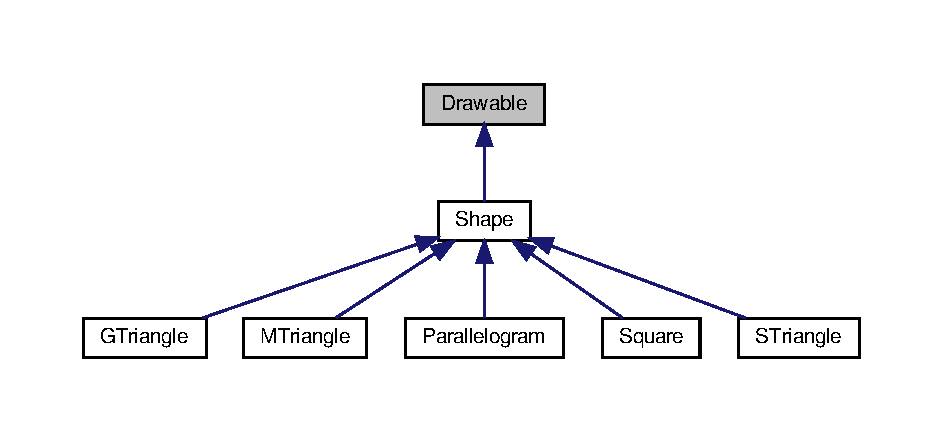
\includegraphics[width=350pt]{classDrawable__inherit__graph}
\end{center}
\end{figure}
\subsection*{Public Member Functions}
\begin{DoxyCompactItemize}
\item 
\mbox{\Hypertarget{classDrawable_a313ec095ce0ea2a8c7cac78a6be27be8}\label{classDrawable_a313ec095ce0ea2a8c7cac78a6be27be8}} 
\hyperlink{classDrawable_a313ec095ce0ea2a8c7cac78a6be27be8}{$\sim$\+I_Drawable} ()=default
\begin{DoxyCompactList}\small\item\em Pure virtual function. Draw everything which needs to be Draw. \end{DoxyCompactList}\item
\mbox{\Hypertarget{classDrawable_aa37d7b328240d343134adcfe5e4dcd38}\label{classDrawable_aa37d7b328240d343134adcfe5e4dcd38}} 
virtual void {\bfseries __Draw} ()=0
\item 
\mbox{\Hypertarget{classDrawable_aa45b93aaf493419c15c240702aa9f692}\label{classDrawable_aa45b93aaf493419c15c240702aa9f692}} 
virtual void {\bfseries iDraw} (M\+L\+V\+\_\+\+Color mColor)=0
\end{DoxyCompactItemize}


\subsection{Detailed Description}
\hyperlink{classDrawable}{I_Drawable} is everything to iDraw.

This class manage everything drawing 

The documentation for this class was generated from the following file\+:\begin{DoxyCompactItemize}
\item 
include/drawable/I_Drawable.\+h\end{DoxyCompactItemize}

\hypertarget{classGame}{}\section{C_Game Class Reference}
\label{classGame}\index{C_Game@{C_Game}}


Class of the main \hyperlink{classGame}{C_Game}.




{\ttfamily \#include $<$C_Game.\+hpp$>$}

\subsection*{Public Member Functions}
\begin{DoxyCompactItemize}
\item 
\mbox{\Hypertarget{classGame_a9e9a77d478f0c0bfb9b61fb1a6556e15}\label{classGame_a9e9a77d478f0c0bfb9b61fb1a6556e15}} 
void \hyperlink{classGame_a9e9a77d478f0c0bfb9b61fb1a6556e15}{main\+\_\+loop} ()
\begin{DoxyCompactList}\small\item\em Main loop of the game. \end{DoxyCompactList}\item 
\mbox{\Hypertarget{classGame_ae3d112ca6e0e55150d2fdbc704474530}\label{classGame_ae3d112ca6e0e55150d2fdbc704474530}} 
\hyperlink{classGame_ae3d112ca6e0e55150d2fdbc704474530}{$\sim$\+C_Game} ()
\begin{DoxyCompactList}\small\item\em Destructor of the game. \end{DoxyCompactList}\item 
\hyperlink{classGame_a2b0cb8af7b823a6d595eef9c9641f806}{C_Game} (int w, int h)
\begin{DoxyCompactList}\small\item\em Constructor of the game, initialize a game with an sizing. \end{DoxyCompactList}\item 
void \hyperlink{classGame_aab43fea0e202c203d998ae575d3f6eeb}{add\+\_\+shape} (std\+::shared\+\_\+ptr$<$ \hyperlink{classShape}{A_Shape} $>$ s)
\begin{DoxyCompactList}\small\item\em Add a shape in the game. \end{DoxyCompactList}\item 
\mbox{\Hypertarget{classGame_a8ba8d7bcda356ed584dc445184320ff7}\label{classGame_a8ba8d7bcda356ed584dc445184320ff7}} 
void \hyperlink{classGame_a8ba8d7bcda356ed584dc445184320ff7}{Clear} ()
\begin{DoxyCompactList}\small\item\em Clear the game / the board and the mObjective. \end{DoxyCompactList}\item
void \hyperlink{classGame_a54ea3746d3738423197219af2d508188}{stick} (const std\+::shared\+\_\+ptr$<$ \hyperlink{classShape}{A_Shape} $>$ \&shape)
\begin{DoxyCompactList}\small\item\em Stick the shape to nearest mObjective mPoints. \end{DoxyCompactList}\item
void \hyperlink{classGame_af8d3ef359625e4179d54f5dd956a0df5}{set\+\_\+\+C_Objective} (const std\+::vector$<$ std\+::shared\+\_\+ptr$<$ \hyperlink{classShape}{A_Shape} $>$$>$ \&vec\+\_\+mObjective)
\begin{DoxyCompactList}\small\item\em Set the mObjective of the game. \end{DoxyCompactList}\item
M\+L\+V\+\_\+\+Color \hyperlink{classGame_ac5de4b11ae90a7ea9182621039fa511c}{get\+\_\+\+C_Objective\+\_\+\+Color} ()
\begin{DoxyCompactList}\small\item\em Get the mColor of the mObjective of the game. \end{DoxyCompactList}\end{DoxyCompactItemize}


\subsection{Detailed Description}
Class of the main \hyperlink{classGame}{C_Game}.

This class manage everything about the main game 

\subsection{Constructor \& Destructor Documentation}
\mbox{\Hypertarget{classGame_a2b0cb8af7b823a6d595eef9c9641f806}\label{classGame_a2b0cb8af7b823a6d595eef9c9641f806}} 
\index{C_Game@{C_Game}!C_Game@{C_Game}}
\index{C_Game@{C_Game}!C_Game@{C_Game}}
\subsubsection{\texorpdfstring{C_Game()}{C_Game()}}
{\footnotesize\ttfamily C_Game\+::\+C_Game (\begin{DoxyParamCaption}\item[{int}]{w,  }\item[{int}]{h }\end{DoxyParamCaption})}



Constructor of the game, initialize a game with an sizing. 


\begin{DoxyParams}{Parameters}
{\em w} & \+: Width of the window \\
\hline
{\em h} & \+: Height of the window \\
\hline
\end{DoxyParams}


\subsection{Member Function Documentation}
\mbox{\Hypertarget{classGame_aab43fea0e202c203d998ae575d3f6eeb}\label{classGame_aab43fea0e202c203d998ae575d3f6eeb}} 
\index{C_Game@{C_Game}!add\+\_\+shape@{add\+\_\+shape}}
\index{add\+\_\+shape@{add\+\_\+shape}!C_Game@{C_Game}}
\subsubsection{\texorpdfstring{add\+\_\+shape()}{add\_shape()}}
{\footnotesize\ttfamily void C_Game\+::add\+\_\+shape (\begin{DoxyParamCaption}\item[{std\+::shared\+\_\+ptr$<$ \hyperlink{classShape}{A_Shape} $>$}]{s }\end{DoxyParamCaption})}



Add a shape in the game. 


\begin{DoxyParams}{Parameters}
{\em s} & \+: \hyperlink{classShape}{A_Shape} to add \\
\hline
\end{DoxyParams}
\mbox{\Hypertarget{classGame_ac5de4b11ae90a7ea9182621039fa511c}\label{classGame_ac5de4b11ae90a7ea9182621039fa511c}} 
\index{C_Game@{C_Game}!get\+\_\+\+C_Objective\+\_\+\+Color@{get\+\_\+\+C_Objective\+\_\+\+Color}}
\index{get\+\_\+\+C_Objective\+\_\+\+Color@{get\+\_\+\+C_Objective\+\_\+\+Color}!C_Game@{C_Game}}
\subsubsection{\texorpdfstring{get\+\_\+\+C_Objective\+\_\+\+Color()}{get\_Objective\_Color()}}
{\footnotesize\ttfamily M\+L\+V\+\_\+\+Color C_Game\+::get\+\_\+\+C_Objective\+\_\+\+Color (\begin{DoxyParamCaption}{ }\end{DoxyParamCaption})}



Get the mColor of the mObjective of the game.

\begin{DoxyReturn}{Returns}
Return the mColor of the mObjective of the game
\end{DoxyReturn}
\mbox{\Hypertarget{classGame_af8d3ef359625e4179d54f5dd956a0df5}\label{classGame_af8d3ef359625e4179d54f5dd956a0df5}} 
\index{C_Game@{C_Game}!set\+\_\+\+C_Objective@{set\+\_\+\+C_Objective}}
\index{set\+\_\+\+C_Objective@{set\+\_\+\+C_Objective}!C_Game@{C_Game}}
\subsubsection{\texorpdfstring{set\+\_\+\+C_Objective()}{set\_Objective()}}
{\footnotesize\ttfamily void C_Game\+::set\+\_\+\+C_Objective (\begin{DoxyParamCaption}\item[{const std\+::vector$<$ std\+::shared\+\_\+ptr$<$ \hyperlink{classShape}{A_Shape} $>$$>$ \&}]{vec\+\_\+mObjective }\end{DoxyParamCaption})}



Set the mObjective of the game.


\begin{DoxyParams}{Parameters}
{\em vec\+\_\+mObjective} & \+: Vector of \hyperlink{classObjective}{C_Objective} for new game; \\
\hline
\end{DoxyParams}
\mbox{\Hypertarget{classGame_a54ea3746d3738423197219af2d508188}\label{classGame_a54ea3746d3738423197219af2d508188}} 
\index{C_Game@{C_Game}!stick@{stick}}
\index{stick@{stick}!C_Game@{C_Game}}
\subsubsection{\texorpdfstring{stick()}{stick()}}
{\footnotesize\ttfamily void C_Game\+::Stick (\begin{DoxyParamCaption}\item[{const std\+::shared\+\_\+ptr$<$ \hyperlink{classShape}{A_Shape} $>$ \&}]{shape }\end{DoxyParamCaption})}



__Stick the shape to nearest mObjective mPoints.


\begin{DoxyParams}{Parameters}
{\em shape} & \+: Last shape rotated or moved \\
\hline
\end{DoxyParams}


The documentation for this class was generated from the following files\+:\begin{DoxyCompactItemize}
\item 
include/game/\hyperlink{Game_8hpp}{C_Game.\+hpp}\item
src/game/C_Game.\+cpp\end{DoxyCompactItemize}

\hypertarget{classGTriangle}{}\section{G\+Triangle Class Reference}
\label{classGTriangle}\index{G\+Triangle@{G\+Triangle}}


Class of the greatest triangle.  




{\ttfamily \#include $<$G\+Triangle.\+hpp$>$}



Inheritance diagram for G\+Triangle\+:\nopagebreak
\begin{figure}[H]
\begin{center}
\leavevmode
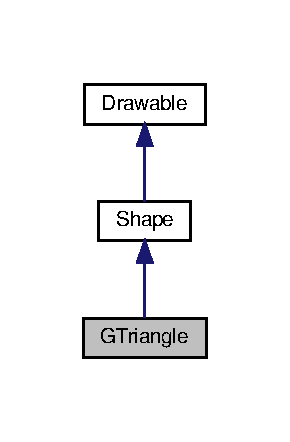
\includegraphics[width=139pt]{classGTriangle__inherit__graph}
\end{center}
\end{figure}


Collaboration diagram for G\+Triangle\+:\nopagebreak
\begin{figure}[H]
\begin{center}
\leavevmode
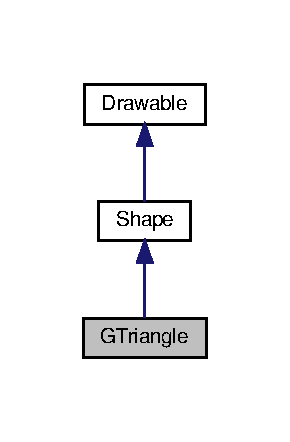
\includegraphics[width=139pt]{classGTriangle__coll__graph}
\end{center}
\end{figure}
\subsection*{Public Member Functions}
\begin{DoxyCompactItemize}
\item 
\mbox{\Hypertarget{classGTriangle_a05bcaee071e6dc6591220869234b05ee}\label{classGTriangle_a05bcaee071e6dc6591220869234b05ee}} 
\hyperlink{classGTriangle_a05bcaee071e6dc6591220869234b05ee}{$\sim$\+G\+Triangle} () override
\begin{DoxyCompactList}\small\item\em Destructor of \hyperlink{classGTriangle}{G\+Triangle}. \end{DoxyCompactList}\item 
\hyperlink{classGTriangle_ad4e9c12fdff32b737ca9e67d64c339bc}{G\+Triangle} (M\+L\+V\+\_\+\+Color color=M\+L\+V\+\_\+\+C\+O\+L\+O\+R\+\_\+\+R\+ED)
\begin{DoxyCompactList}\small\item\em Constructor by default of \hyperlink{classGTriangle}{G\+Triangle}, make a triangle as default. \end{DoxyCompactList}\item 
\hyperlink{classGTriangle_a1b5220a52053342a4aa85499e328b9ea}{G\+Triangle} (const std\+::vector$<$ \hyperlink{classSTriangle}{S\+Triangle} $>$ \&triangle, M\+L\+V\+\_\+\+Color color=M\+L\+V\+\_\+\+C\+O\+L\+O\+R\+\_\+\+R\+ED)
\begin{DoxyCompactList}\small\item\em Constructor of \hyperlink{classGTriangle}{G\+Triangle}, requires a vector of triangles. \end{DoxyCompactList}\item 
\hyperlink{classGTriangle_a1af75c4d0dc8f03e6e4b1b66f0e463ff}{G\+Triangle} (const \hyperlink{classPoint}{Point}$<$ double $>$ \&origin, double angular=0.\+0, M\+L\+V\+\_\+\+Color color=M\+L\+V\+\_\+\+C\+O\+L\+O\+R\+\_\+\+R\+ED)
\begin{DoxyCompactList}\small\item\em Constructor of \hyperlink{classGTriangle}{G\+Triangle}, calls the deleguate Default Constructor. \end{DoxyCompactList}\item 
void \hyperlink{classGTriangle_a6675f3448fca16c1afec576145a9b139}{move} (const \hyperlink{classPoint}{Point}$<$ double $>$ \&translation) override
\begin{DoxyCompactList}\small\item\em Move the \hyperlink{classGTriangle}{G\+Triangle} by point translation. \end{DoxyCompactList}\item 
void \hyperlink{classGTriangle_ae3ed75bbad4ba7fed68bc06c5834cfbe}{rotate} (double angular) override
\begin{DoxyCompactList}\small\item\em Rotate the \hyperlink{classGTriangle}{G\+Triangle} with specified angular. \end{DoxyCompactList}\item 
\mbox{\Hypertarget{classGTriangle_ab223d049ce2518095201b99c8940e724}\label{classGTriangle_ab223d049ce2518095201b99c8940e724}} 
void \hyperlink{classGTriangle_ab223d049ce2518095201b99c8940e724}{flip} () override
\begin{DoxyCompactList}\small\item\em Flip the figure as symmetry. \end{DoxyCompactList}\item 
\mbox{\Hypertarget{classGTriangle_adb7a211b65860ce4dfcc13275cd5052d}\label{classGTriangle_adb7a211b65860ce4dfcc13275cd5052d}} 
void \hyperlink{classGTriangle_adb7a211b65860ce4dfcc13275cd5052d}{draw} () override
\begin{DoxyCompactList}\small\item\em Draw this shape on I\+HM. \end{DoxyCompactList}\item 
bool \hyperlink{classGTriangle_abb6f7243155483cc6de301931e87475a}{is\+\_\+in\+\_\+shape} (const \hyperlink{classPoint}{Point}$<$ double $>$ \&click) override
\begin{DoxyCompactList}\small\item\em Check if a point is in this shape. \end{DoxyCompactList}\item 
std\+::vector$<$ \hyperlink{classPoint}{Point}$<$ double $>$ $>$ \hyperlink{classGTriangle_add4581d1b52836142de5817de4d52d17}{get\+\_\+\+Points} () override
\begin{DoxyCompactList}\small\item\em Get points of this shape. \end{DoxyCompactList}\item 
bool \hyperlink{classGTriangle_adb9dae329128600209c54cc4587480ee}{set\+\_\+\+Points} (const \hyperlink{classPoint}{Point}$<$ double $>$ \&ref, const \hyperlink{classPoint}{Point}$<$ double $>$ \&changed) override
\begin{DoxyCompactList}\small\item\em Pure virtual function. Get all points of this shape. \end{DoxyCompactList}\item 
std\+::string \hyperlink{classGTriangle_a8381aeea39fac0d52ad9e0d45b791b3b}{to\+String} () override
\begin{DoxyCompactList}\small\item\em Convert all data of \hyperlink{classGTriangle}{G\+Triangle} in a string. \end{DoxyCompactList}\end{DoxyCompactItemize}
\subsection*{Additional Inherited Members}


\subsection{Detailed Description}
Class of the greatest triangle. 

This class manage everything about the greatest triangle 

\subsection{Constructor \& Destructor Documentation}
\mbox{\Hypertarget{classGTriangle_ad4e9c12fdff32b737ca9e67d64c339bc}\label{classGTriangle_ad4e9c12fdff32b737ca9e67d64c339bc}} 
\index{G\+Triangle@{G\+Triangle}!G\+Triangle@{G\+Triangle}}
\index{G\+Triangle@{G\+Triangle}!G\+Triangle@{G\+Triangle}}
\subsubsection{\texorpdfstring{G\+Triangle()}{GTriangle()}\hspace{0.1cm}{\footnotesize\ttfamily [1/3]}}
{\footnotesize\ttfamily G\+Triangle\+::\+G\+Triangle (\begin{DoxyParamCaption}\item[{M\+L\+V\+\_\+\+Color}]{color = {\ttfamily MLV\+\_\+COLOR\+\_\+RED} }\end{DoxyParamCaption})\hspace{0.3cm}{\ttfamily [explicit]}}



Constructor by default of \hyperlink{classGTriangle}{G\+Triangle}, make a triangle as default. 


\begin{DoxyParams}{Parameters}
{\em color} & \+: Optional parameter, color of this shape \\
\hline
\end{DoxyParams}
\mbox{\Hypertarget{classGTriangle_a1b5220a52053342a4aa85499e328b9ea}\label{classGTriangle_a1b5220a52053342a4aa85499e328b9ea}} 
\index{G\+Triangle@{G\+Triangle}!G\+Triangle@{G\+Triangle}}
\index{G\+Triangle@{G\+Triangle}!G\+Triangle@{G\+Triangle}}
\subsubsection{\texorpdfstring{G\+Triangle()}{GTriangle()}\hspace{0.1cm}{\footnotesize\ttfamily [2/3]}}
{\footnotesize\ttfamily G\+Triangle\+::\+G\+Triangle (\begin{DoxyParamCaption}\item[{const std\+::vector$<$ \hyperlink{classSTriangle}{S\+Triangle} $>$ \&}]{triangle,  }\item[{M\+L\+V\+\_\+\+Color}]{color = {\ttfamily MLV\+\_\+COLOR\+\_\+RED} }\end{DoxyParamCaption})\hspace{0.3cm}{\ttfamily [explicit]}}



Constructor of \hyperlink{classGTriangle}{G\+Triangle}, requires a vector of triangles. 


\begin{DoxyParams}{Parameters}
{\em triangle} & \+: The \hyperlink{classGTriangle}{G\+Triangle} will created with a vector of \hyperlink{classSTriangle}{S\+Triangle} (4) \\
\hline
{\em color} & \+: Optional parameter, color of this shape \\
\hline
\end{DoxyParams}
\mbox{\Hypertarget{classGTriangle_a1af75c4d0dc8f03e6e4b1b66f0e463ff}\label{classGTriangle_a1af75c4d0dc8f03e6e4b1b66f0e463ff}} 
\index{G\+Triangle@{G\+Triangle}!G\+Triangle@{G\+Triangle}}
\index{G\+Triangle@{G\+Triangle}!G\+Triangle@{G\+Triangle}}
\subsubsection{\texorpdfstring{G\+Triangle()}{GTriangle()}\hspace{0.1cm}{\footnotesize\ttfamily [3/3]}}
{\footnotesize\ttfamily G\+Triangle\+::\+G\+Triangle (\begin{DoxyParamCaption}\item[{const \hyperlink{classPoint}{Point}$<$ double $>$ \&}]{origin,  }\item[{double}]{angular = {\ttfamily 0.0},  }\item[{M\+L\+V\+\_\+\+Color}]{color = {\ttfamily MLV\+\_\+COLOR\+\_\+RED} }\end{DoxyParamCaption})\hspace{0.3cm}{\ttfamily [explicit]}}



Constructor of \hyperlink{classGTriangle}{G\+Triangle}, calls the deleguate Default Constructor. 


\begin{DoxyParams}{Parameters}
{\em origin} & \+: shifts the figure of a translation of the origin \\
\hline
{\em angular} & \+: Optional parameter (angular=0.\+0 as default), rotate the figure with an angular \\
\hline
{\em color} & \+: Optional parameter, color of this shape \\
\hline
\end{DoxyParams}


\subsection{Member Function Documentation}
\mbox{\Hypertarget{classGTriangle_add4581d1b52836142de5817de4d52d17}\label{classGTriangle_add4581d1b52836142de5817de4d52d17}} 
\index{G\+Triangle@{G\+Triangle}!get\+\_\+\+Points@{get\+\_\+\+Points}}
\index{get\+\_\+\+Points@{get\+\_\+\+Points}!G\+Triangle@{G\+Triangle}}
\subsubsection{\texorpdfstring{get\+\_\+\+Points()}{get\_Points()}}
{\footnotesize\ttfamily std\+::vector$<$ \hyperlink{classPoint}{Point}$<$ double $>$ $>$ G\+Triangle\+::get\+\_\+\+Points (\begin{DoxyParamCaption}{ }\end{DoxyParamCaption})\hspace{0.3cm}{\ttfamily [override]}, {\ttfamily [virtual]}}



Get points of this shape. 

\begin{DoxyReturn}{Returns}
Return a vector of points of this shape 
\end{DoxyReturn}


Implements \hyperlink{classShape_add74a5c682840fa4a519242b1ddbd0b5}{Shape}.

\mbox{\Hypertarget{classGTriangle_abb6f7243155483cc6de301931e87475a}\label{classGTriangle_abb6f7243155483cc6de301931e87475a}} 
\index{G\+Triangle@{G\+Triangle}!is\+\_\+in\+\_\+shape@{is\+\_\+in\+\_\+shape}}
\index{is\+\_\+in\+\_\+shape@{is\+\_\+in\+\_\+shape}!G\+Triangle@{G\+Triangle}}
\subsubsection{\texorpdfstring{is\+\_\+in\+\_\+shape()}{is\_in\_shape()}}
{\footnotesize\ttfamily bool G\+Triangle\+::is\+\_\+in\+\_\+shape (\begin{DoxyParamCaption}\item[{const \hyperlink{classPoint}{Point}$<$ double $>$ \&}]{click }\end{DoxyParamCaption})\hspace{0.3cm}{\ttfamily [override]}, {\ttfamily [virtual]}}



Check if a point is in this shape. 


\begin{DoxyParams}{Parameters}
{\em click} & \+: \hyperlink{classPoint}{Point} to check \\
\hline
\end{DoxyParams}
\begin{DoxyReturn}{Returns}
true if click is in this shape, false if not 
\end{DoxyReturn}


Implements \hyperlink{classShape_aa09a621da090e42840b4bec7ffb27620}{Shape}.

\mbox{\Hypertarget{classGTriangle_a6675f3448fca16c1afec576145a9b139}\label{classGTriangle_a6675f3448fca16c1afec576145a9b139}} 
\index{G\+Triangle@{G\+Triangle}!move@{move}}
\index{move@{move}!G\+Triangle@{G\+Triangle}}
\subsubsection{\texorpdfstring{move()}{move()}}
{\footnotesize\ttfamily void G\+Triangle\+::move (\begin{DoxyParamCaption}\item[{const \hyperlink{classPoint}{Point}$<$ double $>$ \&}]{translation }\end{DoxyParamCaption})\hspace{0.3cm}{\ttfamily [override]}, {\ttfamily [virtual]}}



Move the \hyperlink{classGTriangle}{G\+Triangle} by point translation. 


\begin{DoxyParams}{Parameters}
{\em translation} & \+: Every points of this shape will be translate by this parameter \\
\hline
\end{DoxyParams}


Implements \hyperlink{classShape_a1f447acd6219cb10b9b7a40371519c46}{Shape}.

\mbox{\Hypertarget{classGTriangle_ae3ed75bbad4ba7fed68bc06c5834cfbe}\label{classGTriangle_ae3ed75bbad4ba7fed68bc06c5834cfbe}} 
\index{G\+Triangle@{G\+Triangle}!rotate@{rotate}}
\index{rotate@{rotate}!G\+Triangle@{G\+Triangle}}
\subsubsection{\texorpdfstring{rotate()}{rotate()}}
{\footnotesize\ttfamily void G\+Triangle\+::rotate (\begin{DoxyParamCaption}\item[{double}]{angular }\end{DoxyParamCaption})\hspace{0.3cm}{\ttfamily [override]}, {\ttfamily [virtual]}}



Rotate the \hyperlink{classGTriangle}{G\+Triangle} with specified angular. 


\begin{DoxyParams}{Parameters}
{\em angular} & \+: This angular should be between (0, 2\+PI) \\
\hline
\end{DoxyParams}


Implements \hyperlink{classShape_a2dea8616fd40f2d69fd208715921982a}{Shape}.

\mbox{\Hypertarget{classGTriangle_adb9dae329128600209c54cc4587480ee}\label{classGTriangle_adb9dae329128600209c54cc4587480ee}} 
\index{G\+Triangle@{G\+Triangle}!set\+\_\+\+Points@{set\+\_\+\+Points}}
\index{set\+\_\+\+Points@{set\+\_\+\+Points}!G\+Triangle@{G\+Triangle}}
\subsubsection{\texorpdfstring{set\+\_\+\+Points()}{set\_Points()}}
{\footnotesize\ttfamily bool G\+Triangle\+::set\+\_\+\+Points (\begin{DoxyParamCaption}\item[{const \hyperlink{classPoint}{Point}$<$ double $>$ \&}]{ref,  }\item[{const \hyperlink{classPoint}{Point}$<$ double $>$ \&}]{changed }\end{DoxyParamCaption})\hspace{0.3cm}{\ttfamily [override]}, {\ttfamily [virtual]}}



Pure virtual function. Get all points of this shape. 

\begin{DoxyReturn}{Returns}
Return a vector of points of this shape 
\end{DoxyReturn}


Implements \hyperlink{classShape_a6eb0d80cccc44cb72b06c61d9780bc6b}{Shape}.

\mbox{\Hypertarget{classGTriangle_a8381aeea39fac0d52ad9e0d45b791b3b}\label{classGTriangle_a8381aeea39fac0d52ad9e0d45b791b3b}} 
\index{G\+Triangle@{G\+Triangle}!to\+String@{to\+String}}
\index{to\+String@{to\+String}!G\+Triangle@{G\+Triangle}}
\subsubsection{\texorpdfstring{to\+String()}{toString()}}
{\footnotesize\ttfamily std\+::string G\+Triangle\+::to\+String (\begin{DoxyParamCaption}{ }\end{DoxyParamCaption})\hspace{0.3cm}{\ttfamily [override]}, {\ttfamily [virtual]}}



Convert all data of \hyperlink{classGTriangle}{G\+Triangle} in a string. 

\begin{DoxyReturn}{Returns}
Return a string which contains every points of this shape 
\end{DoxyReturn}


Implements \hyperlink{classShape_a98fa87c6dc4c7045fd6897a8f3bc186c}{Shape}.



The documentation for this class was generated from the following files\+:\begin{DoxyCompactItemize}
\item 
include/shape/\hyperlink{GTriangle_8hpp}{G\+Triangle.\+hpp}\item 
src/shape/G\+Triangle.\+cpp\end{DoxyCompactItemize}

\hypertarget{classLoader}{}\section{C_Loader Class Reference}
\label{classLoader}\index{C_Loader@{C_Loader}}


Class of the main \hyperlink{classLoader}{C_Loader}.




{\ttfamily \#include $<$C_Loader.\+hpp$>$}

\subsection*{Static Public Member Functions}
\begin{DoxyCompactItemize}
\item 
static bool \hyperlink{classLoader_a22ccbf4c21a330d16e37b99948d43ddb}{parse\+\_\+file} (const std\+::string \&filename, \hyperlink{classGame}{C_Game} \&game)
\begin{DoxyCompactList}\small\item\em Parse a file to make a board. \end{DoxyCompactList}\end{DoxyCompactItemize}


\subsection{Detailed Description}
Class of the main \hyperlink{classLoader}{C_Loader}.

This class manage everything about the loader 

\subsection{Member Function Documentation}
\mbox{\Hypertarget{classLoader_a22ccbf4c21a330d16e37b99948d43ddb}\label{classLoader_a22ccbf4c21a330d16e37b99948d43ddb}} 
\index{C_Loader@{C_Loader}!parse\+\_\+file@{parse\+\_\+file}}
\index{parse\+\_\+file@{parse\+\_\+file}!C_Loader@{C_Loader}}
\subsubsection{\texorpdfstring{parse\+\_\+file()}{parse\_file()}}
{\footnotesize\ttfamily bool C_Loader\+::parse\+\_\+file (\begin{DoxyParamCaption}\item[{const std\+::string \&}]{filename,  }\item[{\hyperlink{classGame}{C_Game} \&}]{game }\end{DoxyParamCaption})\hspace{0.3cm}{\ttfamily [static]}}



Parse a file to make a board. 


\begin{DoxyParams}{Parameters}
{\em filename} & \+: name of the file, this file should be located in this directory ./\+Tangram/extern/board/ \\
\hline
{\em game} & \+: The current game / board \\
\hline
\end{DoxyParams}
\begin{DoxyReturn}{Returns}
True if the game has been created, false if not 
\end{DoxyReturn}


The documentation for this class was generated from the following files\+:\begin{DoxyCompactItemize}
\item 
include/parser/\hyperlink{Loader_8hpp}{C_Loader.\+hpp}\item
src/parser/C_Loader.\+cpp\end{DoxyCompactItemize}

\hypertarget{classMenu}{}\section{C_Menu Class Reference}
\label{classMenu}\index{C_Menu@{C_Menu}}


\hyperlink{classMenu}{C_Menu} of the game.




{\ttfamily \#include $<$C_Menu.\+hpp$>$}

\subsection*{Public Member Functions}
\begin{DoxyCompactItemize}
\item 
void \hyperlink{classMenu_aaf6a2fb4408f8d5b5bdd7e633da53193}{add\+\_\+button} (const \hyperlink{classButton}{C_Button} \&button)
\begin{DoxyCompactList}\small\item\em Add a button in the \hyperlink{classMenu}{C_Menu}. \end{DoxyCompactList}\item
\mbox{\Hypertarget{classMenu_a02baf39291517cea771a2e1cffed960e}\label{classMenu_a02baf39291517cea771a2e1cffed960e}} 
void \hyperlink{classMenu_a02baf39291517cea771a2e1cffed960e}{main\+\_\+loop} ()
\begin{DoxyCompactList}\small\item\em Main loop of the \hyperlink{classMenu}{C_Menu}. \end{DoxyCompactList}\end{DoxyCompactItemize}


\subsection{Detailed Description}
\hyperlink{classMenu}{C_Menu} of the game.

This class manage everything about Tangram\textquotesingle{}s menu 

\subsection{Member Function Documentation}
\mbox{\Hypertarget{classMenu_aaf6a2fb4408f8d5b5bdd7e633da53193}\label{classMenu_aaf6a2fb4408f8d5b5bdd7e633da53193}} 
\index{C_Menu@{C_Menu}!add\+\_\+button@{add\+\_\+button}}
\index{add\+\_\+button@{add\+\_\+button}!C_Menu@{C_Menu}}
\subsubsection{\texorpdfstring{add\+\_\+button()}{add\_button()}}
{\footnotesize\ttfamily void C_Menu\+::add\+\_\+button (\begin{DoxyParamCaption}\item[{const \hyperlink{classButton}{C_Button} \&}]{button }\end{DoxyParamCaption})}



Add a button in the \hyperlink{classMenu}{C_Menu}.


\begin{DoxyParams}{Parameters}
{\em button} & \+: \hyperlink{classButton}{C_Button} to add \\
\hline
\end{DoxyParams}


The documentation for this class was generated from the following files\+:\begin{DoxyCompactItemize}
\item 
include/drawable/\hyperlink{Menu_8hpp}{C_Menu.\+hpp}\item
src/drawable/C_Menu.\+cpp\end{DoxyCompactItemize}

\hypertarget{classMTriangle}{}\section{M\+Triangle Class Reference}
\label{classMTriangle}\index{M\+Triangle@{M\+Triangle}}


Class of the medium triangle.  




{\ttfamily \#include $<$M\+Triangle.\+hpp$>$}



Inheritance diagram for M\+Triangle\+:
\nopagebreak
\begin{figure}[H]
\begin{center}
\leavevmode
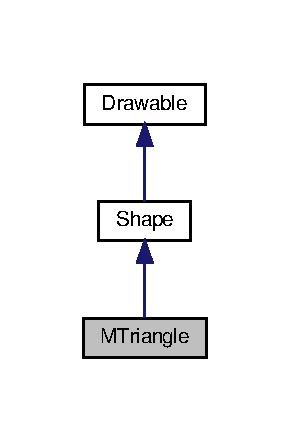
\includegraphics[width=139pt]{classMTriangle__inherit__graph}
\end{center}
\end{figure}


Collaboration diagram for M\+Triangle\+:
\nopagebreak
\begin{figure}[H]
\begin{center}
\leavevmode
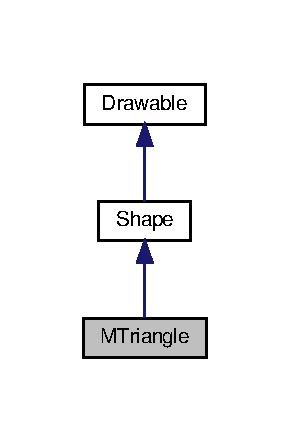
\includegraphics[width=139pt]{classMTriangle__coll__graph}
\end{center}
\end{figure}
\subsection*{Public Member Functions}
\begin{DoxyCompactItemize}
\item 
\mbox{\Hypertarget{classMTriangle_aad494b73728c03ca00e728b0c505a88f}\label{classMTriangle_aad494b73728c03ca00e728b0c505a88f}} 
\hyperlink{classMTriangle_aad494b73728c03ca00e728b0c505a88f}{$\sim$\+M\+Triangle} () override
\begin{DoxyCompactList}\small\item\em Destructor of \hyperlink{classMTriangle}{M\+Triangle}. \end{DoxyCompactList}\item 
\mbox{\Hypertarget{classMTriangle_adca17cfca7632c5967437a7c7e292598}\label{classMTriangle_adca17cfca7632c5967437a7c7e292598}} 
\hyperlink{classMTriangle_adca17cfca7632c5967437a7c7e292598}{M\+Triangle} ()
\begin{DoxyCompactList}\small\item\em Constructor by default of \hyperlink{classMTriangle}{M\+Triangle}, make a \hyperlink{classMTriangle}{M\+Triangle} as default. \end{DoxyCompactList}\item 
\hyperlink{classMTriangle_a428bc13e1f5299369e5c78602aae544b}{M\+Triangle} (const std\+::vector$<$ \hyperlink{classSTriangle}{S\+Triangle} $>$ \&triangle)
\begin{DoxyCompactList}\small\item\em Constructor of \hyperlink{classMTriangle}{M\+Triangle}, requires a vector of S\+Triangles. \end{DoxyCompactList}\item 
\hyperlink{classMTriangle_aaf64b05da66c9196dcddbd0e4791096f}{M\+Triangle} (\hyperlink{classPoint}{Point}$<$ double $>$ origin, double angular=0.\+0)
\begin{DoxyCompactList}\small\item\em Constructor of \hyperlink{classMTriangle}{M\+Triangle}, calls the deleguate Default Constructor. \end{DoxyCompactList}\item 
void \hyperlink{classMTriangle_a1b029feefcf7e3febcdae179557b4c2e}{move} (\hyperlink{classPoint}{Point}$<$ double $>$ translation) override
\begin{DoxyCompactList}\small\item\em Move the \hyperlink{classMTriangle}{M\+Triangle} by point translation. \end{DoxyCompactList}\item 
void \hyperlink{classMTriangle_a4be29553eeddf99c367b1ec220bc102b}{rotate} (double angular) override
\begin{DoxyCompactList}\small\item\em Rotate the \hyperlink{classMTriangle}{M\+Triangle} with specified angular. \end{DoxyCompactList}\item 
\mbox{\Hypertarget{classMTriangle_a6258b96b57c1892098f84a5a5fa0f976}\label{classMTriangle_a6258b96b57c1892098f84a5a5fa0f976}} 
void \hyperlink{classMTriangle_a6258b96b57c1892098f84a5a5fa0f976}{flip} () override
\begin{DoxyCompactList}\small\item\em Flip the figure as symmetry. \end{DoxyCompactList}\item 
\mbox{\Hypertarget{classMTriangle_a7801818e2188f39ba89a2a82df8fa5fe}\label{classMTriangle_a7801818e2188f39ba89a2a82df8fa5fe}} 
void \hyperlink{classMTriangle_a7801818e2188f39ba89a2a82df8fa5fe}{draw} () override
\begin{DoxyCompactList}\small\item\em Draw this shape on I\+HM. \end{DoxyCompactList}\item 
bool \hyperlink{classMTriangle_a8d3d737a903823bf1a631cbb004a799c}{is\+\_\+in\+\_\+shape} (\hyperlink{classPoint}{Point}$<$ double $>$ click) override
\begin{DoxyCompactList}\small\item\em Check if a point is in this shape. \end{DoxyCompactList}\item 
std\+::string \hyperlink{classMTriangle_a7d1fd825592dffa6ac05b3398a8c105a}{to\+String} () override
\begin{DoxyCompactList}\small\item\em Convert all data of \hyperlink{classMTriangle}{M\+Triangle} in a string. \end{DoxyCompactList}\end{DoxyCompactItemize}


\subsection{Detailed Description}
Class of the medium triangle. 

This class manage everything about the medium triangle 

\subsection{Constructor \& Destructor Documentation}
\mbox{\Hypertarget{classMTriangle_a428bc13e1f5299369e5c78602aae544b}\label{classMTriangle_a428bc13e1f5299369e5c78602aae544b}} 
\index{M\+Triangle@{M\+Triangle}!M\+Triangle@{M\+Triangle}}
\index{M\+Triangle@{M\+Triangle}!M\+Triangle@{M\+Triangle}}
\subsubsection{\texorpdfstring{M\+Triangle()}{MTriangle()}\hspace{0.1cm}{\footnotesize\ttfamily [1/2]}}
{\footnotesize\ttfamily M\+Triangle\+::\+M\+Triangle (\begin{DoxyParamCaption}\item[{const std\+::vector$<$ \hyperlink{classSTriangle}{S\+Triangle} $>$ \&}]{triangle }\end{DoxyParamCaption})\hspace{0.3cm}{\ttfamily [explicit]}}



Constructor of \hyperlink{classMTriangle}{M\+Triangle}, requires a vector of S\+Triangles. 


\begin{DoxyParams}{Parameters}
{\em triangle} & \+: The \hyperlink{classMTriangle}{M\+Triangle} will created with a vector of \hyperlink{classSTriangle}{S\+Triangle} (4) \\
\hline
\end{DoxyParams}
\mbox{\Hypertarget{classMTriangle_aaf64b05da66c9196dcddbd0e4791096f}\label{classMTriangle_aaf64b05da66c9196dcddbd0e4791096f}} 
\index{M\+Triangle@{M\+Triangle}!M\+Triangle@{M\+Triangle}}
\index{M\+Triangle@{M\+Triangle}!M\+Triangle@{M\+Triangle}}
\subsubsection{\texorpdfstring{M\+Triangle()}{MTriangle()}\hspace{0.1cm}{\footnotesize\ttfamily [2/2]}}
{\footnotesize\ttfamily M\+Triangle\+::\+M\+Triangle (\begin{DoxyParamCaption}\item[{\hyperlink{classPoint}{Point}$<$ double $>$}]{origin,  }\item[{double}]{angular = {\ttfamily 0.0} }\end{DoxyParamCaption})\hspace{0.3cm}{\ttfamily [explicit]}}



Constructor of \hyperlink{classMTriangle}{M\+Triangle}, calls the deleguate Default Constructor. 


\begin{DoxyParams}{Parameters}
{\em origin} & \+: shifts the figure of a translation of the origin \\
\hline
{\em angular} & \+: Optional parameter (angular=0.\+0 as default), rotate the figure with an angular \\
\hline
\end{DoxyParams}


\subsection{Member Function Documentation}
\mbox{\Hypertarget{classMTriangle_a8d3d737a903823bf1a631cbb004a799c}\label{classMTriangle_a8d3d737a903823bf1a631cbb004a799c}} 
\index{M\+Triangle@{M\+Triangle}!is\+\_\+in\+\_\+shape@{is\+\_\+in\+\_\+shape}}
\index{is\+\_\+in\+\_\+shape@{is\+\_\+in\+\_\+shape}!M\+Triangle@{M\+Triangle}}
\subsubsection{\texorpdfstring{is\+\_\+in\+\_\+shape()}{is\_in\_shape()}}
{\footnotesize\ttfamily bool M\+Triangle\+::is\+\_\+in\+\_\+shape (\begin{DoxyParamCaption}\item[{\hyperlink{classPoint}{Point}$<$ double $>$}]{click }\end{DoxyParamCaption})\hspace{0.3cm}{\ttfamily [override]}, {\ttfamily [virtual]}}



Check if a point is in this shape. 


\begin{DoxyParams}{Parameters}
{\em click} & \+: \hyperlink{classPoint}{Point} to check \\
\hline
\end{DoxyParams}
\begin{DoxyReturn}{Returns}
true if click is in this shape, false if not 
\end{DoxyReturn}


Implements \hyperlink{classShape_abcce23128cd35989468a88a7194152af}{Shape}.

\mbox{\Hypertarget{classMTriangle_a1b029feefcf7e3febcdae179557b4c2e}\label{classMTriangle_a1b029feefcf7e3febcdae179557b4c2e}} 
\index{M\+Triangle@{M\+Triangle}!move@{move}}
\index{move@{move}!M\+Triangle@{M\+Triangle}}
\subsubsection{\texorpdfstring{move()}{move()}}
{\footnotesize\ttfamily void M\+Triangle\+::move (\begin{DoxyParamCaption}\item[{\hyperlink{classPoint}{Point}$<$ double $>$}]{translation }\end{DoxyParamCaption})\hspace{0.3cm}{\ttfamily [override]}, {\ttfamily [virtual]}}



Move the \hyperlink{classMTriangle}{M\+Triangle} by point translation. 


\begin{DoxyParams}{Parameters}
{\em translation} & \+: Every points of this shape will be translate by this parameter \\
\hline
\end{DoxyParams}


Implements \hyperlink{classShape_a52649731b2cb7b67315882d5e005f7e8}{Shape}.

\mbox{\Hypertarget{classMTriangle_a4be29553eeddf99c367b1ec220bc102b}\label{classMTriangle_a4be29553eeddf99c367b1ec220bc102b}} 
\index{M\+Triangle@{M\+Triangle}!rotate@{rotate}}
\index{rotate@{rotate}!M\+Triangle@{M\+Triangle}}
\subsubsection{\texorpdfstring{rotate()}{rotate()}}
{\footnotesize\ttfamily void M\+Triangle\+::rotate (\begin{DoxyParamCaption}\item[{double}]{angular }\end{DoxyParamCaption})\hspace{0.3cm}{\ttfamily [override]}, {\ttfamily [virtual]}}



Rotate the \hyperlink{classMTriangle}{M\+Triangle} with specified angular. 


\begin{DoxyParams}{Parameters}
{\em angular} & \+: This angular should be between (0, 2\+PI) \\
\hline
\end{DoxyParams}


Implements \hyperlink{classShape_a2dea8616fd40f2d69fd208715921982a}{Shape}.

\mbox{\Hypertarget{classMTriangle_a7d1fd825592dffa6ac05b3398a8c105a}\label{classMTriangle_a7d1fd825592dffa6ac05b3398a8c105a}} 
\index{M\+Triangle@{M\+Triangle}!to\+String@{to\+String}}
\index{to\+String@{to\+String}!M\+Triangle@{M\+Triangle}}
\subsubsection{\texorpdfstring{to\+String()}{toString()}}
{\footnotesize\ttfamily std\+::string M\+Triangle\+::to\+String (\begin{DoxyParamCaption}{ }\end{DoxyParamCaption})\hspace{0.3cm}{\ttfamily [override]}, {\ttfamily [virtual]}}



Convert all data of \hyperlink{classMTriangle}{M\+Triangle} in a string. 

\begin{DoxyReturn}{Returns}
Return a string which contains every points of this shape 
\end{DoxyReturn}


Implements \hyperlink{classShape_a98fa87c6dc4c7045fd6897a8f3bc186c}{Shape}.



The documentation for this class was generated from the following files\+:\begin{DoxyCompactItemize}
\item 
include/shape/\hyperlink{MTriangle_8hpp}{M\+Triangle.\+hpp}\item 
src/shape/M\+Triangle.\+cpp\end{DoxyCompactItemize}

\hypertarget{classObjective}{}\section{C_Objective Class Reference}
\label{classObjective}\index{C_Objective@{C_Objective}}


Class of the board \hyperlink{classObjective}{C_Objective}.




{\ttfamily \#include $<$C_Objective.\+hpp$>$}

\subsection*{Public Member Functions}
\begin{DoxyCompactItemize}
\item 
\hyperlink{classObjective_ae515d38979a806a95f9476f4437311ab}{C_Objective} (M\+L\+V\+\_\+\+Color mColor=M\+L\+V\+\_\+\+C\+O\+L\+O\+R\+\_\+\+G\+R\+A\+Y70)
\begin{DoxyCompactList}\small\item\em Constructor of an mObjective, default constructor. \end{DoxyCompactList}\item
\hyperlink{classObjective_a7b72b9e9f9174ec9ee98e3a0a28773f2}{C_Objective} (const std\+::vector$<$ std\+::shared\+\_\+ptr$<$ \hyperlink{classShape}{A_Shape} $>$$>$ \&mObjective, M\+L\+V\+\_\+\+Color mColor=M\+L\+V\+\_\+\+C\+O\+L\+O\+R\+\_\+\+G\+R\+A\+Y70)
\begin{DoxyCompactList}\small\item\em Constructor of an mObjective. \end{DoxyCompactList}\item
std\+::vector$<$ std\+::shared\+\_\+ptr$<$ \hyperlink{classShape}{A_Shape} $>$ $>$ \hyperlink{classObjective_a9d379ffa32a62fbb5e5df62a88201baf}{get\+\_\+\+C_Objective} ()
\begin{DoxyCompactList}\small\item\em Get all shape of the mObjective. \end{DoxyCompactList}\item
M\+L\+V\+\_\+\+Color \hyperlink{classObjective_ae20161454cf0dd248b8e17989044eb13}{get\+\_\+\+Color} ()
\begin{DoxyCompactList}\small\item\em Get the mColor of an \hyperlink{classObjective}{C_Objective}. \end{DoxyCompactList}\end{DoxyCompactItemize}
\subsection*{Static Public Member Functions}
\begin{DoxyCompactItemize}
\item 
static bool \hyperlink{classObjective_aba5fe938ebccb3825d6b03cd789d6d61}{board\+Completed} (const std\+::vector$<$ std\+::shared\+\_\+ptr$<$ \hyperlink{classShape}{A_Shape} $>$$>$ \&mObjective, const std\+::vector$<$ std\+::shared\+\_\+ptr$<$ \hyperlink{classShape}{A_Shape} $>$$>$ \&game)
\begin{DoxyCompactList}\small\item\em Check if the board is mCompleted. \end{DoxyCompactList}\item
static void \hyperlink{classObjective_adecebbf5e11f3e778b1b7f48735a0765}{set\+\_\+\+C_Objective} (std\+::shared\+\_\+ptr$<$ \hyperlink{classObjective}{C_Objective} $>$ mObjective, const std\+::vector$<$ std\+::shared\+\_\+ptr$<$ \hyperlink{classShape}{A_Shape} $>$$>$ \&vec\+\_\+mObjective)
\begin{DoxyCompactList}\small\item\em Set an \hyperlink{classObjective}{C_Objective} for a new game. \end{DoxyCompactList}\end{DoxyCompactItemize}


\subsection{Detailed Description}
Class of the board \hyperlink{classObjective}{C_Objective}.

This class manage everything about the mObjective

\subsection{Constructor \& Destructor Documentation}
\mbox{\Hypertarget{classObjective_ae515d38979a806a95f9476f4437311ab}\label{classObjective_ae515d38979a806a95f9476f4437311ab}} 
\index{C_Objective@{C_Objective}!C_Objective@{C_Objective}}
\index{C_Objective@{C_Objective}!C_Objective@{C_Objective}}
\subsubsection{\texorpdfstring{C_Objective()}{C_Objective()}\hspace{0.1cm}{\footnotesize\ttfamily [1/2]}}
{\footnotesize\ttfamily C_Objective\+::\+C_Objective (\begin{DoxyParamCaption}\item[{M\+L\+V\+\_\+\+Color}]{mColor = {\ttfamily MLV\+\_\+COLOR\+\_\+GRAY70} }\end{DoxyParamCaption})\hspace{0.3cm}{\ttfamily [explicit]}}



Constructor of an mObjective, default constructor.


\begin{DoxyParams}{Parameters}
{\em mColor} & \+: mColor of the mObjective shape \\
\hline
\end{DoxyParams}
\mbox{\Hypertarget{classObjective_a7b72b9e9f9174ec9ee98e3a0a28773f2}\label{classObjective_a7b72b9e9f9174ec9ee98e3a0a28773f2}} 
\index{C_Objective@{C_Objective}!C_Objective@{C_Objective}}
\index{C_Objective@{C_Objective}!C_Objective@{C_Objective}}
\subsubsection{\texorpdfstring{C_Objective()}{C_Objective()}\hspace{0.1cm}{\footnotesize\ttfamily [2/2]}}
{\footnotesize\ttfamily C_Objective\+::\+C_Objective (\begin{DoxyParamCaption}\item[{const std\+::vector$<$ std\+::shared\+\_\+ptr$<$ \hyperlink{classShape}{A_Shape} $>$$>$ \&}]{mObjective,  }\item[{M\+L\+V\+\_\+\+Color}]{mColor = {\ttfamily MLV\+\_\+COLOR\+\_\+GRAY70} }\end{DoxyParamCaption})\hspace{0.3cm}{\ttfamily [explicit]}}



Constructor of an mObjective.


\begin{DoxyParams}{Parameters}
{\em mObjective} & \+: \hyperlink{classObjective}{C_Objective} requires a vector of \hyperlink{classShape}{A_Shape} \\
\hline
{\em mColor} & \+: mColor of the mObjective shape \\
\hline
\end{DoxyParams}


\subsection{Member Function Documentation}
\mbox{\Hypertarget{classObjective_aba5fe938ebccb3825d6b03cd789d6d61}\label{classObjective_aba5fe938ebccb3825d6b03cd789d6d61}} 
\index{C_Objective@{C_Objective}!board\+Completed@{board\+Completed}}
\index{board\+Completed@{board\+Completed}!C_Objective@{C_Objective}}
\subsubsection{\texorpdfstring{board\+Completed()}{BoardCompleted()}}
{\footnotesize\ttfamily bool C_Objective\+::board\+Completed (\begin{DoxyParamCaption}\item[{const std\+::vector$<$ std\+::shared\+\_\+ptr$<$ \hyperlink{classShape}{A_Shape} $>$$>$ \&}]{mObjective,  }\item[{const std\+::vector$<$ std\+::shared\+\_\+ptr$<$ \hyperlink{classShape}{A_Shape} $>$$>$ \&}]{game }\end{DoxyParamCaption})\hspace{0.3cm}{\ttfamily [static]}}



Check if the board is mCompleted.


\begin{DoxyParams}{Parameters}
{\em mObjective} & \+: Vector of mObjective\textquotesingle{}s shape \\
\hline
{\em game} & \+: Vector of current game\textquotesingle{}s shape \\
\hline
\end{DoxyParams}
\begin{DoxyReturn}{Returns}
True if the board is mCompleted, false if not
\end{DoxyReturn}
\mbox{\Hypertarget{classObjective_ae20161454cf0dd248b8e17989044eb13}\label{classObjective_ae20161454cf0dd248b8e17989044eb13}} 
\index{C_Objective@{C_Objective}!get\+\_\+\+Color@{get\+\_\+\+Color}}
\index{get\+\_\+\+Color@{get\+\_\+\+Color}!C_Objective@{C_Objective}}
\subsubsection{\texorpdfstring{get\+\_\+\+Color()}{get\_Color()}}
{\footnotesize\ttfamily M\+L\+V\+\_\+\+Color C_Objective\+::get\+\_\+\+Color (\begin{DoxyParamCaption}{ }\end{DoxyParamCaption})}



Get the mColor of an \hyperlink{classObjective}{C_Objective}.

\begin{DoxyReturn}{Returns}
Return the mColor of an \hyperlink{classObjective}{C_Objective}
\end{DoxyReturn}
\mbox{\Hypertarget{classObjective_a9d379ffa32a62fbb5e5df62a88201baf}\label{classObjective_a9d379ffa32a62fbb5e5df62a88201baf}} 
\index{C_Objective@{C_Objective}!get\+\_\+\+C_Objective@{get\+\_\+\+C_Objective}}
\index{get\+\_\+\+C_Objective@{get\+\_\+\+C_Objective}!C_Objective@{C_Objective}}
\subsubsection{\texorpdfstring{get\+\_\+\+C_Objective()}{get\_Objective()}}
{\footnotesize\ttfamily std\+::vector$<$ std\+::shared\+\_\+ptr$<$ \hyperlink{classShape}{A_Shape} $>$ $>$ C_Objective\+::get\+\_\+\+C_Objective (\begin{DoxyParamCaption}{ }\end{DoxyParamCaption})}



Get all shape of the mObjective.

\begin{DoxyReturn}{Returns}
Return a vector of shape of the mObjective
\end{DoxyReturn}
\mbox{\Hypertarget{classObjective_adecebbf5e11f3e778b1b7f48735a0765}\label{classObjective_adecebbf5e11f3e778b1b7f48735a0765}} 
\index{C_Objective@{C_Objective}!set\+\_\+\+C_Objective@{set\+\_\+\+C_Objective}}
\index{set\+\_\+\+C_Objective@{set\+\_\+\+C_Objective}!C_Objective@{C_Objective}}
\subsubsection{\texorpdfstring{set\+\_\+\+C_Objective()}{set\_Objective()}}
{\footnotesize\ttfamily void C_Objective\+::set\+\_\+\+C_Objective (\begin{DoxyParamCaption}\item[{std\+::shared\+\_\+ptr$<$ \hyperlink{classObjective}{C_Objective} $>$}]{mObjective,  }\item[{const std\+::vector$<$ std\+::shared\+\_\+ptr$<$ \hyperlink{classShape}{A_Shape} $>$$>$ \&}]{vec\+\_\+mObjective }\end{DoxyParamCaption})\hspace{0.3cm}{\ttfamily [static]}}



Set an \hyperlink{classObjective}{C_Objective} for a new game.


\begin{DoxyParams}{Parameters}
{\em mObjective} & \+: \hyperlink{classObjective}{C_Objective} to mUpdate \\
\hline
{\em vec\+\_\+mObjective} & \+:Vector of new \hyperlink{classShape}{A_Shape} for the new \hyperlink{classObjective}{C_Objective} \\
\hline
\end{DoxyParams}


The documentation for this class was generated from the following files\+:\begin{DoxyCompactItemize}
\item 
include/game/\hyperlink{Objective_8hpp}{C_Objective.\+hpp}\item
src/game/C_Objective.\+cpp\end{DoxyCompactItemize}

\hypertarget{classParallelogram}{}\section{C_Parallelogram Class Reference}
\label{classParallelogram}\index{C_Parallelogram@{C_Parallelogram}}


Class of the parallelogram.  




{\ttfamily \#include $<$C_Parallelogram.\+hpp$>$}



Inheritance diagram for C_Parallelogram\+:\nopagebreak
\begin{figure}[H]
\begin{center}
\leavevmode
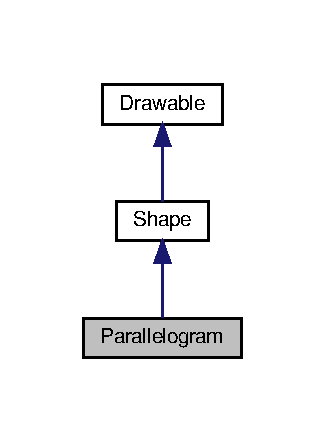
\includegraphics[width=156pt]{classParallelogram__inherit__graph}
\end{center}
\end{figure}


Collaboration diagram for C_Parallelogram\+:\nopagebreak
\begin{figure}[H]
\begin{center}
\leavevmode
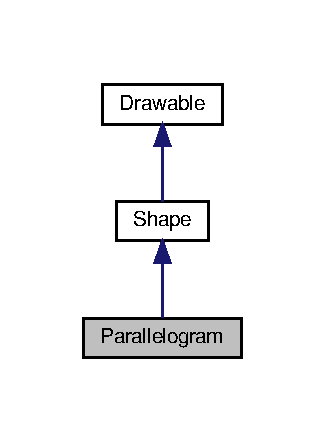
\includegraphics[width=156pt]{classParallelogram__coll__graph}
\end{center}
\end{figure}
\subsection*{Public Member Functions}
\begin{DoxyCompactItemize}
\item 
\mbox{\Hypertarget{classParallelogram_ae3c14e58b92406f4679234817313a26c}\label{classParallelogram_ae3c14e58b92406f4679234817313a26c}} 
\hyperlink{classParallelogram_ae3c14e58b92406f4679234817313a26c}{$\sim$\+C_Parallelogram} () override
\begin{DoxyCompactList}\small\item\em Destructor of \hyperlink{classParallelogram}{C_Parallelogram}. \end{DoxyCompactList}\item
\hyperlink{classParallelogram_a2200aa50be9b13ccb40a371a3d2b119b}{C_Parallelogram} (M\+L\+V\+\_\+\+Color mColor=M\+L\+V\+\_\+\+C\+O\+L\+O\+R\+\_\+\+B\+L\+UE)
\begin{DoxyCompactList}\small\item\em Constructor by default of \hyperlink{classParallelogram}{C_Parallelogram}, make a \hyperlink{classParallelogram}{C_Parallelogram} as default. \end{DoxyCompactList}\item
\hyperlink{classParallelogram_ac60d6fc9e306b202e9c679d170d6d063}{C_Parallelogram} (const std\+::vector$<$ \hyperlink{classSTriangle}{S\+Triangle} $>$ \&mTriangles, M\+L\+V\+\_\+\+Color mColor=M\+L\+V\+\_\+\+C\+O\+L\+O\+R\+\_\+\+B\+L\+UE)
\begin{DoxyCompactList}\small\item\em Constructor of \hyperlink{classParallelogram}{C_Parallelogram}, requires a vector of S\+Triangles. \end{DoxyCompactList}\item
\hyperlink{classParallelogram_aeed0c83e942a4869b79d4baab00c2874}{C_Parallelogram} (const \hyperlink{classPoint}{T_Point}$<$ double $>$ \&origin, double angular=0.\+0, M\+L\+V\+\_\+\+Color mColor=M\+L\+V\+\_\+\+C\+O\+L\+O\+R\+\_\+\+B\+L\+UE)
\begin{DoxyCompactList}\small\item\em Constructor of \hyperlink{classParallelogram}{C_Parallelogram}, calls the deleguate Default Constructor. \end{DoxyCompactList}\item
void \hyperlink{classParallelogram_ae8d51f9b629160df31c8a12c28da279e}{move} (const \hyperlink{classPoint}{T_Point}$<$ double $>$ \&translation) override
\begin{DoxyCompactList}\small\item\em Move the \hyperlink{classParallelogram}{C_Parallelogram} by point translation. \end{DoxyCompactList}\item
void \hyperlink{classParallelogram_ac498f6a15dea236ecc49bece023d17b0}{rotate} (double angular) override
\begin{DoxyCompactList}\small\item\em Rotate the \hyperlink{classParallelogram}{C_Parallelogram} with specified angular. \end{DoxyCompactList}\item
\mbox{\Hypertarget{classParallelogram_a51f002e90b7bf6c5d875cc094c22f7c1}\label{classParallelogram_a51f002e90b7bf6c5d875cc094c22f7c1}} 
void \hyperlink{classParallelogram_a51f002e90b7bf6c5d875cc094c22f7c1}{aFlip} () override
\begin{DoxyCompactList}\small\item\em Flip the figure as symmetry. \end{DoxyCompactList}\item 
\mbox{\Hypertarget{classParallelogram_a73e3657bf024787b57ccdd8035a6fdef}\label{classParallelogram_a73e3657bf024787b57ccdd8035a6fdef}} 
void \hyperlink{classParallelogram_a73e3657bf024787b57ccdd8035a6fdef}{iDraw} () override
\begin{DoxyCompactList}\small\item\em Draw this shape on I\+HM. \end{DoxyCompactList}\item 
\mbox{\Hypertarget{classParallelogram_a4c819c66cd206e71a86e863e266ff356}\label{classParallelogram_a4c819c66cd206e71a86e863e266ff356}} 
void {\bfseries iDraw} (M\+L\+V\+\_\+\+Color mColor) override
\item 
bool \hyperlink{classParallelogram_a585b14ca0f65ed3a5007e8c1df3c6bc4}{is\+\_\+in\+\_\+shape} (const \hyperlink{classPoint}{T_Point}$<$ double $>$ \&click) override
\begin{DoxyCompactList}\small\item\em Check if a point is in this shape. \end{DoxyCompactList}\item 
std\+::vector$<$ \hyperlink{classPoint}{T_Point}$<$ double $>$ $>$ \hyperlink{classParallelogram_a17c9986712806a8b07d90e444e0a543d}{get\+\_\+\+Points} () override
\begin{DoxyCompactList}\small\item\em Get mPoints of this shape. \end{DoxyCompactList}\item
bool \hyperlink{classParallelogram_ab74583703a60e4b798d7048aa684f44e}{set\+\_\+\+Points} (const \hyperlink{classPoint}{T_Point}$<$ double $>$ \&ref, const \hyperlink{classPoint}{T_Point}$<$ double $>$ \&changed) override
\begin{DoxyCompactList}\small\item\em Pure virtual function. Get all mPoints of this shape. \end{DoxyCompactList}\item
std\+::string \hyperlink{classParallelogram_a9caae0044f23d8a1e87b1a78d852c37f}{to\+String} () override
\begin{DoxyCompactList}\small\item\em Convert all data of \hyperlink{classParallelogram}{C_Parallelogram} in a string. \end{DoxyCompactList}\end{DoxyCompactItemize}
\subsection*{Additional Inherited Members}


\subsection{Detailed Description}
Class of the parallelogram. 

This class manage everything about the \hyperlink{classParallelogram}{C_Parallelogram}

\subsection{Constructor \& Destructor Documentation}
\mbox{\Hypertarget{classParallelogram_a2200aa50be9b13ccb40a371a3d2b119b}\label{classParallelogram_a2200aa50be9b13ccb40a371a3d2b119b}} 
\index{C_Parallelogram@{C_Parallelogram}!C_Parallelogram@{C_Parallelogram}}
\index{C_Parallelogram@{C_Parallelogram}!C_Parallelogram@{C_Parallelogram}}
\subsubsection{\texorpdfstring{C_Parallelogram()}{C_Parallelogram()}\hspace{0.1cm}{\footnotesize\ttfamily [1/3]}}
{\footnotesize\ttfamily C_Parallelogram\+::\+C_Parallelogram (\begin{DoxyParamCaption}\item[{M\+L\+V\+\_\+\+Color}]{mColor = {\ttfamily MLV\+\_\+COLOR\+\_\+BLUE} }\end{DoxyParamCaption})\hspace{0.3cm}{\ttfamily [explicit]}}



Constructor by default of \hyperlink{classParallelogram}{C_Parallelogram}, make a \hyperlink{classParallelogram}{C_Parallelogram} as default.


\begin{DoxyParams}{Parameters}
{\em mColor} & \+: Optional __Parameter, mColor of this shape \\
\hline
\end{DoxyParams}
\mbox{\Hypertarget{classParallelogram_ac60d6fc9e306b202e9c679d170d6d063}\label{classParallelogram_ac60d6fc9e306b202e9c679d170d6d063}} 
\index{C_Parallelogram@{C_Parallelogram}!C_Parallelogram@{C_Parallelogram}}
\index{C_Parallelogram@{C_Parallelogram}!C_Parallelogram@{C_Parallelogram}}
\subsubsection{\texorpdfstring{C_Parallelogram()}{C_Parallelogram()}\hspace{0.1cm}{\footnotesize\ttfamily [2/3]}}
{\footnotesize\ttfamily C_Parallelogram\+::\+C_Parallelogram (\begin{DoxyParamCaption}\item[{const std\+::vector$<$ \hyperlink{classSTriangle}{S\+Triangle} $>$ \&}]{mTriangles,  }\item[{M\+L\+V\+\_\+\+Color}]{mColor = {\ttfamily MLV\+\_\+COLOR\+\_\+BLUE} }\end{DoxyParamCaption})\hspace{0.3cm}{\ttfamily [explicit]}}



Constructor of \hyperlink{classParallelogram}{C_Parallelogram}, requires a vector of S\+Triangles.


\begin{DoxyParams}{Parameters}
{\em mTriangles} & \+: The \hyperlink{classParallelogram}{C_Parallelogram} will created with a vector of \hyperlink{classSTriangle}{S\+Triangle} (4) \\
\hline
{\em mColor} & \+: Optional __Parameter, mColor of this shape \\
\hline
\end{DoxyParams}
\mbox{\Hypertarget{classParallelogram_aeed0c83e942a4869b79d4baab00c2874}\label{classParallelogram_aeed0c83e942a4869b79d4baab00c2874}} 
\index{C_Parallelogram@{C_Parallelogram}!C_Parallelogram@{C_Parallelogram}}
\index{C_Parallelogram@{C_Parallelogram}!C_Parallelogram@{C_Parallelogram}}
\subsubsection{\texorpdfstring{C_Parallelogram()}{C_Parallelogram()}\hspace{0.1cm}{\footnotesize\ttfamily [3/3]}}
{\footnotesize\ttfamily C_Parallelogram\+::\+C_Parallelogram (\begin{DoxyParamCaption}\item[{const \hyperlink{classPoint}{T_Point}$<$ double $>$ \&}]{origin,  }\item[{double}]{angular = {\ttfamily 0.0},  }\item[{M\+L\+V\+\_\+\+Color}]{mColor = {\ttfamily MLV\+\_\+COLOR\+\_\+BLUE} }\end{DoxyParamCaption})\hspace{0.3cm}{\ttfamily [explicit]}}



Constructor of \hyperlink{classParallelogram}{C_Parallelogram}, calls the deleguate Default Constructor.


\begin{DoxyParams}{Parameters}
{\em origin} & \+: shifts the figure of a translation of the origin \\
\hline
{\em angular} & \+: Optional __Parameter (angular=0.\+0 as default), rotate the figure with an angular \\
\hline
{\em mColor} & \+: Optional __Parameter, mColor of this shape \\
\hline
\end{DoxyParams}


\subsection{Member Function Documentation}
\mbox{\Hypertarget{classParallelogram_a17c9986712806a8b07d90e444e0a543d}\label{classParallelogram_a17c9986712806a8b07d90e444e0a543d}} 
\index{C_Parallelogram@{C_Parallelogram}!get\+\_\+\+Points@{get\+\_\+\+Points}}
\index{get\+\_\+\+Points@{get\+\_\+\+Points}!C_Parallelogram@{C_Parallelogram}}
\subsubsection{\texorpdfstring{get\+\_\+\+Points()}{get\_Points()}}
{\footnotesize\ttfamily std\+::vector$<$ \hyperlink{classPoint}{T_Point}$<$ double $>$ $>$ C_Parallelogram\+::get\+\_\+\+Points (\begin{DoxyParamCaption}{ }\end{DoxyParamCaption})\hspace{0.3cm}{\ttfamily [override]}, {\ttfamily [virtual]}}



Get mPoints of this shape.

\begin{DoxyReturn}{Returns}
Return a vector of mPoints of this shape
\end{DoxyReturn}


Implements \hyperlink{classShape_add74a5c682840fa4a519242b1ddbd0b5}{A_Shape}.

\mbox{\Hypertarget{classParallelogram_a585b14ca0f65ed3a5007e8c1df3c6bc4}\label{classParallelogram_a585b14ca0f65ed3a5007e8c1df3c6bc4}} 
\index{C_Parallelogram@{C_Parallelogram}!is\+\_\+in\+\_\+shape@{is\+\_\+in\+\_\+shape}}
\index{is\+\_\+in\+\_\+shape@{is\+\_\+in\+\_\+shape}!C_Parallelogram@{C_Parallelogram}}
\subsubsection{\texorpdfstring{is\+\_\+in\+\_\+shape()}{is\_in\_shape()}}
{\footnotesize\ttfamily bool C_Parallelogram\+::is\+\_\+in\+\_\+shape (\begin{DoxyParamCaption}\item[{const \hyperlink{classPoint}{T_Point}$<$ double $>$ \&}]{click }\end{DoxyParamCaption})\hspace{0.3cm}{\ttfamily [override]}, {\ttfamily [virtual]}}



Check if a point is in this shape. 


\begin{DoxyParams}{Parameters}
{\em click} & \+: \hyperlink{classPoint}{T_Point} to check \\
\hline
\end{DoxyParams}
\begin{DoxyReturn}{Returns}
true if Click is in this shape, false if not
\end{DoxyReturn}


Implements \hyperlink{classShape_aa09a621da090e42840b4bec7ffb27620}{A_Shape}.

\mbox{\Hypertarget{classParallelogram_ae8d51f9b629160df31c8a12c28da279e}\label{classParallelogram_ae8d51f9b629160df31c8a12c28da279e}} 
\index{C_Parallelogram@{C_Parallelogram}!move@{move}}
\index{move@{move}!C_Parallelogram@{C_Parallelogram}}
\subsubsection{\texorpdfstring{move()}{move()}}
{\footnotesize\ttfamily void C_Parallelogram\+::aMove (\begin{DoxyParamCaption}\item[{const \hyperlink{classPoint}{T_Point}$<$ double $>$ \&}]{translation }\end{DoxyParamCaption})\hspace{0.3cm}{\ttfamily [override]}, {\ttfamily [virtual]}}



Move the \hyperlink{classParallelogram}{C_Parallelogram} by point translation.


\begin{DoxyParams}{Parameters}
{\em translation} & \+: Every mPoints of this shape will be translate by this __Parameter \\
\hline
\end{DoxyParams}


Implements \hyperlink{classShape_a1f447acd6219cb10b9b7a40371519c46}{A_Shape}.

\mbox{\Hypertarget{classParallelogram_ac498f6a15dea236ecc49bece023d17b0}\label{classParallelogram_ac498f6a15dea236ecc49bece023d17b0}} 
\index{C_Parallelogram@{C_Parallelogram}!rotate@{rotate}}
\index{rotate@{rotate}!C_Parallelogram@{C_Parallelogram}}
\subsubsection{\texorpdfstring{rotate()}{Rotate()}}
{\footnotesize\ttfamily void C_Parallelogram\+::aRotate (\begin{DoxyParamCaption}\item[{double}]{angular }\end{DoxyParamCaption})\hspace{0.3cm}{\ttfamily [override]}, {\ttfamily [virtual]}}



Rotate the \hyperlink{classParallelogram}{C_Parallelogram} with specified angular.


\begin{DoxyParams}{Parameters}
{\em angular} & \+: This angular should be between (0, 2\+PI) \\
\hline
\end{DoxyParams}


Implements \hyperlink{classShape_a2dea8616fd40f2d69fd208715921982a}{A_Shape}.

\mbox{\Hypertarget{classParallelogram_ab74583703a60e4b798d7048aa684f44e}\label{classParallelogram_ab74583703a60e4b798d7048aa684f44e}} 
\index{C_Parallelogram@{C_Parallelogram}!set\+\_\+\+Points@{set\+\_\+\+Points}}
\index{set\+\_\+\+Points@{set\+\_\+\+Points}!C_Parallelogram@{C_Parallelogram}}
\subsubsection{\texorpdfstring{set\+\_\+\+Points()}{set\_Points()}}
{\footnotesize\ttfamily bool C_Parallelogram\+::set\+\_\+\+Points (\begin{DoxyParamCaption}\item[{const \hyperlink{classPoint}{T_Point}$<$ double $>$ \&}]{ref,  }\item[{const \hyperlink{classPoint}{T_Point}$<$ double $>$ \&}]{changed }\end{DoxyParamCaption})\hspace{0.3cm}{\ttfamily [override]}, {\ttfamily [virtual]}}



Pure virtual function. Get all mPoints of this shape.

\begin{DoxyReturn}{Returns}
Return a vector of mPoints of this shape
\end{DoxyReturn}


Implements \hyperlink{classShape_a6eb0d80cccc44cb72b06c61d9780bc6b}{A_Shape}.

\mbox{\Hypertarget{classParallelogram_a9caae0044f23d8a1e87b1a78d852c37f}\label{classParallelogram_a9caae0044f23d8a1e87b1a78d852c37f}} 
\index{C_Parallelogram@{C_Parallelogram}!to\+String@{to\+String}}
\index{to\+String@{to\+String}!C_Parallelogram@{C_Parallelogram}}
\subsubsection{\texorpdfstring{to\+String()}{aToString()}}
{\footnotesize\ttfamily std\+::string C_Parallelogram\+::to\+String (\begin{DoxyParamCaption}{ }\end{DoxyParamCaption})\hspace{0.3cm}{\ttfamily [override]}, {\ttfamily [virtual]}}



Convert all data of \hyperlink{classParallelogram}{C_Parallelogram} in a string.

\begin{DoxyReturn}{Returns}
Return a string which contains every mPoints of this shape
\end{DoxyReturn}


Implements \hyperlink{classShape_a98fa87c6dc4c7045fd6897a8f3bc186c}{A_Shape}.



The documentation for this class was generated from the following files\+:\begin{DoxyCompactItemize}
\item 
include/shape/\hyperlink{Parallelogram_8hpp}{C_Parallelogram.\+hpp}\item
src/shape/C_Parallelogram.\+cpp\end{DoxyCompactItemize}

\hypertarget{classPoint}{}\section{Point$<$ T $>$ Class Template Reference}
\label{classPoint}\index{Point$<$ T $>$@{Point$<$ T $>$}}


Class of a \hyperlink{classPoint}{Point}.  




{\ttfamily \#include $<$Point.\+hpp$>$}

\subsection*{Classes}
\begin{DoxyCompactItemize}
\item 
struct \hyperlink{structPoint_1_1hash__point}{hash\+\_\+point}
\end{DoxyCompactItemize}
\subsection*{Public Member Functions}
\begin{DoxyCompactItemize}
\item 
\mbox{\Hypertarget{classPoint_aea76b1130f1a203722d8f2254ced8e66}\label{classPoint_aea76b1130f1a203722d8f2254ced8e66}} 
\hyperlink{classPoint_aea76b1130f1a203722d8f2254ced8e66}{Point} ()
\begin{DoxyCompactList}\small\item\em Constructor for a point with initialisation list. \end{DoxyCompactList}\item 
\hyperlink{classPoint_a8837d10c14dc15b72e6c0e15159e0e8c}{Point} (const T \+\_\+x, const T \+\_\+y)
\begin{DoxyCompactList}\small\item\em Constructor for a point. Requires a X and a Y coordinate. \end{DoxyCompactList}\item 
\hyperlink{classPoint}{Point} \& \hyperlink{classPoint_a42cf65d5594e882fc05a25fb344618fb}{operator=} (const \hyperlink{classPoint}{Point}$<$ T $>$ p)
\begin{DoxyCompactList}\small\item\em Operator = of a point. \end{DoxyCompactList}\item 
bool \hyperlink{classPoint_a63bcffe1a385653e0dd7d3a39c06a631}{operator==} (const \hyperlink{classPoint}{Point}$<$ T $>$ p) const
\begin{DoxyCompactList}\small\item\em Operator == of a point. \end{DoxyCompactList}\item 
bool \hyperlink{classPoint_accaa0100c0c631ad03280446a0b05339}{operator!=} (const \hyperlink{classPoint}{Point}$<$ T $>$ p) const
\begin{DoxyCompactList}\small\item\em Operator != of a point. \end{DoxyCompactList}\item 
bool \hyperlink{classPoint_ac6b57554a6941b07668b52c66fe20fae}{operator$<$} (const \hyperlink{classPoint}{Point}$<$ T $>$ p) const
\begin{DoxyCompactList}\small\item\em Operator $<$ of a point. \end{DoxyCompactList}\item 
bool \hyperlink{classPoint_ade386be90f64de342ada7165415daf07}{operator$>$} (const \hyperlink{classPoint}{Point}$<$ T $>$ p) const
\begin{DoxyCompactList}\small\item\em Operator $>$ of a point. \end{DoxyCompactList}\end{DoxyCompactItemize}
\subsection*{Public Attributes}
\begin{DoxyCompactItemize}
\item 
T \hyperlink{classPoint_a401d07562afaf0079121218025e66b76}{x}
\item 
T \hyperlink{classPoint_a65146418a33ebb2cd9acb85cade60ac9}{y}
\end{DoxyCompactItemize}


\subsection{Detailed Description}
\subsubsection*{template$<$typename T$>$\newline
class Point$<$ T $>$}

Class of a \hyperlink{classPoint}{Point}. 


\begin{DoxyTemplParams}{Template Parameters}
{\em T} & \+: Template parameter This class manage everything about a point \\
\hline
\end{DoxyTemplParams}


\subsection{Constructor \& Destructor Documentation}
\mbox{\Hypertarget{classPoint_a8837d10c14dc15b72e6c0e15159e0e8c}\label{classPoint_a8837d10c14dc15b72e6c0e15159e0e8c}} 
\index{Point@{Point}!Point@{Point}}
\index{Point@{Point}!Point@{Point}}
\subsubsection{\texorpdfstring{Point()}{Point()}}
{\footnotesize\ttfamily template$<$typename T$>$ \\
\hyperlink{classPoint}{Point}$<$ T $>$\+::\hyperlink{classPoint}{Point} (\begin{DoxyParamCaption}\item[{const T}]{\+\_\+x,  }\item[{const T}]{\+\_\+y }\end{DoxyParamCaption})\hspace{0.3cm}{\ttfamily [inline]}}



Constructor for a point. Requires a X and a Y coordinate. 


\begin{DoxyParams}{Parameters}
{\em \+\_\+x} & \+: Template X coordinate \\
\hline
{\em \+\_\+y} & \+: Template Y coordinate \\
\hline
\end{DoxyParams}


\subsection{Member Function Documentation}
\mbox{\Hypertarget{classPoint_accaa0100c0c631ad03280446a0b05339}\label{classPoint_accaa0100c0c631ad03280446a0b05339}} 
\index{Point@{Point}!operator"!=@{operator"!=}}
\index{operator"!=@{operator"!=}!Point@{Point}}
\subsubsection{\texorpdfstring{operator"!=()}{operator!=()}}
{\footnotesize\ttfamily template$<$typename T$>$ \\
bool \hyperlink{classPoint}{Point}$<$ T $>$\+::operator!= (\begin{DoxyParamCaption}\item[{const \hyperlink{classPoint}{Point}$<$ T $>$}]{p }\end{DoxyParamCaption}) const\hspace{0.3cm}{\ttfamily [inline]}}



Operator != of a point. 


\begin{DoxyParams}{Parameters}
{\em p} & \+: \hyperlink{classPoint}{Point} to compare \\
\hline
\end{DoxyParams}
\begin{DoxyReturn}{Returns}
Return True if the point is different, false if not 
\end{DoxyReturn}
\mbox{\Hypertarget{classPoint_ac6b57554a6941b07668b52c66fe20fae}\label{classPoint_ac6b57554a6941b07668b52c66fe20fae}} 
\index{Point@{Point}!operator$<$@{operator$<$}}
\index{operator$<$@{operator$<$}!Point@{Point}}
\subsubsection{\texorpdfstring{operator$<$()}{operator<()}}
{\footnotesize\ttfamily template$<$typename T$>$ \\
bool \hyperlink{classPoint}{Point}$<$ T $>$\+::operator$<$ (\begin{DoxyParamCaption}\item[{const \hyperlink{classPoint}{Point}$<$ T $>$}]{p }\end{DoxyParamCaption}) const\hspace{0.3cm}{\ttfamily [inline]}}



Operator $<$ of a point. 


\begin{DoxyParams}{Parameters}
{\em p} & \+: \hyperlink{classPoint}{Point} to compare \\
\hline
\end{DoxyParams}
\begin{DoxyReturn}{Returns}
Return True if the point is strictly weaker, false if not 
\end{DoxyReturn}
\mbox{\Hypertarget{classPoint_a42cf65d5594e882fc05a25fb344618fb}\label{classPoint_a42cf65d5594e882fc05a25fb344618fb}} 
\index{Point@{Point}!operator=@{operator=}}
\index{operator=@{operator=}!Point@{Point}}
\subsubsection{\texorpdfstring{operator=()}{operator=()}}
{\footnotesize\ttfamily template$<$typename T$>$ \\
\hyperlink{classPoint}{Point}\& \hyperlink{classPoint}{Point}$<$ T $>$\+::operator= (\begin{DoxyParamCaption}\item[{const \hyperlink{classPoint}{Point}$<$ T $>$}]{p }\end{DoxyParamCaption})\hspace{0.3cm}{\ttfamily [inline]}}



Operator = of a point. 


\begin{DoxyParams}{Parameters}
{\em p} & \+: \hyperlink{classPoint}{Point} to \char`\"{}copy\char`\"{} \\
\hline
\end{DoxyParams}
\begin{DoxyReturn}{Returns}
Return a reference to a point 
\end{DoxyReturn}
\mbox{\Hypertarget{classPoint_a63bcffe1a385653e0dd7d3a39c06a631}\label{classPoint_a63bcffe1a385653e0dd7d3a39c06a631}} 
\index{Point@{Point}!operator==@{operator==}}
\index{operator==@{operator==}!Point@{Point}}
\subsubsection{\texorpdfstring{operator==()}{operator==()}}
{\footnotesize\ttfamily template$<$typename T$>$ \\
bool \hyperlink{classPoint}{Point}$<$ T $>$\+::operator== (\begin{DoxyParamCaption}\item[{const \hyperlink{classPoint}{Point}$<$ T $>$}]{p }\end{DoxyParamCaption}) const\hspace{0.3cm}{\ttfamily [inline]}}



Operator == of a point. 


\begin{DoxyParams}{Parameters}
{\em p} & \+: \hyperlink{classPoint}{Point} to compare \\
\hline
\end{DoxyParams}
\begin{DoxyReturn}{Returns}
Return True if the point is the same, false if not 
\end{DoxyReturn}
\mbox{\Hypertarget{classPoint_ade386be90f64de342ada7165415daf07}\label{classPoint_ade386be90f64de342ada7165415daf07}} 
\index{Point@{Point}!operator$>$@{operator$>$}}
\index{operator$>$@{operator$>$}!Point@{Point}}
\subsubsection{\texorpdfstring{operator$>$()}{operator>()}}
{\footnotesize\ttfamily template$<$typename T$>$ \\
bool \hyperlink{classPoint}{Point}$<$ T $>$\+::operator$>$ (\begin{DoxyParamCaption}\item[{const \hyperlink{classPoint}{Point}$<$ T $>$}]{p }\end{DoxyParamCaption}) const\hspace{0.3cm}{\ttfamily [inline]}}



Operator $>$ of a point. 


\begin{DoxyParams}{Parameters}
{\em p} & \+: \hyperlink{classPoint}{Point} to comapre \\
\hline
\end{DoxyParams}
\begin{DoxyReturn}{Returns}
Return True if the point is strictly greater, false if not 
\end{DoxyReturn}


\subsection{Member Data Documentation}
\mbox{\Hypertarget{classPoint_a401d07562afaf0079121218025e66b76}\label{classPoint_a401d07562afaf0079121218025e66b76}} 
\index{Point@{Point}!x@{x}}
\index{x@{x}!Point@{Point}}
\subsubsection{\texorpdfstring{x}{x}}
{\footnotesize\ttfamily template$<$typename T$>$ \\
T \hyperlink{classPoint}{Point}$<$ T $>$\+::x}

Template x for a point \mbox{\Hypertarget{classPoint_a65146418a33ebb2cd9acb85cade60ac9}\label{classPoint_a65146418a33ebb2cd9acb85cade60ac9}} 
\index{Point@{Point}!y@{y}}
\index{y@{y}!Point@{Point}}
\subsubsection{\texorpdfstring{y}{y}}
{\footnotesize\ttfamily template$<$typename T$>$ \\
T \hyperlink{classPoint}{Point}$<$ T $>$\+::y}

Template y for a point 

The documentation for this class was generated from the following file\+:\begin{DoxyCompactItemize}
\item 
include/utils/\hyperlink{Point_8hpp}{Point.\+hpp}\end{DoxyCompactItemize}

\hypertarget{classSave}{}\section{Save Class Reference}
\label{classSave}\index{Save@{Save}}


Class of the main Saver.  




{\ttfamily \#include $<$Save.\+hpp$>$}



\subsection{Detailed Description}
Class of the main Saver. 

This class manage everything about the save 

The documentation for this class was generated from the following file\+:\begin{DoxyCompactItemize}
\item 
include/parser/\hyperlink{Save_8hpp}{Save.\+hpp}\end{DoxyCompactItemize}

\hypertarget{classShape}{}\section{Shape Class Reference}
\label{classShape}\index{Shape@{Shape}}


Abstract Class of every \hyperlink{classShape}{Shape}.  




{\ttfamily \#include $<$Shape.\+hpp$>$}



Inheritance diagram for Shape\+:\nopagebreak
\begin{figure}[H]
\begin{center}
\leavevmode
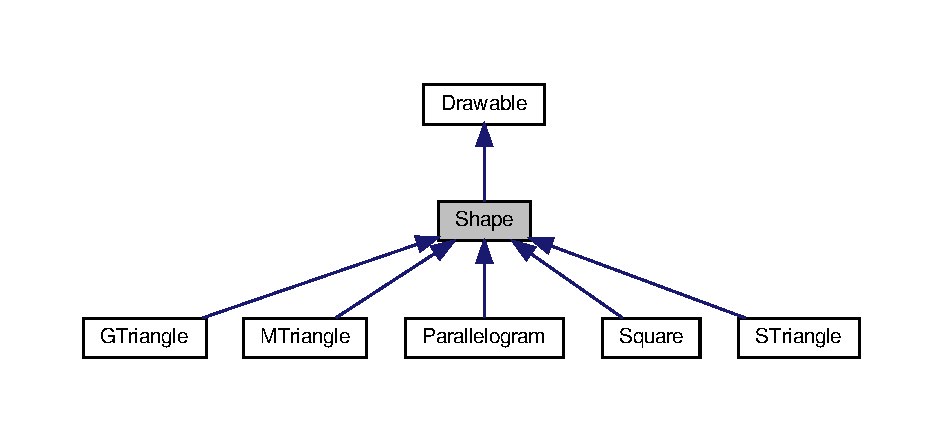
\includegraphics[width=350pt]{classShape__inherit__graph}
\end{center}
\end{figure}


Collaboration diagram for Shape\+:\nopagebreak
\begin{figure}[H]
\begin{center}
\leavevmode
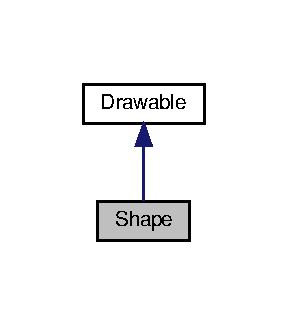
\includegraphics[width=138pt]{classShape__coll__graph}
\end{center}
\end{figure}
\subsection*{Public Member Functions}
\begin{DoxyCompactItemize}
\item 
\mbox{\Hypertarget{classShape_a39fe45638d872f0ce9670d7f85290161}\label{classShape_a39fe45638d872f0ce9670d7f85290161}} 
virtual \hyperlink{classShape_a39fe45638d872f0ce9670d7f85290161}{$\sim$\+Shape} ()=0
\begin{DoxyCompactList}\small\item\em Destructor of Abstract \hyperlink{classShape}{Shape}. \end{DoxyCompactList}\item 
virtual void \hyperlink{classShape_a1f447acd6219cb10b9b7a40371519c46}{move} (const \hyperlink{classPoint}{Point}$<$ double $>$ \&translation)=0
\begin{DoxyCompactList}\small\item\em Pure virtual function. Move the \hyperlink{classShape}{Shape} by point translation. \end{DoxyCompactList}\item 
virtual void \hyperlink{classShape_a2dea8616fd40f2d69fd208715921982a}{rotate} (double angular)=0
\begin{DoxyCompactList}\small\item\em Pure virtual function. Rotate the \hyperlink{classGTriangle}{G\+Triangle} with specified angular. \end{DoxyCompactList}\item 
\mbox{\Hypertarget{classShape_a5a1607f7dc4908225f97aeadb449636d}\label{classShape_a5a1607f7dc4908225f97aeadb449636d}} 
virtual void \hyperlink{classShape_a5a1607f7dc4908225f97aeadb449636d}{flip} ()=0
\begin{DoxyCompactList}\small\item\em Pure virtual function. Flip the figure as symmetry. \end{DoxyCompactList}\item 
virtual bool \hyperlink{classShape_aa09a621da090e42840b4bec7ffb27620}{is\+\_\+in\+\_\+shape} (const \hyperlink{classPoint}{Point}$<$ double $>$ \&point)=0
\begin{DoxyCompactList}\small\item\em Pure virtual function. Check if a point is in this shape. \end{DoxyCompactList}\item 
virtual std\+::vector$<$ \hyperlink{classPoint}{Point}$<$ double $>$ $>$ \hyperlink{classShape_add74a5c682840fa4a519242b1ddbd0b5}{get\+\_\+\+Points} ()=0
\begin{DoxyCompactList}\small\item\em Pure virtual function. Get all points of this shape. \end{DoxyCompactList}\item 
virtual std\+::string \hyperlink{classShape_a98fa87c6dc4c7045fd6897a8f3bc186c}{to\+String} ()=0
\begin{DoxyCompactList}\small\item\em Pure virtual function. Convert all data of \hyperlink{classGTriangle}{G\+Triangle} in a string. \end{DoxyCompactList}\end{DoxyCompactItemize}


\subsection{Detailed Description}
Abstract Class of every \hyperlink{classShape}{Shape}. 

This class manage everything other shape (\hyperlink{classSTriangle}{S\+Triangle}, \hyperlink{classMTriangle}{M\+Triangle}, \hyperlink{classGTriangle}{G\+Triangle}, \hyperlink{classSquare}{Square}, \hyperlink{classParallelogram}{Parallelogram}) 

\subsection{Member Function Documentation}
\mbox{\Hypertarget{classShape_add74a5c682840fa4a519242b1ddbd0b5}\label{classShape_add74a5c682840fa4a519242b1ddbd0b5}} 
\index{Shape@{Shape}!get\+\_\+\+Points@{get\+\_\+\+Points}}
\index{get\+\_\+\+Points@{get\+\_\+\+Points}!Shape@{Shape}}
\subsubsection{\texorpdfstring{get\+\_\+\+Points()}{get\_Points()}}
{\footnotesize\ttfamily virtual std\+::vector$<$\hyperlink{classPoint}{Point}$<$double$>$ $>$ Shape\+::get\+\_\+\+Points (\begin{DoxyParamCaption}{ }\end{DoxyParamCaption})\hspace{0.3cm}{\ttfamily [pure virtual]}}



Pure virtual function. Get all points of this shape. 

\begin{DoxyReturn}{Returns}
Return a vector of points of this shape 
\end{DoxyReturn}


Implemented in \hyperlink{classSTriangle_a08f667453619b506b5c16745a9aa5ecf}{S\+Triangle}, \hyperlink{classGTriangle_add4581d1b52836142de5817de4d52d17}{G\+Triangle}, \hyperlink{classMTriangle_a90351a097a20d35f9d6c4d05ad881e48}{M\+Triangle}, \hyperlink{classParallelogram_a17c9986712806a8b07d90e444e0a543d}{Parallelogram}, and \hyperlink{classSquare_a2a8fb1bfd2f3464cee813ec8b277506e}{Square}.

\mbox{\Hypertarget{classShape_aa09a621da090e42840b4bec7ffb27620}\label{classShape_aa09a621da090e42840b4bec7ffb27620}} 
\index{Shape@{Shape}!is\+\_\+in\+\_\+shape@{is\+\_\+in\+\_\+shape}}
\index{is\+\_\+in\+\_\+shape@{is\+\_\+in\+\_\+shape}!Shape@{Shape}}
\subsubsection{\texorpdfstring{is\+\_\+in\+\_\+shape()}{is\_in\_shape()}}
{\footnotesize\ttfamily virtual bool Shape\+::is\+\_\+in\+\_\+shape (\begin{DoxyParamCaption}\item[{const \hyperlink{classPoint}{Point}$<$ double $>$ \&}]{point }\end{DoxyParamCaption})\hspace{0.3cm}{\ttfamily [pure virtual]}}



Pure virtual function. Check if a point is in this shape. 


\begin{DoxyParams}{Parameters}
{\em point} & \+: \hyperlink{classPoint}{Point} to check \\
\hline
\end{DoxyParams}
\begin{DoxyReturn}{Returns}
true if click is in this shape, false if not 
\end{DoxyReturn}


Implemented in \hyperlink{classSTriangle_a5b55df6eb4af922521da69f69df77b42}{S\+Triangle}, \hyperlink{classGTriangle_abb6f7243155483cc6de301931e87475a}{G\+Triangle}, \hyperlink{classMTriangle_a4cc4cd63537ead67a0b68d1ab25111b4}{M\+Triangle}, \hyperlink{classParallelogram_a585b14ca0f65ed3a5007e8c1df3c6bc4}{Parallelogram}, and \hyperlink{classSquare_ada046df2d9fb92286d106d4b3475980a}{Square}.

\mbox{\Hypertarget{classShape_a1f447acd6219cb10b9b7a40371519c46}\label{classShape_a1f447acd6219cb10b9b7a40371519c46}} 
\index{Shape@{Shape}!move@{move}}
\index{move@{move}!Shape@{Shape}}
\subsubsection{\texorpdfstring{move()}{move()}}
{\footnotesize\ttfamily virtual void Shape\+::move (\begin{DoxyParamCaption}\item[{const \hyperlink{classPoint}{Point}$<$ double $>$ \&}]{translation }\end{DoxyParamCaption})\hspace{0.3cm}{\ttfamily [pure virtual]}}



Pure virtual function. Move the \hyperlink{classShape}{Shape} by point translation. 


\begin{DoxyParams}{Parameters}
{\em translation} & \+: Every points of this shape will be translate by this parameter \\
\hline
\end{DoxyParams}


Implemented in \hyperlink{classSTriangle_ac72888032cde56407193da9435e2fcc0}{S\+Triangle}, \hyperlink{classGTriangle_a6675f3448fca16c1afec576145a9b139}{G\+Triangle}, \hyperlink{classMTriangle_aa21f0514a8af2beba5ecf2ea5a22a4ef}{M\+Triangle}, \hyperlink{classParallelogram_ae8d51f9b629160df31c8a12c28da279e}{Parallelogram}, and \hyperlink{classSquare_a75b2fd22fc3895b83bc20728afb20b10}{Square}.

\mbox{\Hypertarget{classShape_a2dea8616fd40f2d69fd208715921982a}\label{classShape_a2dea8616fd40f2d69fd208715921982a}} 
\index{Shape@{Shape}!rotate@{rotate}}
\index{rotate@{rotate}!Shape@{Shape}}
\subsubsection{\texorpdfstring{rotate()}{rotate()}}
{\footnotesize\ttfamily virtual void Shape\+::rotate (\begin{DoxyParamCaption}\item[{double}]{angular }\end{DoxyParamCaption})\hspace{0.3cm}{\ttfamily [pure virtual]}}



Pure virtual function. Rotate the \hyperlink{classGTriangle}{G\+Triangle} with specified angular. 


\begin{DoxyParams}{Parameters}
{\em angular} & \+: This angular should be between (0, 2\+PI) \\
\hline
\end{DoxyParams}


Implemented in \hyperlink{classGTriangle_ae3ed75bbad4ba7fed68bc06c5834cfbe}{G\+Triangle}, \hyperlink{classMTriangle_a4be29553eeddf99c367b1ec220bc102b}{M\+Triangle}, \hyperlink{classParallelogram_ac498f6a15dea236ecc49bece023d17b0}{Parallelogram}, and \hyperlink{classSquare_a5714e182c30f996b78e74e1badd054a2}{Square}.

\mbox{\Hypertarget{classShape_a98fa87c6dc4c7045fd6897a8f3bc186c}\label{classShape_a98fa87c6dc4c7045fd6897a8f3bc186c}} 
\index{Shape@{Shape}!to\+String@{to\+String}}
\index{to\+String@{to\+String}!Shape@{Shape}}
\subsubsection{\texorpdfstring{to\+String()}{toString()}}
{\footnotesize\ttfamily virtual std\+::string Shape\+::to\+String (\begin{DoxyParamCaption}{ }\end{DoxyParamCaption})\hspace{0.3cm}{\ttfamily [pure virtual]}}



Pure virtual function. Convert all data of \hyperlink{classGTriangle}{G\+Triangle} in a string. 

\begin{DoxyReturn}{Returns}
Return a string which contains every points of this shape 
\end{DoxyReturn}


Implemented in \hyperlink{classSTriangle_a32e4cee65f52d9ee4121c78dc97d86ab}{S\+Triangle}, \hyperlink{classGTriangle_a8381aeea39fac0d52ad9e0d45b791b3b}{G\+Triangle}, \hyperlink{classMTriangle_a7d1fd825592dffa6ac05b3398a8c105a}{M\+Triangle}, \hyperlink{classParallelogram_a9caae0044f23d8a1e87b1a78d852c37f}{Parallelogram}, and \hyperlink{classSquare_aa5d7db8004bba3c400f57513d93b21d4}{Square}.



The documentation for this class was generated from the following files\+:\begin{DoxyCompactItemize}
\item 
include/drawable/\hyperlink{Shape_8hpp}{Shape.\+hpp}\item 
src/drawable/Shape.\+cpp\end{DoxyCompactItemize}

\hypertarget{classSquare}{}\section{Square Class Reference}
\label{classSquare}\index{Square@{Square}}


Class of the square.  




{\ttfamily \#include $<$Square.\+hpp$>$}



Inheritance diagram for Square\+:\nopagebreak
\begin{figure}[H]
\begin{center}
\leavevmode
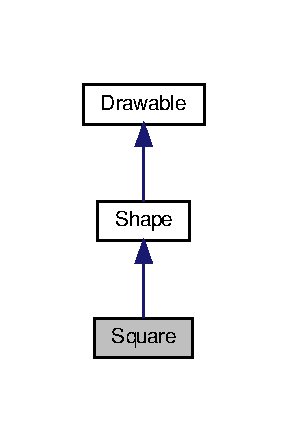
\includegraphics[width=138pt]{classSquare__inherit__graph}
\end{center}
\end{figure}


Collaboration diagram for Square\+:\nopagebreak
\begin{figure}[H]
\begin{center}
\leavevmode
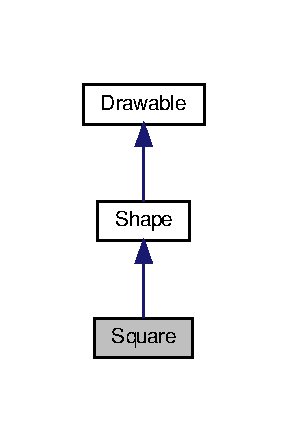
\includegraphics[width=138pt]{classSquare__coll__graph}
\end{center}
\end{figure}
\subsection*{Public Member Functions}
\begin{DoxyCompactItemize}
\item 
\mbox{\Hypertarget{classSquare_ab0677a46d02aa78bc0b7be8c06f9dc37}\label{classSquare_ab0677a46d02aa78bc0b7be8c06f9dc37}} 
\hyperlink{classSquare_ab0677a46d02aa78bc0b7be8c06f9dc37}{$\sim$\+Square} () override
\begin{DoxyCompactList}\small\item\em Destructor of \hyperlink{classSquare}{Square}. \end{DoxyCompactList}\item 
\hyperlink{classSquare_aceff50017f5950b32a967a690213a26e}{Square} (M\+L\+V\+\_\+\+Color color=M\+L\+V\+\_\+\+C\+O\+L\+O\+R\+\_\+\+P\+I\+NK)
\begin{DoxyCompactList}\small\item\em Constructor by default of \hyperlink{classSquare}{Square}, make a \hyperlink{classSquare}{Square} as default. \end{DoxyCompactList}\item 
\hyperlink{classSquare_a6ac91ab99424771ac70670c7973c3f74}{Square} (const std\+::vector$<$ \hyperlink{classSTriangle}{S\+Triangle} $>$ \&triangle, M\+L\+V\+\_\+\+Color color=M\+L\+V\+\_\+\+C\+O\+L\+O\+R\+\_\+\+P\+I\+NK)
\begin{DoxyCompactList}\small\item\em Constructor of \hyperlink{classSquare}{Square}, requires a vector of S\+Triangles. \end{DoxyCompactList}\item 
\hyperlink{classSquare_a80828d5c491e3d76ea4707ddd42685cd}{Square} (const \hyperlink{classPoint}{Point}$<$ double $>$ \&origin, double angular=0.\+0, M\+L\+V\+\_\+\+Color color=M\+L\+V\+\_\+\+C\+O\+L\+O\+R\+\_\+\+P\+I\+NK)
\begin{DoxyCompactList}\small\item\em Constructor of \hyperlink{classSquare}{Square}, calls the deleguate Default Constructor. \end{DoxyCompactList}\item 
void \hyperlink{classSquare_a75b2fd22fc3895b83bc20728afb20b10}{move} (const \hyperlink{classPoint}{Point}$<$ double $>$ \&translation) override
\begin{DoxyCompactList}\small\item\em Move the \hyperlink{classSquare}{Square} by point translation. \end{DoxyCompactList}\item 
void \hyperlink{classSquare_a5714e182c30f996b78e74e1badd054a2}{rotate} (double angular) override
\begin{DoxyCompactList}\small\item\em Rotate the \hyperlink{classSquare}{Square} with specified angular. \end{DoxyCompactList}\item 
\mbox{\Hypertarget{classSquare_a2d56ff842244af8f2fdc85b7e5ce76f3}\label{classSquare_a2d56ff842244af8f2fdc85b7e5ce76f3}} 
void \hyperlink{classSquare_a2d56ff842244af8f2fdc85b7e5ce76f3}{flip} () override
\begin{DoxyCompactList}\small\item\em Flip the figure as symmetry. \end{DoxyCompactList}\item 
\mbox{\Hypertarget{classSquare_a4edbdf9ae0519cc1823f4dbbaa6bbf4c}\label{classSquare_a4edbdf9ae0519cc1823f4dbbaa6bbf4c}} 
void \hyperlink{classSquare_a4edbdf9ae0519cc1823f4dbbaa6bbf4c}{draw} () override
\begin{DoxyCompactList}\small\item\em Draw this shape on I\+HM. \end{DoxyCompactList}\item 
bool \hyperlink{classSquare_ada046df2d9fb92286d106d4b3475980a}{is\+\_\+in\+\_\+shape} (const \hyperlink{classPoint}{Point}$<$ double $>$ \&click) override
\begin{DoxyCompactList}\small\item\em Check if a point is in this shape. \end{DoxyCompactList}\item 
std\+::vector$<$ \hyperlink{classPoint}{Point}$<$ double $>$ $>$ \hyperlink{classSquare_a2a8fb1bfd2f3464cee813ec8b277506e}{get\+\_\+\+Points} () override
\begin{DoxyCompactList}\small\item\em Get points of this shape. \end{DoxyCompactList}\item 
bool \hyperlink{classSquare_ac474644483fa85f7a4f39969f34868fe}{set\+\_\+\+Points} (const \hyperlink{classPoint}{Point}$<$ double $>$ \&ref, const \hyperlink{classPoint}{Point}$<$ double $>$ \&changed) override
\begin{DoxyCompactList}\small\item\em Pure virtual function. Get all points of this shape. \end{DoxyCompactList}\item 
std\+::string \hyperlink{classSquare_aa5d7db8004bba3c400f57513d93b21d4}{to\+String} () override
\begin{DoxyCompactList}\small\item\em Convert all data of \hyperlink{classSquare}{Square} in a string. \end{DoxyCompactList}\end{DoxyCompactItemize}
\subsection*{Additional Inherited Members}


\subsection{Detailed Description}
Class of the square. 

This class manage everything about the \hyperlink{classSquare}{Square} 

\subsection{Constructor \& Destructor Documentation}
\mbox{\Hypertarget{classSquare_aceff50017f5950b32a967a690213a26e}\label{classSquare_aceff50017f5950b32a967a690213a26e}} 
\index{Square@{Square}!Square@{Square}}
\index{Square@{Square}!Square@{Square}}
\subsubsection{\texorpdfstring{Square()}{Square()}\hspace{0.1cm}{\footnotesize\ttfamily [1/3]}}
{\footnotesize\ttfamily Square\+::\+Square (\begin{DoxyParamCaption}\item[{M\+L\+V\+\_\+\+Color}]{color = {\ttfamily MLV\+\_\+COLOR\+\_\+PINK} }\end{DoxyParamCaption})\hspace{0.3cm}{\ttfamily [explicit]}}



Constructor by default of \hyperlink{classSquare}{Square}, make a \hyperlink{classSquare}{Square} as default. 


\begin{DoxyParams}{Parameters}
{\em color} & \+: Optional parameter, color of this shape \\
\hline
\end{DoxyParams}
\mbox{\Hypertarget{classSquare_a6ac91ab99424771ac70670c7973c3f74}\label{classSquare_a6ac91ab99424771ac70670c7973c3f74}} 
\index{Square@{Square}!Square@{Square}}
\index{Square@{Square}!Square@{Square}}
\subsubsection{\texorpdfstring{Square()}{Square()}\hspace{0.1cm}{\footnotesize\ttfamily [2/3]}}
{\footnotesize\ttfamily Square\+::\+Square (\begin{DoxyParamCaption}\item[{const std\+::vector$<$ \hyperlink{classSTriangle}{S\+Triangle} $>$ \&}]{triangle,  }\item[{M\+L\+V\+\_\+\+Color}]{color = {\ttfamily MLV\+\_\+COLOR\+\_\+PINK} }\end{DoxyParamCaption})\hspace{0.3cm}{\ttfamily [explicit]}}



Constructor of \hyperlink{classSquare}{Square}, requires a vector of S\+Triangles. 


\begin{DoxyParams}{Parameters}
{\em triangle} & \+: The \hyperlink{classSquare}{Square} will created with a vector of \hyperlink{classSTriangle}{S\+Triangle} (4) \\
\hline
{\em color} & \+: Optional parameter, color of this shape \\
\hline
\end{DoxyParams}
\mbox{\Hypertarget{classSquare_a80828d5c491e3d76ea4707ddd42685cd}\label{classSquare_a80828d5c491e3d76ea4707ddd42685cd}} 
\index{Square@{Square}!Square@{Square}}
\index{Square@{Square}!Square@{Square}}
\subsubsection{\texorpdfstring{Square()}{Square()}\hspace{0.1cm}{\footnotesize\ttfamily [3/3]}}
{\footnotesize\ttfamily Square\+::\+Square (\begin{DoxyParamCaption}\item[{const \hyperlink{classPoint}{Point}$<$ double $>$ \&}]{origin,  }\item[{double}]{angular = {\ttfamily 0.0},  }\item[{M\+L\+V\+\_\+\+Color}]{color = {\ttfamily MLV\+\_\+COLOR\+\_\+PINK} }\end{DoxyParamCaption})\hspace{0.3cm}{\ttfamily [explicit]}}



Constructor of \hyperlink{classSquare}{Square}, calls the deleguate Default Constructor. 


\begin{DoxyParams}{Parameters}
{\em origin} & \+: shifts the figure of a translation of the origin \\
\hline
{\em angular} & \+: Optional parameter (angular=0.\+0 as default), rotate the figure with an angular \\
\hline
{\em color} & \+: Optional parameter, color of this shape \\
\hline
\end{DoxyParams}


\subsection{Member Function Documentation}
\mbox{\Hypertarget{classSquare_a2a8fb1bfd2f3464cee813ec8b277506e}\label{classSquare_a2a8fb1bfd2f3464cee813ec8b277506e}} 
\index{Square@{Square}!get\+\_\+\+Points@{get\+\_\+\+Points}}
\index{get\+\_\+\+Points@{get\+\_\+\+Points}!Square@{Square}}
\subsubsection{\texorpdfstring{get\+\_\+\+Points()}{get\_Points()}}
{\footnotesize\ttfamily std\+::vector$<$ \hyperlink{classPoint}{Point}$<$ double $>$ $>$ Square\+::get\+\_\+\+Points (\begin{DoxyParamCaption}{ }\end{DoxyParamCaption})\hspace{0.3cm}{\ttfamily [override]}, {\ttfamily [virtual]}}



Get points of this shape. 

\begin{DoxyReturn}{Returns}
Return a vector of points of this shape 
\end{DoxyReturn}


Implements \hyperlink{classShape_add74a5c682840fa4a519242b1ddbd0b5}{Shape}.

\mbox{\Hypertarget{classSquare_ada046df2d9fb92286d106d4b3475980a}\label{classSquare_ada046df2d9fb92286d106d4b3475980a}} 
\index{Square@{Square}!is\+\_\+in\+\_\+shape@{is\+\_\+in\+\_\+shape}}
\index{is\+\_\+in\+\_\+shape@{is\+\_\+in\+\_\+shape}!Square@{Square}}
\subsubsection{\texorpdfstring{is\+\_\+in\+\_\+shape()}{is\_in\_shape()}}
{\footnotesize\ttfamily bool Square\+::is\+\_\+in\+\_\+shape (\begin{DoxyParamCaption}\item[{const \hyperlink{classPoint}{Point}$<$ double $>$ \&}]{click }\end{DoxyParamCaption})\hspace{0.3cm}{\ttfamily [override]}, {\ttfamily [virtual]}}



Check if a point is in this shape. 


\begin{DoxyParams}{Parameters}
{\em click} & \+: \hyperlink{classPoint}{Point} to check \\
\hline
\end{DoxyParams}
\begin{DoxyReturn}{Returns}
true if click is in this shape, false if not 
\end{DoxyReturn}


Implements \hyperlink{classShape_aa09a621da090e42840b4bec7ffb27620}{Shape}.

\mbox{\Hypertarget{classSquare_a75b2fd22fc3895b83bc20728afb20b10}\label{classSquare_a75b2fd22fc3895b83bc20728afb20b10}} 
\index{Square@{Square}!move@{move}}
\index{move@{move}!Square@{Square}}
\subsubsection{\texorpdfstring{move()}{move()}}
{\footnotesize\ttfamily void Square\+::move (\begin{DoxyParamCaption}\item[{const \hyperlink{classPoint}{Point}$<$ double $>$ \&}]{translation }\end{DoxyParamCaption})\hspace{0.3cm}{\ttfamily [override]}, {\ttfamily [virtual]}}



Move the \hyperlink{classSquare}{Square} by point translation. 


\begin{DoxyParams}{Parameters}
{\em translation} & \+: Every points of this shape will be translate by this parameter \\
\hline
\end{DoxyParams}


Implements \hyperlink{classShape_a1f447acd6219cb10b9b7a40371519c46}{Shape}.

\mbox{\Hypertarget{classSquare_a5714e182c30f996b78e74e1badd054a2}\label{classSquare_a5714e182c30f996b78e74e1badd054a2}} 
\index{Square@{Square}!rotate@{rotate}}
\index{rotate@{rotate}!Square@{Square}}
\subsubsection{\texorpdfstring{rotate()}{rotate()}}
{\footnotesize\ttfamily void Square\+::rotate (\begin{DoxyParamCaption}\item[{double}]{angular }\end{DoxyParamCaption})\hspace{0.3cm}{\ttfamily [override]}, {\ttfamily [virtual]}}



Rotate the \hyperlink{classSquare}{Square} with specified angular. 


\begin{DoxyParams}{Parameters}
{\em angular} & \+: This angular should be between (0, 2\+PI) \\
\hline
\end{DoxyParams}


Implements \hyperlink{classShape_a2dea8616fd40f2d69fd208715921982a}{Shape}.

\mbox{\Hypertarget{classSquare_ac474644483fa85f7a4f39969f34868fe}\label{classSquare_ac474644483fa85f7a4f39969f34868fe}} 
\index{Square@{Square}!set\+\_\+\+Points@{set\+\_\+\+Points}}
\index{set\+\_\+\+Points@{set\+\_\+\+Points}!Square@{Square}}
\subsubsection{\texorpdfstring{set\+\_\+\+Points()}{set\_Points()}}
{\footnotesize\ttfamily bool Square\+::set\+\_\+\+Points (\begin{DoxyParamCaption}\item[{const \hyperlink{classPoint}{Point}$<$ double $>$ \&}]{ref,  }\item[{const \hyperlink{classPoint}{Point}$<$ double $>$ \&}]{changed }\end{DoxyParamCaption})\hspace{0.3cm}{\ttfamily [override]}, {\ttfamily [virtual]}}



Pure virtual function. Get all points of this shape. 

\begin{DoxyReturn}{Returns}
Return a vector of points of this shape 
\end{DoxyReturn}


Implements \hyperlink{classShape_a6eb0d80cccc44cb72b06c61d9780bc6b}{Shape}.

\mbox{\Hypertarget{classSquare_aa5d7db8004bba3c400f57513d93b21d4}\label{classSquare_aa5d7db8004bba3c400f57513d93b21d4}} 
\index{Square@{Square}!to\+String@{to\+String}}
\index{to\+String@{to\+String}!Square@{Square}}
\subsubsection{\texorpdfstring{to\+String()}{toString()}}
{\footnotesize\ttfamily std\+::string Square\+::to\+String (\begin{DoxyParamCaption}{ }\end{DoxyParamCaption})\hspace{0.3cm}{\ttfamily [override]}, {\ttfamily [virtual]}}



Convert all data of \hyperlink{classSquare}{Square} in a string. 

\begin{DoxyReturn}{Returns}
Return a string which contains every points of this shape 
\end{DoxyReturn}


Implements \hyperlink{classShape_a98fa87c6dc4c7045fd6897a8f3bc186c}{Shape}.



The documentation for this class was generated from the following files\+:\begin{DoxyCompactItemize}
\item 
include/shape/\hyperlink{Square_8hpp}{Square.\+hpp}\item 
src/shape/Square.\+cpp\end{DoxyCompactItemize}

\hypertarget{classSTriangle}{}\section{S\+Triangle Class Reference}
\label{classSTriangle}\index{S\+Triangle@{S\+Triangle}}


Class of the small triangle.  




{\ttfamily \#include $<$S\+Triangle.\+hpp$>$}



Inheritance diagram for S\+Triangle\+:\nopagebreak
\begin{figure}[H]
\begin{center}
\leavevmode
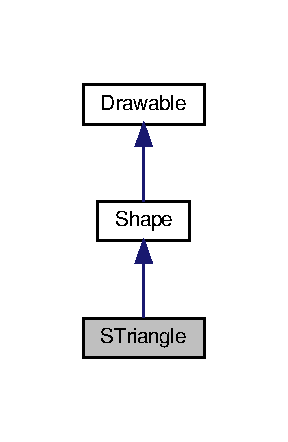
\includegraphics[width=138pt]{classSTriangle__inherit__graph}
\end{center}
\end{figure}


Collaboration diagram for S\+Triangle\+:\nopagebreak
\begin{figure}[H]
\begin{center}
\leavevmode
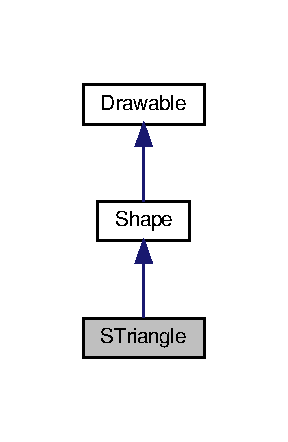
\includegraphics[width=138pt]{classSTriangle__coll__graph}
\end{center}
\end{figure}
\subsection*{Public Member Functions}
\begin{DoxyCompactItemize}
\item 
\mbox{\Hypertarget{classSTriangle_ad278fb75870a545bcb6617058c77d73f}\label{classSTriangle_ad278fb75870a545bcb6617058c77d73f}} 
\hyperlink{classSTriangle_ad278fb75870a545bcb6617058c77d73f}{$\sim$\+S\+Triangle} () override
\begin{DoxyCompactList}\small\item\em Destructor of \hyperlink{classSTriangle}{S\+Triangle}. \end{DoxyCompactList}\item 
\hyperlink{classSTriangle_a56ad36f53fbb46fb05d57ca6e4a41f2a}{S\+Triangle} (M\+L\+V\+\_\+\+Color color=M\+L\+V\+\_\+\+C\+O\+L\+O\+R\+\_\+\+G\+R\+E\+EN)
\begin{DoxyCompactList}\small\item\em Constructor by default of \hyperlink{classMTriangle}{M\+Triangle}, make a \hyperlink{classSTriangle}{S\+Triangle} as default. \end{DoxyCompactList}\item 
\hyperlink{classSTriangle_a2f80f360d80efc87dfdbbdd555d1ecfe}{S\+Triangle} (const \hyperlink{classPoint}{Point}$<$ double $>$ \&p1, const \hyperlink{classPoint}{Point}$<$ double $>$ \&p2, const \hyperlink{classPoint}{Point}$<$ double $>$ \&p3, M\+L\+V\+\_\+\+Color color=M\+L\+V\+\_\+\+C\+O\+L\+O\+R\+\_\+\+G\+R\+E\+EN)
\begin{DoxyCompactList}\small\item\em Constructor of \hyperlink{classSTriangle}{S\+Triangle}, requires 3 points. \end{DoxyCompactList}\item 
\hyperlink{classSTriangle_ad22ceb26e87756cdbe432e8adf743b55}{S\+Triangle} (const std\+::vector$<$ \hyperlink{classPoint}{Point}$<$ double $>$$>$ \&points, M\+L\+V\+\_\+\+Color color=M\+L\+V\+\_\+\+C\+O\+L\+O\+R\+\_\+\+G\+R\+E\+EN)
\begin{DoxyCompactList}\small\item\em Constructor of \hyperlink{classSTriangle}{S\+Triangle}, requires a vector of 3 points. \end{DoxyCompactList}\item 
\hyperlink{classSTriangle_af5129d1631bf4d546921c7e3758fe905}{S\+Triangle} (const \hyperlink{classPoint}{Point}$<$ double $>$ \&origin, double angular=0.\+0, M\+L\+V\+\_\+\+Color color=M\+L\+V\+\_\+\+C\+O\+L\+O\+R\+\_\+\+G\+R\+E\+EN)
\begin{DoxyCompactList}\small\item\em Constructor of \hyperlink{classSTriangle}{S\+Triangle}, calls the deleguate Default Constructor. \end{DoxyCompactList}\item 
void \hyperlink{classSTriangle_ac72888032cde56407193da9435e2fcc0}{move} (const \hyperlink{classPoint}{Point}$<$ double $>$ \&translation) override
\begin{DoxyCompactList}\small\item\em Move the \hyperlink{classMTriangle}{M\+Triangle} by point translation. \end{DoxyCompactList}\item 
void \hyperlink{classSTriangle_a53b7f48c2bc66402170912686e77ec5d}{rotate} (double angular, const \hyperlink{classPoint}{Point}$<$ double $>$ \&center\+\_\+point)
\begin{DoxyCompactList}\small\item\em Rotate an \hyperlink{classSTriangle}{S\+Triangle} with specified angular, used only for an other shape. \end{DoxyCompactList}\item 
\mbox{\Hypertarget{classSTriangle_af16f2a83efc6d94578e2feb560983850}\label{classSTriangle_af16f2a83efc6d94578e2feb560983850}} 
void \hyperlink{classSTriangle_af16f2a83efc6d94578e2feb560983850}{flip} () override
\begin{DoxyCompactList}\small\item\em Flip the figure as symmetry. \end{DoxyCompactList}\item 
\mbox{\Hypertarget{classSTriangle_aacf293108989708da341b1fbaeee0aca}\label{classSTriangle_aacf293108989708da341b1fbaeee0aca}} 
void \hyperlink{classSTriangle_aacf293108989708da341b1fbaeee0aca}{draw} () override
\begin{DoxyCompactList}\small\item\em Draw this shape on I\+HM. \end{DoxyCompactList}\item 
void \hyperlink{classSTriangle_a7eddfc5b9e5b2951ba71b085345d87d1}{draw} (M\+L\+V\+\_\+\+Color Color)
\begin{DoxyCompactList}\small\item\em Draw this shape on I\+HM with specific color. \end{DoxyCompactList}\item 
bool \hyperlink{classSTriangle_a5b55df6eb4af922521da69f69df77b42}{is\+\_\+in\+\_\+shape} (const \hyperlink{classPoint}{Point}$<$ double $>$ \&click) override
\begin{DoxyCompactList}\small\item\em Check if a point is in this shape. \end{DoxyCompactList}\item 
bool \hyperlink{classSTriangle_a6824246f68484d8d8159a3315df257a4}{is\+\_\+in\+\_\+triangle} (const \hyperlink{classPoint}{Point}$<$ double $>$ \&click)
\begin{DoxyCompactList}\small\item\em Check if a point is in this \hyperlink{classSTriangle}{S\+Triangle}. \end{DoxyCompactList}\item 
std\+::string \hyperlink{classSTriangle_a32e4cee65f52d9ee4121c78dc97d86ab}{to\+String} () override
\begin{DoxyCompactList}\small\item\em Convert all data of \hyperlink{classMTriangle}{M\+Triangle} in a string. \end{DoxyCompactList}\item 
std\+::vector$<$ \hyperlink{classPoint}{Point}$<$ double $>$ $>$ \hyperlink{classSTriangle_a08f667453619b506b5c16745a9aa5ecf}{get\+\_\+\+Points} () override
\begin{DoxyCompactList}\small\item\em Get every points of this \hyperlink{classSTriangle}{S\+Triangle}. \end{DoxyCompactList}\item 
bool \hyperlink{classSTriangle_acab6926951bd8f2558e4c658610c0e51}{set\+\_\+\+Points} (const \hyperlink{classPoint}{Point}$<$ double $>$ \&ref, const \hyperlink{classPoint}{Point}$<$ double $>$ \&changed) override
\begin{DoxyCompactList}\small\item\em Pure virtual function. Get all points of this shape. \end{DoxyCompactList}\item 
\hyperlink{classPoint}{Point}$<$ double $>$ \hyperlink{classSTriangle_a61228a7f80ee90de80dff8c4e046f51f}{get\+\_\+center\+\_\+point} ()
\begin{DoxyCompactList}\small\item\em Get the current center point of this \hyperlink{classSTriangle}{S\+Triangle}. \end{DoxyCompactList}\end{DoxyCompactItemize}
\subsection*{Static Public Member Functions}
\begin{DoxyCompactItemize}
\item 
static \hyperlink{classPoint}{Point}$<$ double $>$ \hyperlink{classSTriangle_ac8e4d59ebc85924650597a181045e2a0}{center\+\_\+point} (const std\+::vector$<$ \hyperlink{classPoint}{Point}$<$ double $>$$>$ \&list\+\_\+points)
\begin{DoxyCompactList}\small\item\em Compute the center point of N points. \end{DoxyCompactList}\end{DoxyCompactItemize}


\subsection{Detailed Description}
Class of the small triangle. 

This class manage everything about the small triangle 

\subsection{Constructor \& Destructor Documentation}
\mbox{\Hypertarget{classSTriangle_a56ad36f53fbb46fb05d57ca6e4a41f2a}\label{classSTriangle_a56ad36f53fbb46fb05d57ca6e4a41f2a}} 
\index{S\+Triangle@{S\+Triangle}!S\+Triangle@{S\+Triangle}}
\index{S\+Triangle@{S\+Triangle}!S\+Triangle@{S\+Triangle}}
\subsubsection{\texorpdfstring{S\+Triangle()}{STriangle()}\hspace{0.1cm}{\footnotesize\ttfamily [1/4]}}
{\footnotesize\ttfamily S\+Triangle\+::\+S\+Triangle (\begin{DoxyParamCaption}\item[{M\+L\+V\+\_\+\+Color}]{color = {\ttfamily MLV\+\_\+COLOR\+\_\+GREEN} }\end{DoxyParamCaption})\hspace{0.3cm}{\ttfamily [explicit]}}



Constructor by default of \hyperlink{classMTriangle}{M\+Triangle}, make a \hyperlink{classSTriangle}{S\+Triangle} as default. 


\begin{DoxyParams}{Parameters}
{\em color} & \+: Optional parameter, color of this shape \\
\hline
\end{DoxyParams}
\mbox{\Hypertarget{classSTriangle_a2f80f360d80efc87dfdbbdd555d1ecfe}\label{classSTriangle_a2f80f360d80efc87dfdbbdd555d1ecfe}} 
\index{S\+Triangle@{S\+Triangle}!S\+Triangle@{S\+Triangle}}
\index{S\+Triangle@{S\+Triangle}!S\+Triangle@{S\+Triangle}}
\subsubsection{\texorpdfstring{S\+Triangle()}{STriangle()}\hspace{0.1cm}{\footnotesize\ttfamily [2/4]}}
{\footnotesize\ttfamily S\+Triangle\+::\+S\+Triangle (\begin{DoxyParamCaption}\item[{const \hyperlink{classPoint}{Point}$<$ double $>$ \&}]{p1,  }\item[{const \hyperlink{classPoint}{Point}$<$ double $>$ \&}]{p2,  }\item[{const \hyperlink{classPoint}{Point}$<$ double $>$ \&}]{p3,  }\item[{M\+L\+V\+\_\+\+Color}]{color = {\ttfamily MLV\+\_\+COLOR\+\_\+GREEN} }\end{DoxyParamCaption})}



Constructor of \hyperlink{classSTriangle}{S\+Triangle}, requires 3 points. 


\begin{DoxyParams}{Parameters}
{\em p1} & \+: First point of the \hyperlink{classSTriangle}{S\+Triangle} \\
\hline
{\em p2} & \+: Second point of the \hyperlink{classSTriangle}{S\+Triangle} \\
\hline
{\em p3} & \+: Third point of the \hyperlink{classSTriangle}{S\+Triangle} \\
\hline
{\em color} & \+: Optional parameter, color of this shape \\
\hline
\end{DoxyParams}
\mbox{\Hypertarget{classSTriangle_ad22ceb26e87756cdbe432e8adf743b55}\label{classSTriangle_ad22ceb26e87756cdbe432e8adf743b55}} 
\index{S\+Triangle@{S\+Triangle}!S\+Triangle@{S\+Triangle}}
\index{S\+Triangle@{S\+Triangle}!S\+Triangle@{S\+Triangle}}
\subsubsection{\texorpdfstring{S\+Triangle()}{STriangle()}\hspace{0.1cm}{\footnotesize\ttfamily [3/4]}}
{\footnotesize\ttfamily S\+Triangle\+::\+S\+Triangle (\begin{DoxyParamCaption}\item[{const std\+::vector$<$ \hyperlink{classPoint}{Point}$<$ double $>$$>$ \&}]{points,  }\item[{M\+L\+V\+\_\+\+Color}]{color = {\ttfamily MLV\+\_\+COLOR\+\_\+GREEN} }\end{DoxyParamCaption})\hspace{0.3cm}{\ttfamily [explicit]}}



Constructor of \hyperlink{classSTriangle}{S\+Triangle}, requires a vector of 3 points. 


\begin{DoxyParams}{Parameters}
{\em points} & \+: vector of 3 points \\
\hline
{\em color} & \+: Optional parameter, color of this shape \\
\hline
\end{DoxyParams}
\mbox{\Hypertarget{classSTriangle_af5129d1631bf4d546921c7e3758fe905}\label{classSTriangle_af5129d1631bf4d546921c7e3758fe905}} 
\index{S\+Triangle@{S\+Triangle}!S\+Triangle@{S\+Triangle}}
\index{S\+Triangle@{S\+Triangle}!S\+Triangle@{S\+Triangle}}
\subsubsection{\texorpdfstring{S\+Triangle()}{STriangle()}\hspace{0.1cm}{\footnotesize\ttfamily [4/4]}}
{\footnotesize\ttfamily S\+Triangle\+::\+S\+Triangle (\begin{DoxyParamCaption}\item[{const \hyperlink{classPoint}{Point}$<$ double $>$ \&}]{origin,  }\item[{double}]{angular = {\ttfamily 0.0},  }\item[{M\+L\+V\+\_\+\+Color}]{color = {\ttfamily MLV\+\_\+COLOR\+\_\+GREEN} }\end{DoxyParamCaption})\hspace{0.3cm}{\ttfamily [explicit]}}



Constructor of \hyperlink{classSTriangle}{S\+Triangle}, calls the deleguate Default Constructor. 


\begin{DoxyParams}{Parameters}
{\em origin} & \+: shifts the figure of a translation of the origin \\
\hline
{\em angular} & \+: Optional parameter (angular=0.\+0 as default), rotate the figure with an angular \\
\hline
{\em color} & \+: Optional parameter, color of this shape \\
\hline
\end{DoxyParams}


\subsection{Member Function Documentation}
\mbox{\Hypertarget{classSTriangle_ac8e4d59ebc85924650597a181045e2a0}\label{classSTriangle_ac8e4d59ebc85924650597a181045e2a0}} 
\index{S\+Triangle@{S\+Triangle}!center\+\_\+point@{center\+\_\+point}}
\index{center\+\_\+point@{center\+\_\+point}!S\+Triangle@{S\+Triangle}}
\subsubsection{\texorpdfstring{center\+\_\+point()}{center\_point()}}
{\footnotesize\ttfamily \hyperlink{classPoint}{Point}$<$ double $>$ S\+Triangle\+::center\+\_\+point (\begin{DoxyParamCaption}\item[{const std\+::vector$<$ \hyperlink{classPoint}{Point}$<$ double $>$$>$ \&}]{list\+\_\+points }\end{DoxyParamCaption})\hspace{0.3cm}{\ttfamily [static]}}



Compute the center point of N points. 


\begin{DoxyParams}{Parameters}
{\em list\+\_\+points} & \+: vector of N points \\
\hline
\end{DoxyParams}
\begin{DoxyReturn}{Returns}
Return the center point of these N points 
\end{DoxyReturn}
\mbox{\Hypertarget{classSTriangle_a7eddfc5b9e5b2951ba71b085345d87d1}\label{classSTriangle_a7eddfc5b9e5b2951ba71b085345d87d1}} 
\index{S\+Triangle@{S\+Triangle}!draw@{draw}}
\index{draw@{draw}!S\+Triangle@{S\+Triangle}}
\subsubsection{\texorpdfstring{draw()}{draw()}}
{\footnotesize\ttfamily void S\+Triangle\+::draw (\begin{DoxyParamCaption}\item[{M\+L\+V\+\_\+\+Color}]{Color }\end{DoxyParamCaption})}



Draw this shape on I\+HM with specific color. 


\begin{DoxyParams}{Parameters}
{\em Color} & \+: Color from the graphic library M\+LV like M\+L\+V\+\_\+\+C\+O\+L\+O\+R\+\_\+\+X\+XX \\
\hline
\end{DoxyParams}
\mbox{\Hypertarget{classSTriangle_a61228a7f80ee90de80dff8c4e046f51f}\label{classSTriangle_a61228a7f80ee90de80dff8c4e046f51f}} 
\index{S\+Triangle@{S\+Triangle}!get\+\_\+center\+\_\+point@{get\+\_\+center\+\_\+point}}
\index{get\+\_\+center\+\_\+point@{get\+\_\+center\+\_\+point}!S\+Triangle@{S\+Triangle}}
\subsubsection{\texorpdfstring{get\+\_\+center\+\_\+point()}{get\_center\_point()}}
{\footnotesize\ttfamily \hyperlink{classPoint}{Point}$<$ double $>$ S\+Triangle\+::get\+\_\+center\+\_\+point (\begin{DoxyParamCaption}{ }\end{DoxyParamCaption})}



Get the current center point of this \hyperlink{classSTriangle}{S\+Triangle}. 

\begin{DoxyReturn}{Returns}
Return the current center point of this \hyperlink{classSTriangle}{S\+Triangle} 
\end{DoxyReturn}
\mbox{\Hypertarget{classSTriangle_a08f667453619b506b5c16745a9aa5ecf}\label{classSTriangle_a08f667453619b506b5c16745a9aa5ecf}} 
\index{S\+Triangle@{S\+Triangle}!get\+\_\+\+Points@{get\+\_\+\+Points}}
\index{get\+\_\+\+Points@{get\+\_\+\+Points}!S\+Triangle@{S\+Triangle}}
\subsubsection{\texorpdfstring{get\+\_\+\+Points()}{get\_Points()}}
{\footnotesize\ttfamily std\+::vector$<$ \hyperlink{classPoint}{Point}$<$ double $>$ $>$ S\+Triangle\+::get\+\_\+\+Points (\begin{DoxyParamCaption}{ }\end{DoxyParamCaption})\hspace{0.3cm}{\ttfamily [override]}, {\ttfamily [virtual]}}



Get every points of this \hyperlink{classSTriangle}{S\+Triangle}. 

\begin{DoxyReturn}{Returns}
Return a vector of these points 
\end{DoxyReturn}


Implements \hyperlink{classShape_add74a5c682840fa4a519242b1ddbd0b5}{Shape}.

\mbox{\Hypertarget{classSTriangle_a5b55df6eb4af922521da69f69df77b42}\label{classSTriangle_a5b55df6eb4af922521da69f69df77b42}} 
\index{S\+Triangle@{S\+Triangle}!is\+\_\+in\+\_\+shape@{is\+\_\+in\+\_\+shape}}
\index{is\+\_\+in\+\_\+shape@{is\+\_\+in\+\_\+shape}!S\+Triangle@{S\+Triangle}}
\subsubsection{\texorpdfstring{is\+\_\+in\+\_\+shape()}{is\_in\_shape()}}
{\footnotesize\ttfamily bool S\+Triangle\+::is\+\_\+in\+\_\+shape (\begin{DoxyParamCaption}\item[{const \hyperlink{classPoint}{Point}$<$ double $>$ \&}]{click }\end{DoxyParamCaption})\hspace{0.3cm}{\ttfamily [override]}, {\ttfamily [virtual]}}



Check if a point is in this shape. 


\begin{DoxyParams}{Parameters}
{\em click} & \+: \hyperlink{classPoint}{Point} to check \\
\hline
\end{DoxyParams}
\begin{DoxyReturn}{Returns}
true if click is in this shape, false if not 
\end{DoxyReturn}


Implements \hyperlink{classShape_aa09a621da090e42840b4bec7ffb27620}{Shape}.

\mbox{\Hypertarget{classSTriangle_a6824246f68484d8d8159a3315df257a4}\label{classSTriangle_a6824246f68484d8d8159a3315df257a4}} 
\index{S\+Triangle@{S\+Triangle}!is\+\_\+in\+\_\+triangle@{is\+\_\+in\+\_\+triangle}}
\index{is\+\_\+in\+\_\+triangle@{is\+\_\+in\+\_\+triangle}!S\+Triangle@{S\+Triangle}}
\subsubsection{\texorpdfstring{is\+\_\+in\+\_\+triangle()}{is\_in\_triangle()}}
{\footnotesize\ttfamily bool S\+Triangle\+::is\+\_\+in\+\_\+triangle (\begin{DoxyParamCaption}\item[{const \hyperlink{classPoint}{Point}$<$ double $>$ \&}]{click }\end{DoxyParamCaption})}



Check if a point is in this \hyperlink{classSTriangle}{S\+Triangle}. 


\begin{DoxyParams}{Parameters}
{\em click} & \+: \hyperlink{classPoint}{Point} to check \\
\hline
\end{DoxyParams}
\begin{DoxyReturn}{Returns}
true if click is in this shape, false if not 
\end{DoxyReturn}
\mbox{\Hypertarget{classSTriangle_ac72888032cde56407193da9435e2fcc0}\label{classSTriangle_ac72888032cde56407193da9435e2fcc0}} 
\index{S\+Triangle@{S\+Triangle}!move@{move}}
\index{move@{move}!S\+Triangle@{S\+Triangle}}
\subsubsection{\texorpdfstring{move()}{move()}}
{\footnotesize\ttfamily void S\+Triangle\+::move (\begin{DoxyParamCaption}\item[{const \hyperlink{classPoint}{Point}$<$ double $>$ \&}]{translation }\end{DoxyParamCaption})\hspace{0.3cm}{\ttfamily [override]}, {\ttfamily [virtual]}}



Move the \hyperlink{classMTriangle}{M\+Triangle} by point translation. 


\begin{DoxyParams}{Parameters}
{\em translation} & \+: Every points of this shape will be translate by this parameter \\
\hline
\end{DoxyParams}


Implements \hyperlink{classShape_a1f447acd6219cb10b9b7a40371519c46}{Shape}.

\mbox{\Hypertarget{classSTriangle_a53b7f48c2bc66402170912686e77ec5d}\label{classSTriangle_a53b7f48c2bc66402170912686e77ec5d}} 
\index{S\+Triangle@{S\+Triangle}!rotate@{rotate}}
\index{rotate@{rotate}!S\+Triangle@{S\+Triangle}}
\subsubsection{\texorpdfstring{rotate()}{rotate()}}
{\footnotesize\ttfamily void S\+Triangle\+::rotate (\begin{DoxyParamCaption}\item[{double}]{angular,  }\item[{const \hyperlink{classPoint}{Point}$<$ double $>$ \&}]{center\+\_\+point }\end{DoxyParamCaption})}



Rotate an \hyperlink{classSTriangle}{S\+Triangle} with specified angular, used only for an other shape. 


\begin{DoxyParams}{Parameters}
{\em angular} & \+: This angular should be between (0, 2\+PI) \\
\hline
{\em center\+\_\+point} & \+: Rotate an \hyperlink{classSTriangle}{S\+Triangle} around this point \\
\hline
\end{DoxyParams}
\mbox{\Hypertarget{classSTriangle_acab6926951bd8f2558e4c658610c0e51}\label{classSTriangle_acab6926951bd8f2558e4c658610c0e51}} 
\index{S\+Triangle@{S\+Triangle}!set\+\_\+\+Points@{set\+\_\+\+Points}}
\index{set\+\_\+\+Points@{set\+\_\+\+Points}!S\+Triangle@{S\+Triangle}}
\subsubsection{\texorpdfstring{set\+\_\+\+Points()}{set\_Points()}}
{\footnotesize\ttfamily bool S\+Triangle\+::set\+\_\+\+Points (\begin{DoxyParamCaption}\item[{const \hyperlink{classPoint}{Point}$<$ double $>$ \&}]{ref,  }\item[{const \hyperlink{classPoint}{Point}$<$ double $>$ \&}]{changed }\end{DoxyParamCaption})\hspace{0.3cm}{\ttfamily [override]}, {\ttfamily [virtual]}}



Pure virtual function. Get all points of this shape. 

\begin{DoxyReturn}{Returns}
Return a vector of points of this shape 
\end{DoxyReturn}


Implements \hyperlink{classShape_a6eb0d80cccc44cb72b06c61d9780bc6b}{Shape}.

\mbox{\Hypertarget{classSTriangle_a32e4cee65f52d9ee4121c78dc97d86ab}\label{classSTriangle_a32e4cee65f52d9ee4121c78dc97d86ab}} 
\index{S\+Triangle@{S\+Triangle}!to\+String@{to\+String}}
\index{to\+String@{to\+String}!S\+Triangle@{S\+Triangle}}
\subsubsection{\texorpdfstring{to\+String()}{toString()}}
{\footnotesize\ttfamily std\+::string S\+Triangle\+::to\+String (\begin{DoxyParamCaption}{ }\end{DoxyParamCaption})\hspace{0.3cm}{\ttfamily [override]}, {\ttfamily [virtual]}}



Convert all data of \hyperlink{classMTriangle}{M\+Triangle} in a string. 

\begin{DoxyReturn}{Returns}
Return a string which contains every points of this shape 
\end{DoxyReturn}


Implements \hyperlink{classShape_a98fa87c6dc4c7045fd6897a8f3bc186c}{Shape}.



The documentation for this class was generated from the following files\+:\begin{DoxyCompactItemize}
\item 
include/shape/\hyperlink{STriangle_8hpp}{S\+Triangle.\+hpp}\item 
src/shape/S\+Triangle.\+cpp\end{DoxyCompactItemize}

\chapter{File Documentation}
\hypertarget{Button_8hpp}{}\section{include/drawable/\+Button.hpp File Reference}
\label{Button_8hpp}\index{include/drawable/\+Button.\+hpp@{include/drawable/\+Button.\+hpp}}


Every buttons of menu.  


{\ttfamily \#include $<$utility$>$}\newline
{\ttfamily \#include $<$utils/\+Point.\+hpp$>$}\newline
{\ttfamily \#include $<$functional$>$}\newline
Include dependency graph for Button.\+hpp\+:
\nopagebreak
\begin{figure}[H]
\begin{center}
\leavevmode
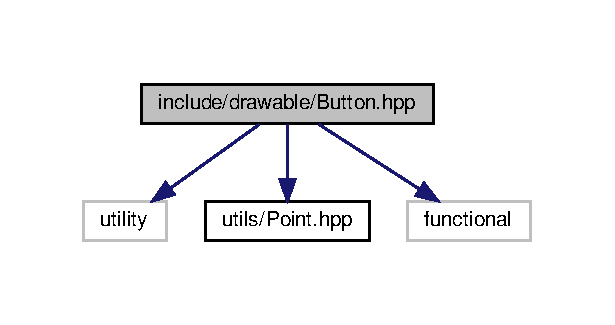
\includegraphics[width=295pt]{Button_8hpp__incl}
\end{center}
\end{figure}
This graph shows which files directly or indirectly include this file\+:
\nopagebreak
\begin{figure}[H]
\begin{center}
\leavevmode
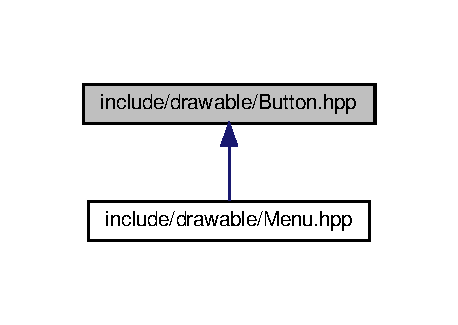
\includegraphics[width=220pt]{Button_8hpp__dep__incl}
\end{center}
\end{figure}
\subsection*{Classes}
\begin{DoxyCompactItemize}
\item 
class \hyperlink{classButton}{Button}
\begin{DoxyCompactList}\small\item\em \hyperlink{classButton}{Button} of the \hyperlink{classMenu}{Menu}. \end{DoxyCompactList}\end{DoxyCompactItemize}


\subsection{Detailed Description}
Every buttons of menu. 

\begin{DoxyAuthor}{Author}
Jérémie LE B\+A\+S\+T\+A\+RD 
\end{DoxyAuthor}
\begin{DoxyVersion}{Version}
1.\+0 
\end{DoxyVersion}

\hypertarget{Menu_8hpp}{}\section{include/drawable/\+Menu.hpp File Reference}
\label{Menu_8hpp}\index{include/drawable/\+Menu.\+hpp@{include/drawable/\+Menu.\+hpp}}


\hyperlink{classMenu}{Menu} of the Tangram\textquotesingle{}s \hyperlink{classGame}{Game}.  


{\ttfamily \#include $<$drawable/\+Button.\+hpp$>$}\newline
{\ttfamily \#include $<$vector$>$}\newline
Include dependency graph for Menu.\+hpp\+:\nopagebreak
\begin{figure}[H]
\begin{center}
\leavevmode
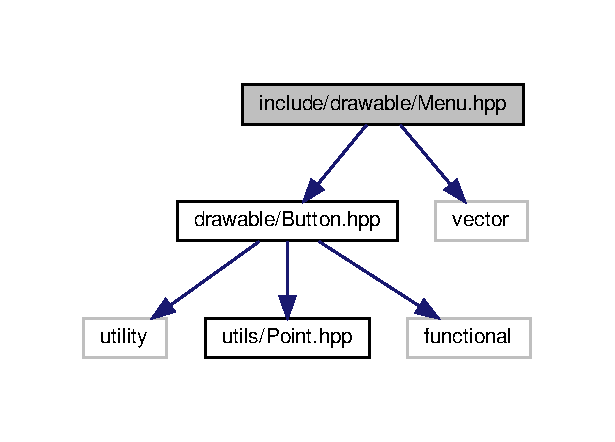
\includegraphics[width=295pt]{Menu_8hpp__incl}
\end{center}
\end{figure}
\subsection*{Classes}
\begin{DoxyCompactItemize}
\item 
class \hyperlink{classMenu}{Menu}
\begin{DoxyCompactList}\small\item\em \hyperlink{classMenu}{Menu} of the game. \end{DoxyCompactList}\end{DoxyCompactItemize}


\subsection{Detailed Description}
\hyperlink{classMenu}{Menu} of the Tangram\textquotesingle{}s \hyperlink{classGame}{Game}. 

\begin{DoxyAuthor}{Author}
Jérémie LE B\+A\+S\+T\+A\+RD 
\end{DoxyAuthor}
\begin{DoxyVersion}{Version}
1.\+0 
\end{DoxyVersion}

\hypertarget{Shape_8hpp}{}\section{include/drawable/\+Shape.hpp File Reference}
\label{Shape_8hpp}\index{include/drawable/\+Shape.\+hpp@{include/drawable/\+Shape.\+hpp}}


Abstract Class \hyperlink{classShape}{Shape} of every shape in Tangram.  


{\ttfamily \#include $<$vector$>$}\newline
{\ttfamily \#include $<$string$>$}\newline
{\ttfamily \#include $<$utils/\+Point.\+hpp$>$}\newline
{\ttfamily \#include $<$drawable/\+Drawable.\+h$>$}\newline
Include dependency graph for Shape.\+hpp\+:
\nopagebreak
\begin{figure}[H]
\begin{center}
\leavevmode
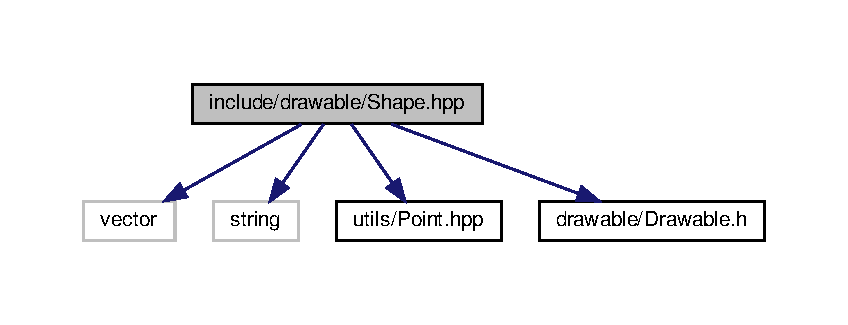
\includegraphics[width=350pt]{Shape_8hpp__incl}
\end{center}
\end{figure}
This graph shows which files directly or indirectly include this file\+:
\nopagebreak
\begin{figure}[H]
\begin{center}
\leavevmode
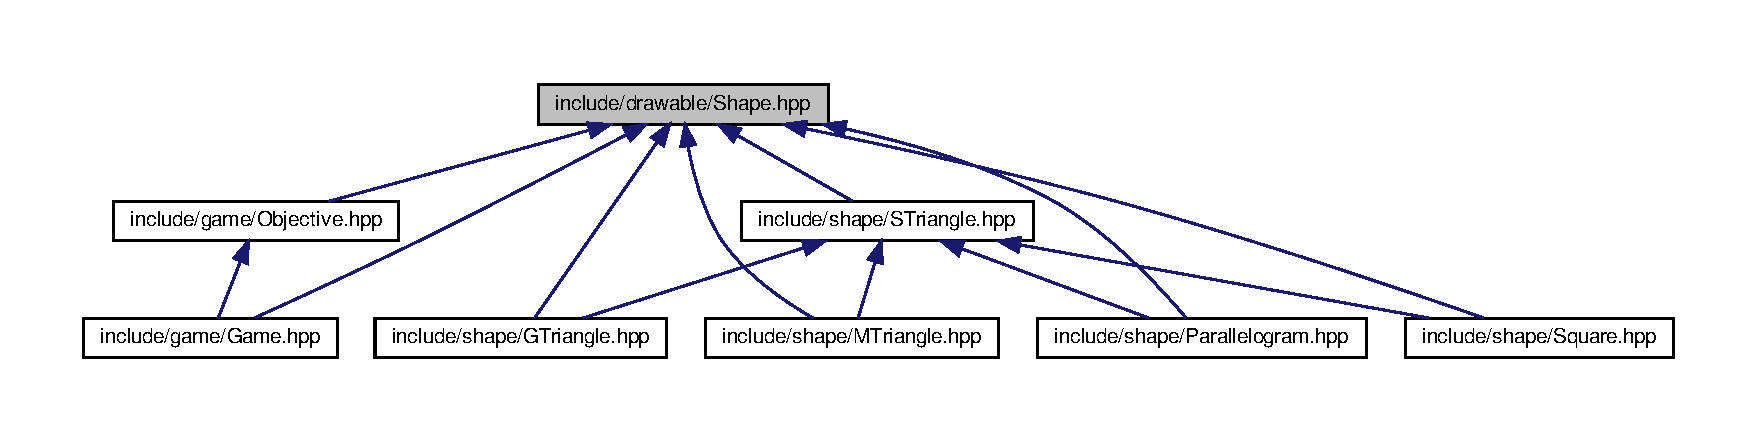
\includegraphics[width=350pt]{Shape_8hpp__dep__incl}
\end{center}
\end{figure}
\subsection*{Classes}
\begin{DoxyCompactItemize}
\item 
class \hyperlink{classShape}{Shape}
\begin{DoxyCompactList}\small\item\em Abstract Class of every \hyperlink{classShape}{Shape}. \end{DoxyCompactList}\end{DoxyCompactItemize}


\subsection{Detailed Description}
Abstract Class \hyperlink{classShape}{Shape} of every shape in Tangram. 

\begin{DoxyAuthor}{Author}
Jérémie LE B\+A\+S\+T\+A\+RD 
\end{DoxyAuthor}
\begin{DoxyVersion}{Version}
1.\+0 
\end{DoxyVersion}

\hypertarget{Game_8hpp}{}\section{include/game/\+Game.hpp File Reference}
\label{Game_8hpp}\index{include/game/\+Game.\+hpp@{include/game/\+Game.\+hpp}}


Main \hyperlink{classGame}{Game} of the Tangram.  


{\ttfamily \#include $<$game/\+Objective.\+hpp$>$}\newline
{\ttfamily \#include $<$drawable/\+Shape.\+hpp$>$}\newline
Include dependency graph for Game.\+hpp\+:
\nopagebreak
\begin{figure}[H]
\begin{center}
\leavevmode
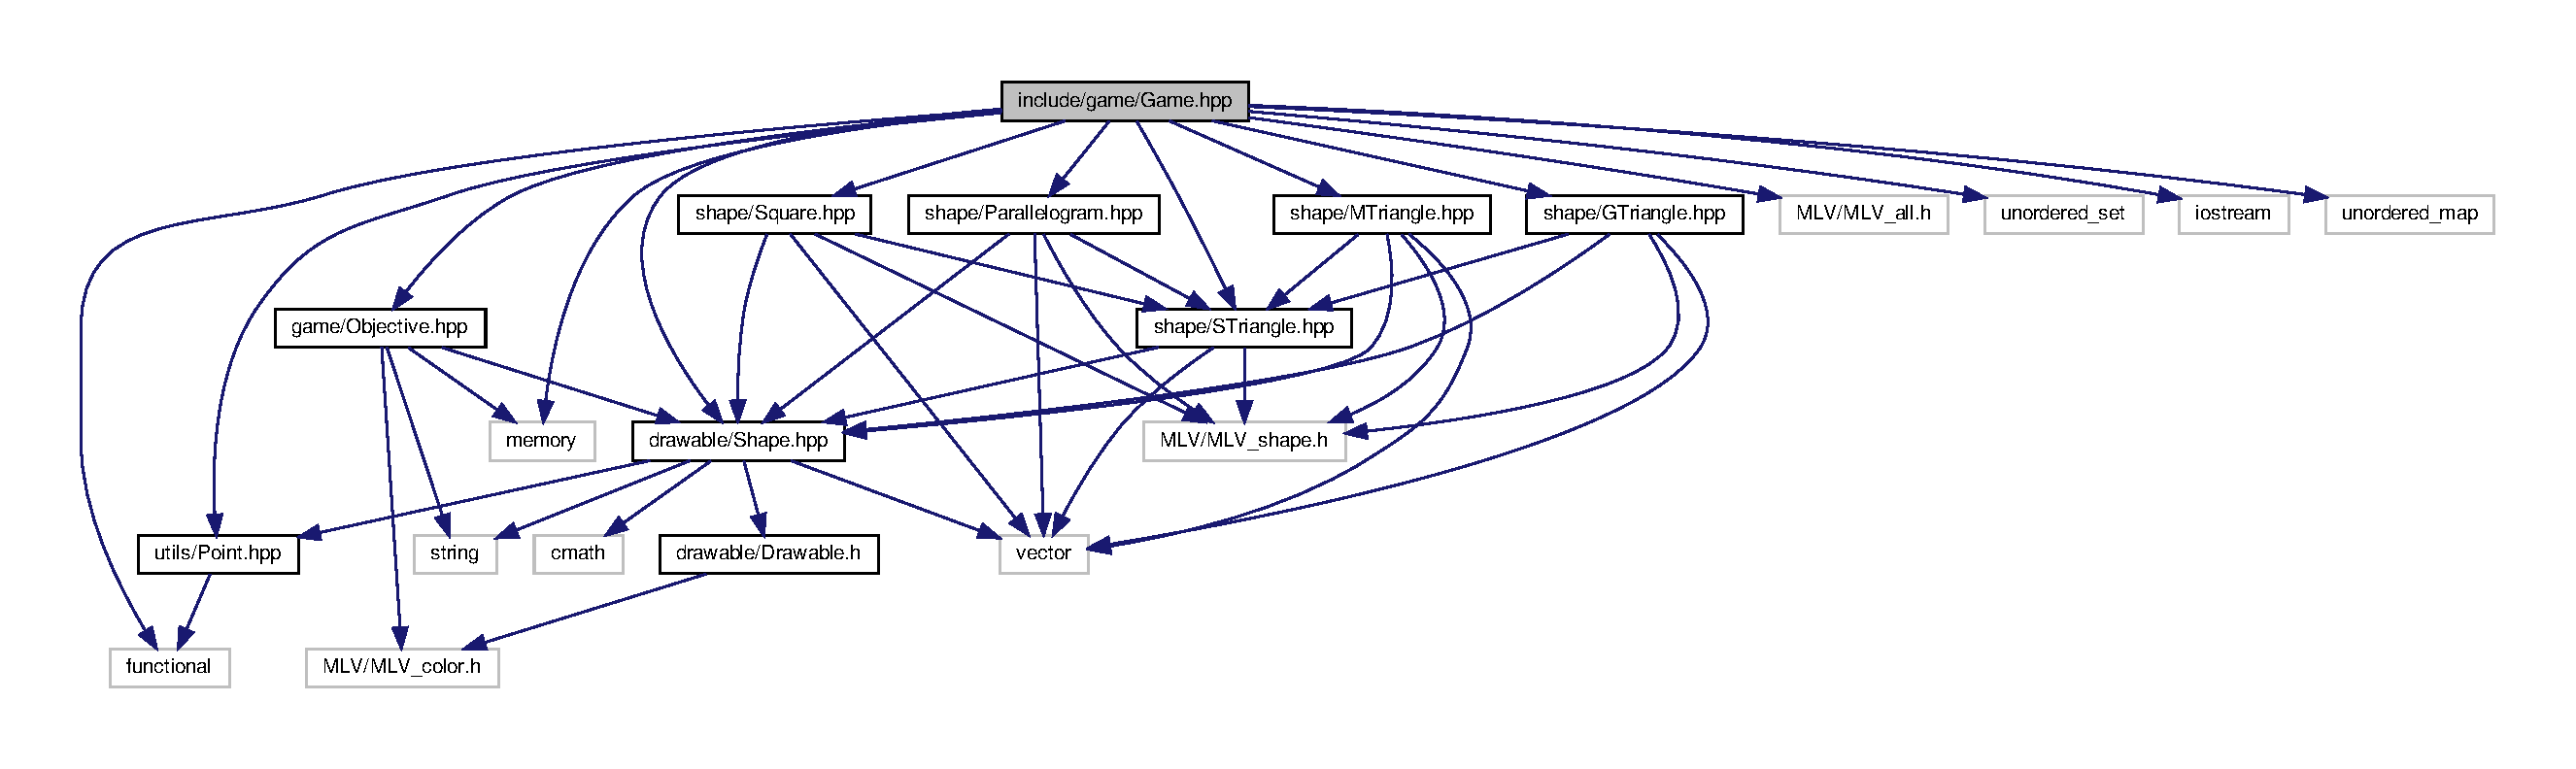
\includegraphics[width=350pt]{Game_8hpp__incl}
\end{center}
\end{figure}
This graph shows which files directly or indirectly include this file\+:
\nopagebreak
\begin{figure}[H]
\begin{center}
\leavevmode
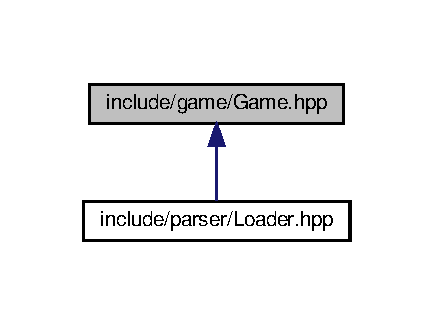
\includegraphics[width=208pt]{Game_8hpp__dep__incl}
\end{center}
\end{figure}
\subsection*{Classes}
\begin{DoxyCompactItemize}
\item 
class \hyperlink{classGame}{Game}
\begin{DoxyCompactList}\small\item\em Class of the main \hyperlink{classGame}{Game}. \end{DoxyCompactList}\end{DoxyCompactItemize}


\subsection{Detailed Description}
Main \hyperlink{classGame}{Game} of the Tangram. 

\begin{DoxyAuthor}{Author}
Jérémie LE B\+A\+S\+T\+A\+RD 
\end{DoxyAuthor}
\begin{DoxyVersion}{Version}
1.\+0 
\end{DoxyVersion}

\hypertarget{Objective_8hpp}{}\section{include/game/\+Objective.hpp File Reference}
\label{Objective_8hpp}\index{include/game/\+Objective.\+hpp@{include/game/\+Objective.\+hpp}}


\hyperlink{classObjective}{Objective} of the Tangram\textquotesingle{}s board.  


{\ttfamily \#include $<$drawable/\+Shape.\+hpp$>$}\newline
Include dependency graph for Objective.\+hpp\+:\nopagebreak
\begin{figure}[H]
\begin{center}
\leavevmode
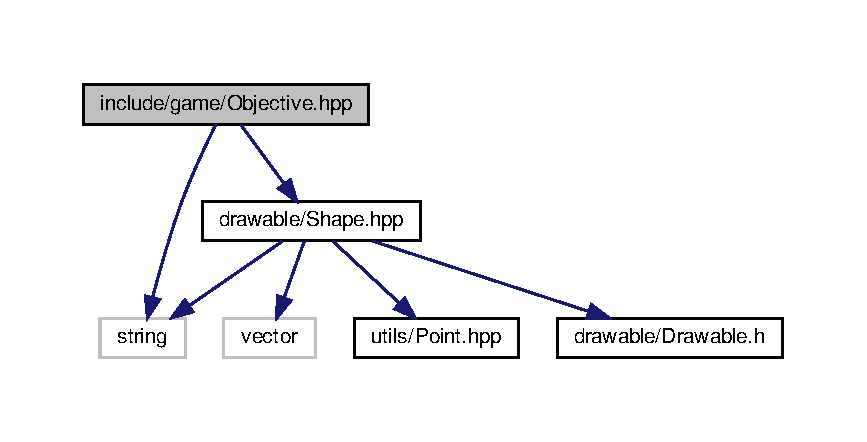
\includegraphics[width=348pt]{Objective_8hpp__incl}
\end{center}
\end{figure}
This graph shows which files directly or indirectly include this file\+:\nopagebreak
\begin{figure}[H]
\begin{center}
\leavevmode
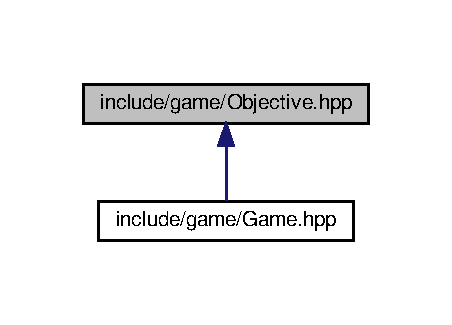
\includegraphics[width=217pt]{Objective_8hpp__dep__incl}
\end{center}
\end{figure}
\subsection*{Classes}
\begin{DoxyCompactItemize}
\item 
class \hyperlink{classObjective}{Objective}
\begin{DoxyCompactList}\small\item\em Class of the board \hyperlink{classObjective}{Objective}. \end{DoxyCompactList}\end{DoxyCompactItemize}


\subsection{Detailed Description}
\hyperlink{classObjective}{Objective} of the Tangram\textquotesingle{}s board. 

\begin{DoxyAuthor}{Author}
Jérémie LE B\+A\+S\+T\+A\+RD 
\end{DoxyAuthor}
\begin{DoxyVersion}{Version}
1.\+0 
\end{DoxyVersion}

\hypertarget{Loader_8hpp}{}\section{include/parser/\+Loader.hpp File Reference}
\label{Loader_8hpp}\index{include/parser/\+Loader.\+hpp@{include/parser/\+Loader.\+hpp}}


Load a board of Tangram.  


{\ttfamily \#include $<$game/\+Game.\+hpp$>$}\newline
{\ttfamily \#include $<$filesystem$>$}\newline
Include dependency graph for Loader.\+hpp\+:\nopagebreak
\begin{figure}[H]
\begin{center}
\leavevmode
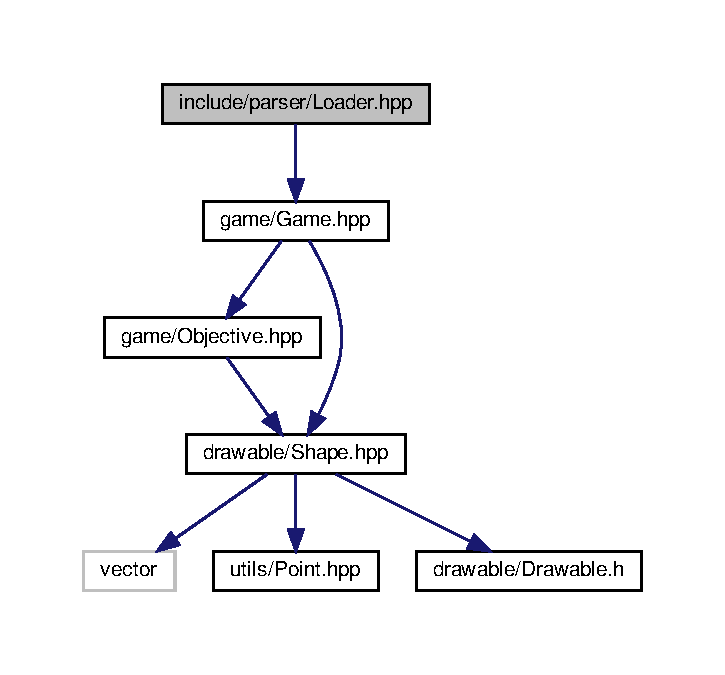
\includegraphics[width=350pt]{Loader_8hpp__incl}
\end{center}
\end{figure}
\subsection*{Classes}
\begin{DoxyCompactItemize}
\item 
class \hyperlink{classLoader}{Loader}
\begin{DoxyCompactList}\small\item\em Class of the main \hyperlink{classLoader}{Loader}. \end{DoxyCompactList}\end{DoxyCompactItemize}


\subsection{Detailed Description}
Load a board of Tangram. 

\begin{DoxyAuthor}{Author}
Jérémie LE B\+A\+S\+T\+A\+RD 
\end{DoxyAuthor}
\begin{DoxyVersion}{Version}
1.\+0 
\end{DoxyVersion}

\hypertarget{Save_8hpp}{}\section{include/parser/\+C_Save.hpp File Reference}
\label{Save_8hpp}\index{include/parser/\+C_Save.\+hpp@{include/parser/\+C_Save.\+hpp}}


\hyperlink{classSave}{C_Save} a board of Tangram.


\subsection*{Classes}
\begin{DoxyCompactItemize}
\item 
class \hyperlink{classSave}{C_Save}
\begin{DoxyCompactList}\small\item\em Class of the main Saver. \end{DoxyCompactList}\end{DoxyCompactItemize}


\subsection{Detailed Description}
\hyperlink{classSave}{C_Save} a board of Tangram.

\begin{DoxyAuthor}{Author}
Jérémie LE B\+A\+S\+T\+A\+RD 
\end{DoxyAuthor}
\begin{DoxyVersion}{Version}
1.\+0 
\end{DoxyVersion}

\hypertarget{GTriangle_8hpp}{}\section{include/shape/\+G\+Triangle.hpp File Reference}
\label{GTriangle_8hpp}\index{include/shape/\+G\+Triangle.\+hpp@{include/shape/\+G\+Triangle.\+hpp}}


\hyperlink{classShape}{Shape} of Great Triangle.  


{\ttfamily \#include $<$vector$>$}\newline
{\ttfamily \#include $<$shape/\+S\+Triangle.\+hpp$>$}\newline
{\ttfamily \#include $<$drawable/\+Shape.\+hpp$>$}\newline
{\ttfamily \#include $<$M\+L\+V/\+M\+L\+V\+\_\+shape.\+h$>$}\newline
Include dependency graph for G\+Triangle.\+hpp\+:
\nopagebreak
\begin{figure}[H]
\begin{center}
\leavevmode
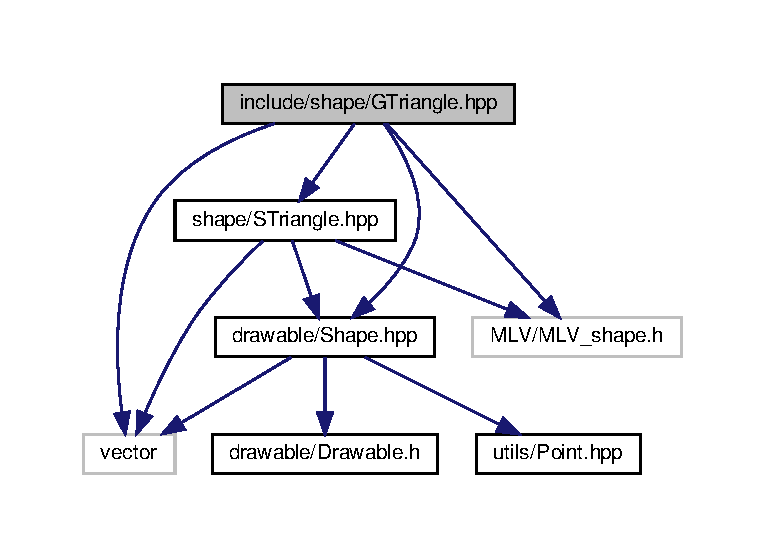
\includegraphics[width=350pt]{GTriangle_8hpp__incl}
\end{center}
\end{figure}
This graph shows which files directly or indirectly include this file\+:
\nopagebreak
\begin{figure}[H]
\begin{center}
\leavevmode
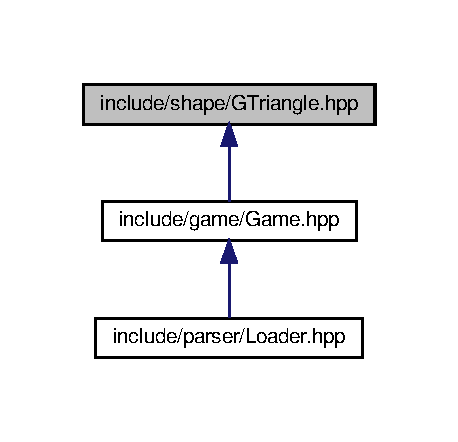
\includegraphics[width=220pt]{GTriangle_8hpp__dep__incl}
\end{center}
\end{figure}
\subsection*{Classes}
\begin{DoxyCompactItemize}
\item 
class \hyperlink{classGTriangle}{G\+Triangle}
\begin{DoxyCompactList}\small\item\em Class of the greatest triangle. \end{DoxyCompactList}\end{DoxyCompactItemize}


\subsection{Detailed Description}
\hyperlink{classShape}{Shape} of Great Triangle. 

\begin{DoxyAuthor}{Author}
Jérémie LE B\+A\+S\+T\+A\+RD 
\end{DoxyAuthor}
\begin{DoxyVersion}{Version}
1.\+0 
\end{DoxyVersion}

\hypertarget{MTriangle_8hpp}{}\section{include/shape/\+M\+Triangle.hpp File Reference}
\label{MTriangle_8hpp}\index{include/shape/\+M\+Triangle.\+hpp@{include/shape/\+M\+Triangle.\+hpp}}


\hyperlink{classShape}{A_Shape} of Medium Triangle.


{\ttfamily \#include $<$vector$>$}\newline
{\ttfamily \#include $<$shape/\+S\+Triangle.\+hpp$>$}\newline
{\ttfamily \#include $<$drawable/\+A_Shape.\+hpp$>$}\newline
{\ttfamily \#include $<$M\+L\+V/\+M\+L\+V\+\_\+shape.\+h$>$}\newline
Include dependency graph for M\+Triangle.\+hpp\+:
\nopagebreak
\begin{figure}[H]
\begin{center}
\leavevmode
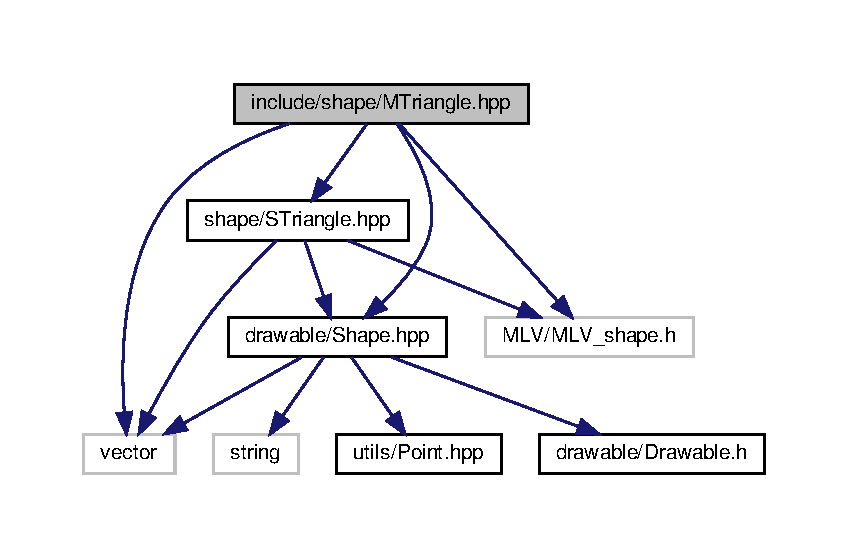
\includegraphics[width=350pt]{MTriangle_8hpp__incl}
\end{center}
\end{figure}
This graph shows which files directly or indirectly include this file\+:
\nopagebreak
\begin{figure}[H]
\begin{center}
\leavevmode
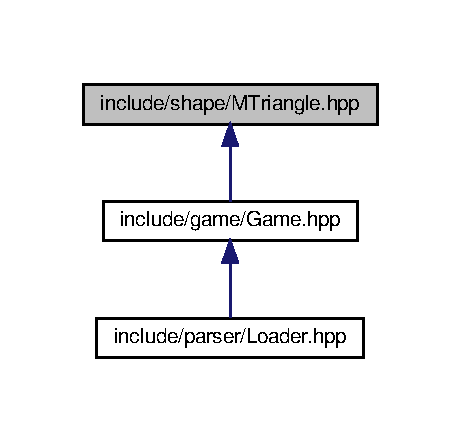
\includegraphics[width=221pt]{MTriangle_8hpp__dep__incl}
\end{center}
\end{figure}
\subsection*{Classes}
\begin{DoxyCompactItemize}
\item 
class \hyperlink{classMTriangle}{M\+Triangle}
\begin{DoxyCompactList}\small\item\em Class of the medium mTriangles. \end{DoxyCompactList}\end{DoxyCompactItemize}


\subsection{Detailed Description}
\hyperlink{classShape}{A_Shape} of Medium Triangle.

\begin{DoxyAuthor}{Author}
Jérémie LE B\+A\+S\+T\+A\+RD 
\end{DoxyAuthor}
\begin{DoxyVersion}{Version}
1.\+0 
\end{DoxyVersion}

\hypertarget{Parallelogram_8hpp}{}\section{include/shape/\+Parallelogram.hpp File Reference}
\label{Parallelogram_8hpp}\index{include/shape/\+Parallelogram.\+hpp@{include/shape/\+Parallelogram.\+hpp}}


\hyperlink{classShape}{Shape} of \hyperlink{classParallelogram}{Parallelogram}.  


{\ttfamily \#include $<$vector$>$}\newline
{\ttfamily \#include $<$shape/\+S\+Triangle.\+hpp$>$}\newline
{\ttfamily \#include $<$drawable/\+Shape.\+hpp$>$}\newline
{\ttfamily \#include $<$M\+L\+V/\+M\+L\+V\+\_\+shape.\+h$>$}\newline
Include dependency graph for Parallelogram.\+hpp\+:\nopagebreak
\begin{figure}[H]
\begin{center}
\leavevmode
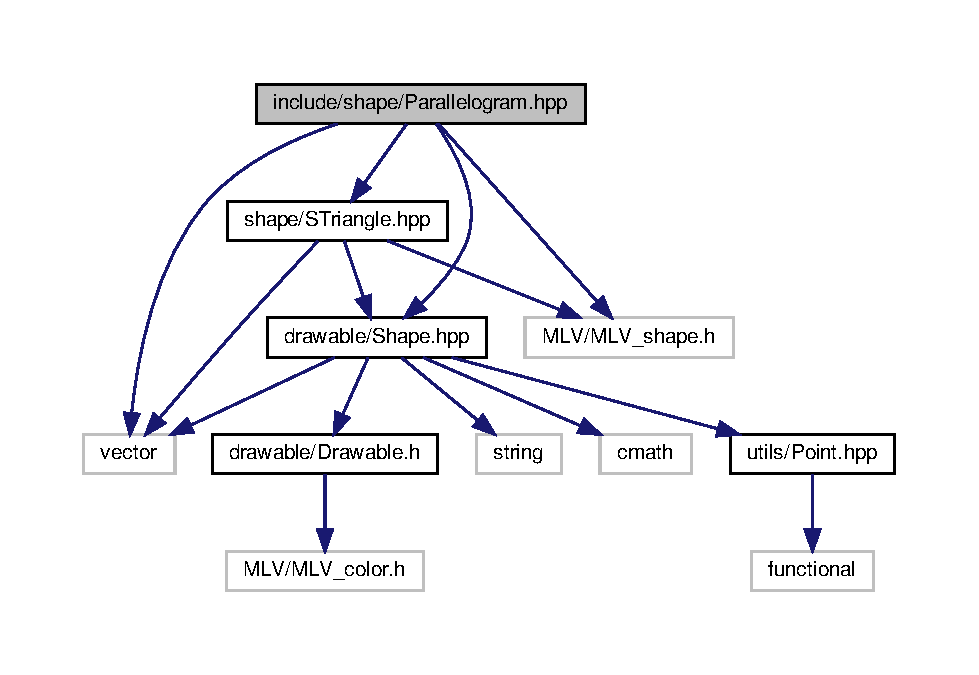
\includegraphics[width=350pt]{Parallelogram_8hpp__incl}
\end{center}
\end{figure}
\subsection*{Classes}
\begin{DoxyCompactItemize}
\item 
class \hyperlink{classParallelogram}{Parallelogram}
\begin{DoxyCompactList}\small\item\em Class of the parallelogram. \end{DoxyCompactList}\end{DoxyCompactItemize}


\subsection{Detailed Description}
\hyperlink{classShape}{Shape} of \hyperlink{classParallelogram}{Parallelogram}. 

\begin{DoxyAuthor}{Author}
Jérémie LE B\+A\+S\+T\+A\+RD 
\end{DoxyAuthor}
\begin{DoxyVersion}{Version}
1.\+0 
\end{DoxyVersion}

\hypertarget{Square_8hpp}{}\section{include/shape/\+Square.hpp File Reference}
\label{Square_8hpp}\index{include/shape/\+Square.\+hpp@{include/shape/\+Square.\+hpp}}


\hyperlink{classShape}{Shape} of \hyperlink{classSquare}{Square}.  


{\ttfamily \#include $<$vector$>$}\newline
{\ttfamily \#include $<$shape/\+S\+Triangle.\+hpp$>$}\newline
{\ttfamily \#include $<$drawable/\+Shape.\+hpp$>$}\newline
{\ttfamily \#include $<$M\+L\+V/\+M\+L\+V\+\_\+shape.\+h$>$}\newline
Include dependency graph for Square.\+hpp\+:\nopagebreak
\begin{figure}[H]
\begin{center}
\leavevmode
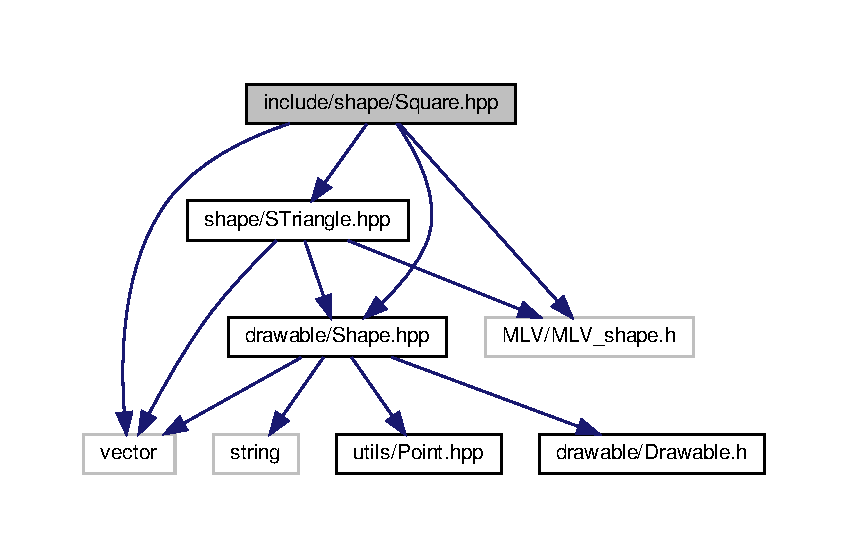
\includegraphics[width=350pt]{Square_8hpp__incl}
\end{center}
\end{figure}
\subsection*{Classes}
\begin{DoxyCompactItemize}
\item 
class \hyperlink{classSquare}{Square}
\begin{DoxyCompactList}\small\item\em Class of the square. \end{DoxyCompactList}\end{DoxyCompactItemize}


\subsection{Detailed Description}
\hyperlink{classShape}{Shape} of \hyperlink{classSquare}{Square}. 

\begin{DoxyAuthor}{Author}
Jérémie LE B\+A\+S\+T\+A\+RD 
\end{DoxyAuthor}
\begin{DoxyVersion}{Version}
1.\+0 
\end{DoxyVersion}

\hypertarget{STriangle_8hpp}{}\section{include/shape/\+S\+Triangle.hpp File Reference}
\label{STriangle_8hpp}\index{include/shape/\+S\+Triangle.\+hpp@{include/shape/\+S\+Triangle.\+hpp}}


\hyperlink{classShape}{A_Shape} of Small Triangle.


{\ttfamily \#include $<$vector$>$}\newline
{\ttfamily \#include $<$drawable/\+A_Shape.\+hpp$>$}\newline
{\ttfamily \#include $<$M\+L\+V/\+M\+L\+V\+\_\+shape.\+h$>$}\newline
Include dependency graph for S\+Triangle.\+hpp\+:
\nopagebreak
\begin{figure}[H]
\begin{center}
\leavevmode
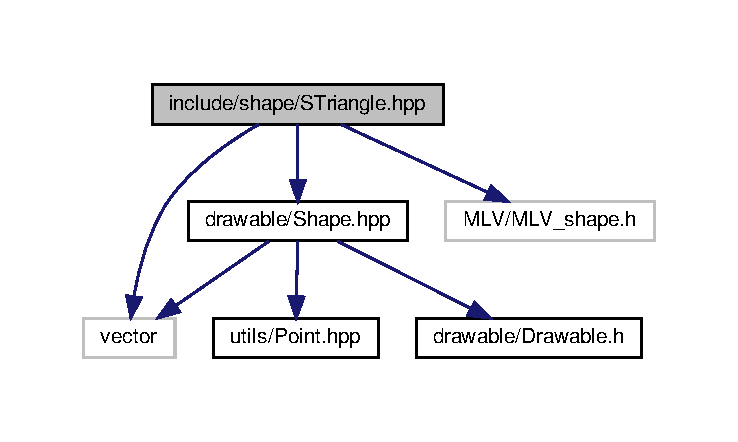
\includegraphics[width=350pt]{STriangle_8hpp__incl}
\end{center}
\end{figure}
This graph shows which files directly or indirectly include this file\+:
\nopagebreak
\begin{figure}[H]
\begin{center}
\leavevmode
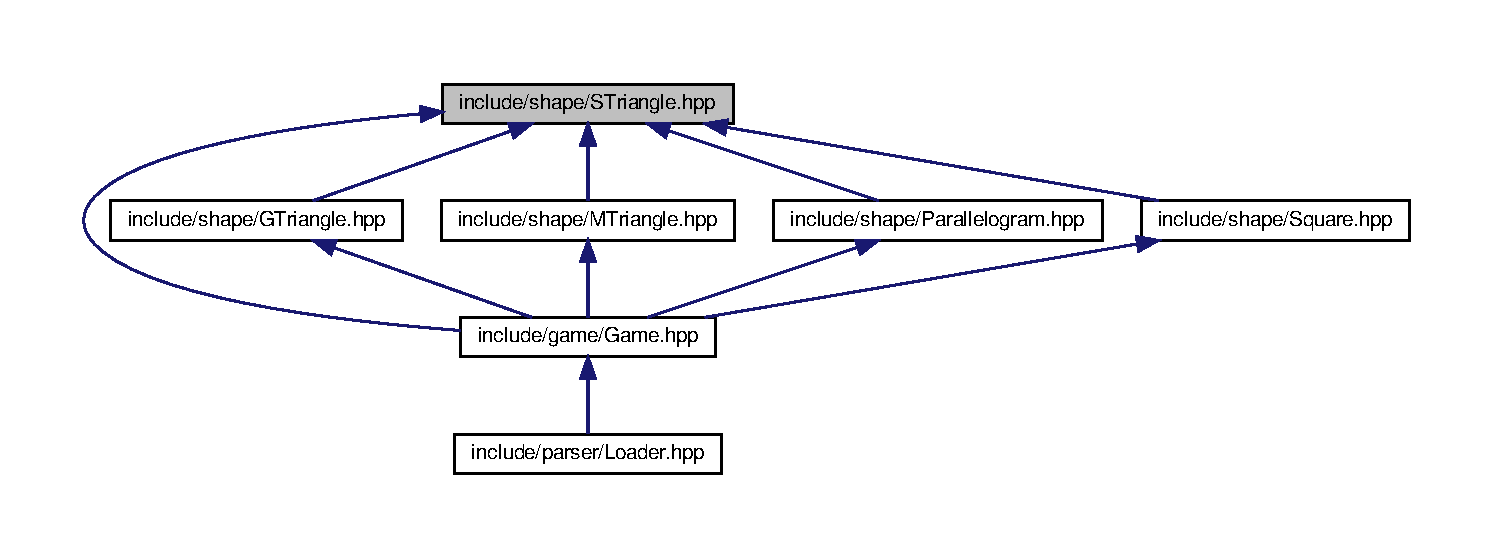
\includegraphics[width=350pt]{STriangle_8hpp__dep__incl}
\end{center}
\end{figure}
\subsection*{Classes}
\begin{DoxyCompactItemize}
\item 
class \hyperlink{classSTriangle}{S\+Triangle}
\begin{DoxyCompactList}\small\item\em Class of the small mTriangles. \end{DoxyCompactList}\end{DoxyCompactItemize}


\subsection{Detailed Description}
\hyperlink{classShape}{A_Shape} of Small Triangle.

\begin{DoxyAuthor}{Author}
Jérémie LE B\+A\+S\+T\+A\+RD 
\end{DoxyAuthor}
\begin{DoxyVersion}{Version}
1.\+0 
\end{DoxyVersion}

\hypertarget{Point_8hpp}{}\section{include/utils/\+Point.hpp File Reference}
\label{Point_8hpp}\index{include/utils/\+Point.\+hpp@{include/utils/\+Point.\+hpp}}


\hyperlink{classPoint}{Point} for every shape and menu.  


{\ttfamily \#include $<$functional$>$}\newline
Include dependency graph for Point.\+hpp\+:\nopagebreak
\begin{figure}[H]
\begin{center}
\leavevmode
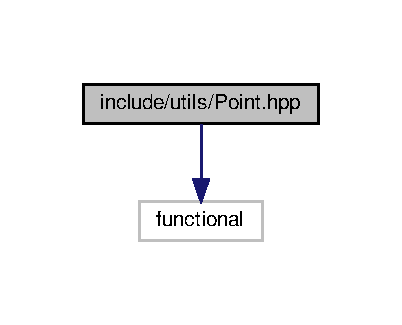
\includegraphics[width=193pt]{Point_8hpp__incl}
\end{center}
\end{figure}
This graph shows which files directly or indirectly include this file\+:
\nopagebreak
\begin{figure}[H]
\begin{center}
\leavevmode
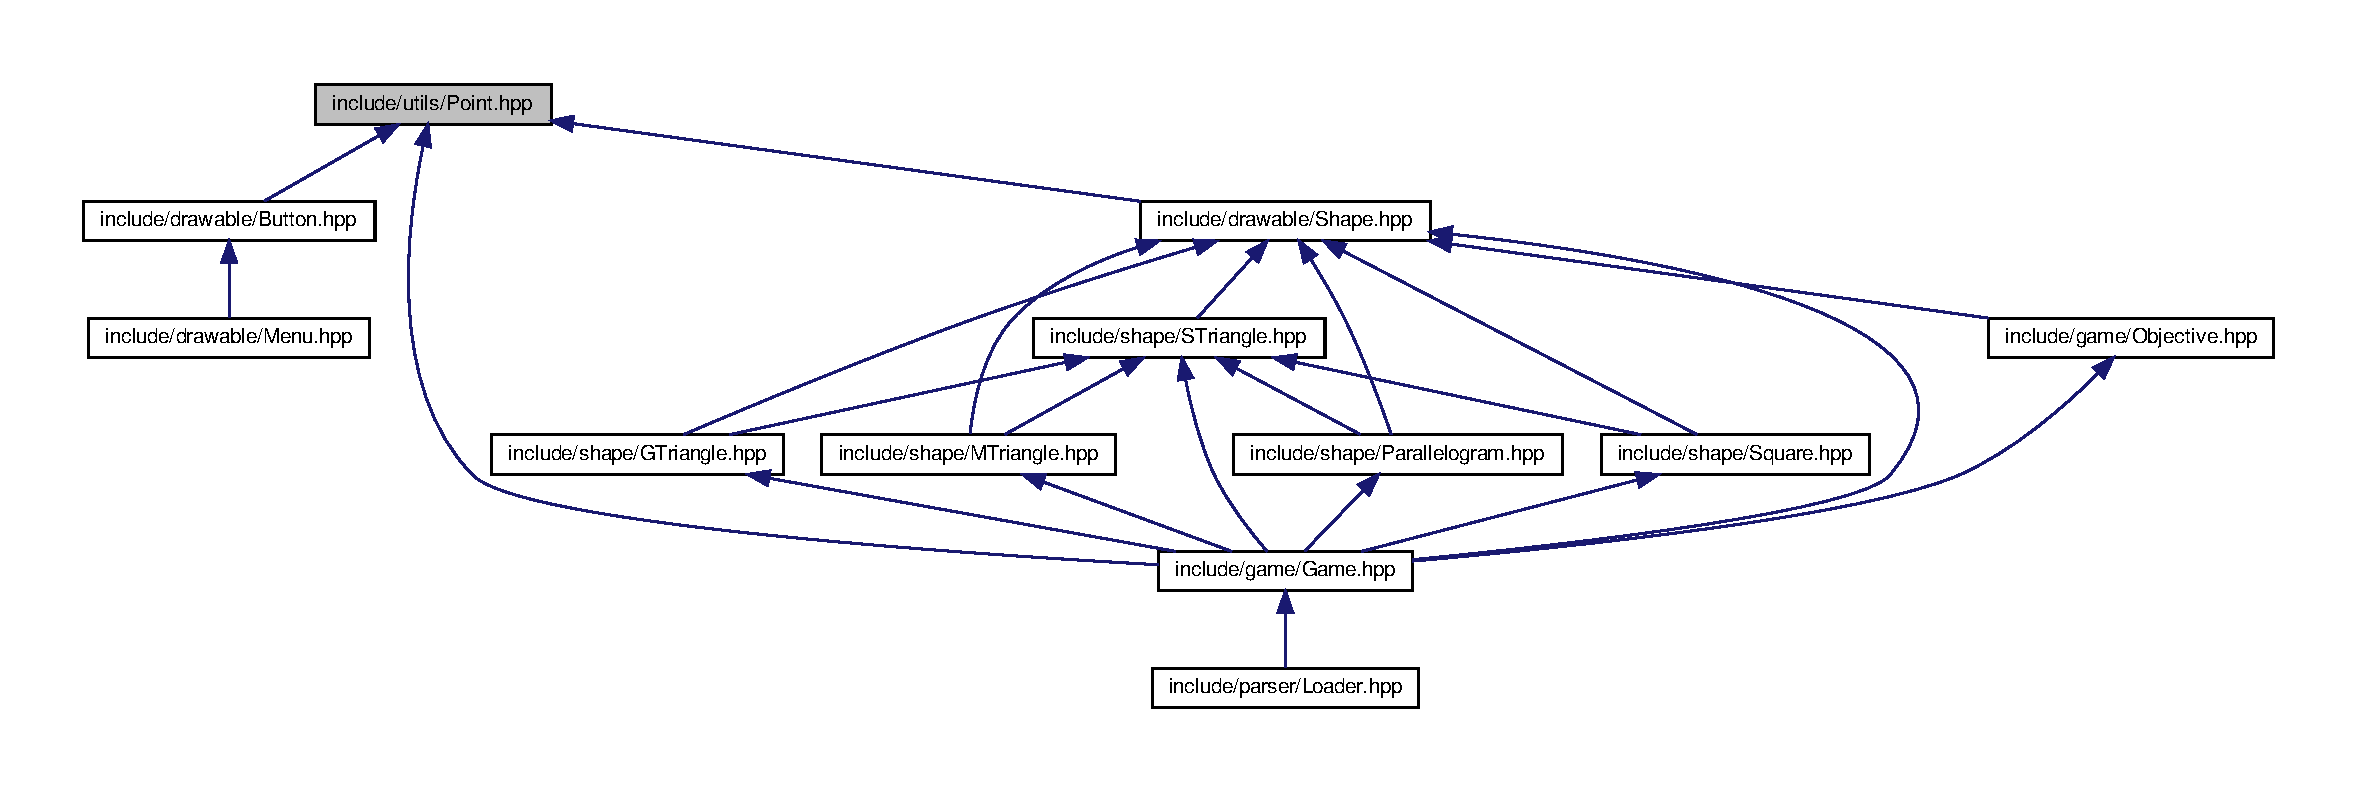
\includegraphics[width=350pt]{Point_8hpp__dep__incl}
\end{center}
\end{figure}
\subsection*{Classes}
\begin{DoxyCompactItemize}
\item 
class \hyperlink{classPoint}{Point$<$ T $>$}
\begin{DoxyCompactList}\small\item\em Class of a \hyperlink{classPoint}{Point}. \end{DoxyCompactList}\item 
struct \hyperlink{structPoint_1_1hash__point}{Point$<$ T $>$\+::hash\+\_\+point}
\end{DoxyCompactItemize}


\subsection{Detailed Description}
\hyperlink{classPoint}{Point} for every shape and menu. 

\begin{DoxyAuthor}{Author}
Jérémie LE B\+A\+S\+T\+A\+RD 
\end{DoxyAuthor}
\begin{DoxyVersion}{Version}
1.\+0 
\end{DoxyVersion}

%--- End generated contents ---

% Index
\backmatter
\newpage
\phantomsection
\clearemptydoublepage
\addcontentsline{toc}{chapter}{Index}
\printindex

\end{document}
